%-------------------------------------------------------------------------------
% PACKAGES AND OTHER DOCUMENT CONFIGURATIONS
%-------------------------------------------------------------------------------

\documentclass[11pt,fleqn]{book} % Default font size and left-justified equations

\usepackage[top=3cm,bottom=3cm,left=3.2cm,right=3.2cm,headsep=10pt,a4paper]{geometry} % Page margins

\usepackage{kotex}
\usepackage[unicode]{hyperref}

\usepackage{xcolor} % Required for specifying colors by name
\definecolor{ocre}{RGB}{243,102,25} % Define the orange color used for highlighting throughout the book

% Font Settings
\usepackage{avant} % Use the Avantgarde font for headings
%\usepackage{times} % Use the Times font for headings
\usepackage{mathptmx} % Use the Adobe Times Roman as the default text font together with math symbols from the Symbol, Chancery and Computer Modern fonts

\usepackage{microtype} % Slightly tweak font spacing for aesthetics
%\usepackage[utf8]{inputenc} % Required for including letters with accents
%\usepackage[T1]{fontenc} % Use 8-bit encoding that has 256 glyphs

% Bibliography
\usepackage[style=alphabetic,sorting=nyt,sortcites=true,autopunct=true,babel=hyphen,hyperref=true,abbreviate=false,backref=true,backend=biber]{biblatex}

\addbibresource{bibliography.bib} % BibTeX bibliography file
\defbibheading{bibempty}{}

% Index
\usepackage{calc} % For simpler calculation - used for spacing the index letter headings correctly
\usepackage{makeidx} % Required to make an index
\makeindex % Tells LaTeX to create the files required for indexing

\usepackage{tikz}
\newcommand*\circled[1]{\tikz[baseline=(char.base)]{
            \node[shape=circle,draw,inner sep=1pt] (char) {#1};}}
\newcounter{num}
% \newcounter{num}\setcounter{num}{0}
% \stepcounter{num}\circled{\thenum}
%-------------------------------------------------------------------------------

% -*- root: main.tex -*-
%----------------------------------------------------------------------------------------
%	VARIOUS REQUIRED PACKAGES
%----------------------------------------------------------------------------------------

\usepackage{titlesec} % Allows customization of titles

\usepackage{graphicx} % Required for including pictures
\graphicspath{{pictures/}} % Specifies the directory where pictures are stored

\usepackage{lipsum} % Inserts dummy text

\usepackage{tikz} % Required for drawing custom shapes

\usepackage[english]{babel} % English language/hyphenation

\usepackage{enumitem} % Customize lists
\setlist{nolistsep} % Reduce spacing between bullet points and numbered lists

\usepackage{booktabs} % Required for nicer horizontal rules in tables

\usepackage{eso-pic} % Required for specifying an image background in the title page

%----------------------------------------------------------------------------------------
%	MAIN TABLE OF CONTENTS
%----------------------------------------------------------------------------------------

\usepackage{titletoc} % Required for manipulating the table of contents

\contentsmargin{0cm} % Removes the default margin
% Chapter text styling
\titlecontents{chapter}[1.25cm] % Indentation
{\addvspace{15pt}\large\sffamily\bfseries} % Spacing and font options for chapters
{\color{ocre!60}\contentslabel[\Large\thecontentslabel]{1.25cm}\color{ocre}} % Chapter number
{}  
{\color{ocre!60}\normalsize\sffamily\bfseries\;\titlerule*[.5pc]{.}\;\thecontentspage} % Page number
% Section text styling
\titlecontents{section}[1.25cm] % Indentation
{\addvspace{5pt}\sffamily\bfseries} % Spacing and font options for sections
{\contentslabel[\thecontentslabel]{1.25cm}} % Section number
{}
{\sffamily\hfill\color{black}\thecontentspage} % Page number
[]
% Subsection text styling
\titlecontents{subsection}[1.25cm] % Indentation
{\addvspace{1pt}\sffamily\small} % Spacing and font options for subsections
{\contentslabel[\thecontentslabel]{1.25cm}} % Subsection number
{}
{\sffamily\;\titlerule*[.5pc]{.}\;\thecontentspage} % Page number
[] 

%----------------------------------------------------------------------------------------
%	MINI TABLE OF CONTENTS IN CHAPTER HEADS
%----------------------------------------------------------------------------------------

% Section text styling
\titlecontents{lsection}[0em] % Indendating
{\footnotesize\sffamily} % Font settings
{}
{}
{}

% Subsection text styling
\titlecontents{lsubsection}[.5em] % Indentation
{\normalfont\footnotesize\sffamily} % Font settings
{}
{}
{}
 
%----------------------------------------------------------------------------------------
%	PAGE HEADERS
%----------------------------------------------------------------------------------------

\usepackage{fancyhdr} % Required for header and footer configuration

\pagestyle{fancy}
\renewcommand{\chaptermark}[1]{\markboth{\sffamily\normalsize\bfseries\chaptername\ \thechapter.\ #1}{}} % Chapter text font settings
\renewcommand{\sectionmark}[1]{\markright{\sffamily\normalsize\thesection\hspace{5pt}#1}{}} % Section text font settings
\fancyhf{} \fancyhead[LE,RO]{\sffamily\normalsize\thepage} % Font setting for the page number in the header
\fancyhead[LO]{\rightmark} % Print the nearest section name on the left side of odd pages
\fancyhead[RE]{\leftmark} % Print the current chapter name on the right side of even pages
\renewcommand{\headrulewidth}{0.5pt} % Width of the rule under the header
\addtolength{\headheight}{2.5pt} % Increase the spacing around the header slightly
\renewcommand{\footrulewidth}{0pt} % Removes the rule in the footer
\fancypagestyle{plain}{\fancyhead{}\renewcommand{\headrulewidth}{0pt}} % Style for when a plain pagestyle is specified

% Removes the header from odd empty pages at the end of chapters
\makeatletter
\renewcommand{\cleardoublepage}{
\clearpage\ifodd\c@page\else
\hbox{}
\vspace*{\fill}
\thispagestyle{empty}
\newpage
\fi}

%----------------------------------------------------------------------------------------
%	THEOREM STYLES
%----------------------------------------------------------------------------------------

\usepackage{amsmath,amsfonts,amssymb,amsthm} % For math equations, theorems, symbols, etc

\newcommand{\intoo}[2]{\mathopen{]}#1\,;#2\mathclose{[}}
\newcommand{\ud}{\mathop{\mathrm{{}d}}\mathopen{}}
\newcommand{\intff}[2]{\mathopen{[}#1\,;#2\mathclose{]}}
\newtheorem{notation}{Notation}[chapter]

%%%%%%%%%%%%%%%%%%%%%%%%%%%%%%%%%%%%%%%%%%%%%%%%%%%%%%%%%%%%%%%%%%%%%%%%%%%
%%%%%%%%%%%%%%%%%%%% dedicated to boxed/framed environements %%%%%%%%%%%%%%
%%%%%%%%%%%%%%%%%%%%%%%%%%%%%%%%%%%%%%%%%%%%%%%%%%%%%%%%%%%%%%%%%%%%%%%%%%%
\newtheoremstyle{ocrenumbox}% % Theorem style name
{0pt}% Space above
{0pt}% Space below
{\normalfont}% % Body font
{}% Indent amount
{\small\bf\sffamily\color{ocre}}% % Theorem head font
{\;}% Punctuation after theorem head
{0.25em}% Space after theorem head
{\small\sffamily\color{ocre}\thmname{#1}\nobreakspace\thmnumber{\@ifnotempty{#1}{}\@upn{#2}}% Theorem text (e.g. Theorem 2.1)
\thmnote{\nobreakspace\the\thm@notefont\sffamily\bfseries\color{black}---\nobreakspace#3.}} % Optional theorem note
\renewcommand{\qedsymbol}{$\blacksquare$}% Optional qed square

\newtheoremstyle{blacknumex}% Theorem style name
{5pt}% Space above
{5pt}% Space below
{\normalfont}% Body font
{} % Indent amount
{\small\bf\sffamily}% Theorem head font
{\;}% Punctuation after theorem head
{0.25em}% Space after theorem head
{\small\sffamily{\tiny\ensuremath{\blacksquare}}\nobreakspace\thmname{#1}\nobreakspace\thmnumber{\@ifnotempty{#1}{}\@upn{#2}}% Theorem text (e.g. Theorem 2.1)
\thmnote{\nobreakspace\the\thm@notefont\sffamily\bfseries---\nobreakspace#3.}}% Optional theorem note

\newtheoremstyle{blacknumbox} % Theorem style name
{0pt}% Space above
{0pt}% Space below
{\normalfont}% Body font
{}% Indent amount
{\small\bf\sffamily}% Theorem head font
{\;}% Punctuation after theorem head
{0.25em}% Space after theorem head
{\small\sffamily\thmname{#1}\nobreakspace\thmnumber{\@ifnotempty{#1}{}\@upn{#2}}% Theorem text (e.g. Theorem 2.1)
\thmnote{\nobreakspace\the\thm@notefont\sffamily\bfseries---\nobreakspace#3.}}% Optional theorem note

%%%%%%%%%%%%%%%%%%%%%%%%%%%%%%%%%%%%%%%%%%%%%%%%%%%%%%%%%%%%%%%%%%%%%%%%%%%
%%%%%%%%%%%%% dedicated to non-boxed/non-framed environements %%%%%%%%%%%%%
%%%%%%%%%%%%%%%%%%%%%%%%%%%%%%%%%%%%%%%%%%%%%%%%%%%%%%%%%%%%%%%%%%%%%%%%%%%
\newtheoremstyle{ocrenum}% % Theorem style name
{5pt}% Space above
{5pt}% Space below
{\normalfont}% % Body font
{}% Indent amount
{\small\bf\sffamily\color{ocre}}% % Theorem head font
{\;}% Punctuation after theorem head
{0.25em}% Space after theorem head
{\small\sffamily\color{ocre}\thmname{#1}\nobreakspace\thmnumber{\@ifnotempty{#1}{}\@upn{#2}}% Theorem text (e.g. Theorem 2.1)
\thmnote{\nobreakspace\the\thm@notefont\sffamily\bfseries\color{black}---\nobreakspace#3.}} % Optional theorem note
\renewcommand{\qedsymbol}{$\blacksquare$}% Optional qed square
\makeatother

% Defines the theorem text style for each type of theorem to one of the three styles above
\newcounter{dummy} 
\numberwithin{dummy}{section}
\theoremstyle{ocrenumbox}
\newtheorem{theoremeT}[dummy]{Theorem}
\newtheorem{problem}{Problem}[chapter]
% \newtheorem{exerciseT}{Exercise}[chapter]
\newtheorem{exerciseT}{참고}
\theoremstyle{blacknumex}
\newtheorem{exampleT}{Example}[chapter]
\theoremstyle{blacknumbox}
% \newtheorem{vocabulary}{Vocabulary}[chapter]
% \newtheorem{definitionT}{Definition}[section]
\newtheorem{vocabulary}{ROS용어}
\newtheorem{definitionT}{ROS용어}
\newtheorem*{definitionT*}{ROS용어}
\newtheorem{corollaryT}[dummy]{Corollary}
\theoremstyle{ocrenum}
\newtheorem{proposition}[dummy]{Proposition}

%----------------------------------------------------------------------------------------
%	DEFINITION OF COLORED BOXES
%----------------------------------------------------------------------------------------

\RequirePackage[framemethod=default]{mdframed} % Required for creating the theorem, definition, exercise and corollary boxes

% Theorem box
\newmdenv[skipabove=7pt,
skipbelow=7pt,
backgroundcolor=black!5,
linecolor=ocre,
innerleftmargin=5pt,
innerrightmargin=5pt,
innertopmargin=5pt,
leftmargin=0cm,
rightmargin=0cm,
innerbottommargin=5pt]{tBox}

% Exercise box	  
\newmdenv[skipabove=7pt,
skipbelow=7pt,
rightline=false,
leftline=true,
topline=false,
bottomline=false,
backgroundcolor=ocre!10,
linecolor=ocre,
innerleftmargin=5pt,
innerrightmargin=5pt,
innertopmargin=5pt,
innerbottommargin=5pt,
leftmargin=0cm,
rightmargin=0cm,
linewidth=4pt]{eBox}	

% Definition box
\newmdenv[skipabove=7pt,
skipbelow=7pt,
rightline=false,
leftline=true,
topline=false,
bottomline=false,
linecolor=ocre,
innerleftmargin=5pt,
innerrightmargin=5pt,
innertopmargin=0pt,
leftmargin=0cm,
rightmargin=0cm,
linewidth=4pt,
innerbottommargin=0pt]{dBox}	

% Corollary box
\newmdenv[skipabove=7pt,
skipbelow=7pt,
rightline=false,
leftline=true,
topline=false,
bottomline=false,
linecolor=gray,
backgroundcolor=black!5,
innerleftmargin=5pt,
innerrightmargin=5pt,
innertopmargin=5pt,
leftmargin=0cm,
rightmargin=0cm,
linewidth=4pt,
innerbottommargin=5pt]{cBox}

% Creates an environment for each type of theorem and assigns it a theorem text style from the "Theorem Styles" section above and a colored box from above
\newenvironment{theorem}{\begin{tBox}\begin{theoremeT}}{\end{theoremeT}\end{tBox}}
\newenvironment{exercise}{\begin{eBox}\begin{exerciseT}}{\hfill{\color{ocre}\tiny\ensuremath{\blacksquare}}\end{exerciseT}\end{eBox}}
\newenvironment{definition}{\begin{dBox}\begin{definitionT}}{\end{definitionT}\end{dBox}}
\newenvironment{definition*}{\begin{dBox}\begin{definitionT*}}{\end{definitionT*}\end{dBox}}
\newenvironment{example}{\begin{exampleT}}{\hfill{\tiny\ensuremath{\blacksquare}}\end{exampleT}}		
\newenvironment{corollary}{\begin{cBox}\begin{corollaryT}}{\end{corollaryT}\end{cBox}}	

%----------------------------------------------------------------------------------------
%	REMARK ENVIRONMENT
%----------------------------------------------------------------------------------------

\newenvironment{remark}{\par\vspace{10pt}\small % Vertical white space above the remark and smaller font size
\begin{list}{}{
\leftmargin=35pt % Indentation on the left
\rightmargin=25pt}\item\ignorespaces % Indentation on the right
\makebox[-2.5pt]{\begin{tikzpicture}[overlay]
\node[draw=ocre!60,line width=1pt,circle,fill=ocre!25,font=\sffamily\bfseries,inner sep=2pt,outer sep=0pt] at (-15pt,0pt){\textcolor{ocre}{R}};\end{tikzpicture}} % Orange R in a circle
\advance\baselineskip -1pt}{\end{list}\vskip5pt} % Tighter line spacing and white space after remark

%----------------------------------------------------------------------------------------
%	SECTION NUMBERING IN THE MARGIN
%----------------------------------------------------------------------------------------

\makeatletter
\renewcommand{\@seccntformat}[1]{\llap{\textcolor{ocre}{\csname the#1\endcsname}\hspace{1em}}}                    
\renewcommand{\section}{\@startsection{section}{1}{\z@}
{-4ex \@plus -1ex \@minus -.4ex}
{1ex \@plus.2ex }
{\normalfont\large\sffamily\bfseries}}
\renewcommand{\subsection}{\@startsection {subsection}{2}{\z@}
{-3ex \@plus -0.1ex \@minus -.4ex}
{0.5ex \@plus.2ex }
{\normalfont\sffamily\bfseries}}
\renewcommand{\subsubsection}{\@startsection {subsubsection}{3}{\z@}
{-2ex \@plus -0.1ex \@minus -.2ex}
{.2ex \@plus.2ex }
{\normalfont\small\sffamily\bfseries}}                        
\renewcommand\paragraph{\@startsection{paragraph}{4}{\z@}
{-2ex \@plus-.2ex \@minus .2ex}
{.1ex}
{\normalfont\small\sffamily\bfseries}}

%----------------------------------------------------------------------------------------
%	HYPERLINKS IN THE DOCUMENTS
%----------------------------------------------------------------------------------------

% For an unclear reason, the package should be loaded now and not later
\usepackage{hyperref}
\hypersetup{hidelinks,backref=true,pagebackref=true,hyperindex=true,colorlinks=false,breaklinks=true,urlcolor= ocre,bookmarks=true,bookmarksopen=false,pdftitle={Title},pdfauthor={Author}}

%----------------------------------------------------------------------------------------
%	CHAPTER HEADINGS
%----------------------------------------------------------------------------------------

% The set-up below should be (sadly) manually adapted to the overall margin page septup controlled by the geometry package loaded in the main.tex document. It is possible to implement below the dimensions used in the goemetry package (top,bottom,left,right)... TO BE DONE

\newcommand{\thechapterimage}{}
\newcommand{\chapterimage}[1]{\renewcommand{\thechapterimage}{#1}}

% Numbered chapters with mini tableofcontents
\def\thechapter{\arabic{chapter}}
\def\@makechapterhead#1{
\thispagestyle{empty}
{\centering \normalfont\sffamily
\ifnum \c@secnumdepth >\m@ne
\if@mainmatter
\startcontents
\begin{tikzpicture}[remember picture,overlay]
\node at (current page.north west)
{\begin{tikzpicture}[remember picture,overlay]
\node[anchor=north west,inner sep=0pt] at (0,0) {\includegraphics[width=\paperwidth]{\thechapterimage}};
%%%%%%%%%%%%%%%%%%%%%%%%%%%%%%%%%%%%%%%%%%%%%%%%%%%%%%%%%%%%%%%%%%%%%%%%%%%%%%%%%%%%%
% Commenting the 3 lines below removes the small contents box in the chapter heading
% \fill[color=ocre!10!white,opacity=.6] (1cm,0) rectangle (8cm,-7cm);
% \node[anchor=north west] at (1.1cm,.35cm) {\parbox[t][8cm][t]{6.5cm}{\huge\bfseries\flushleft \printcontents{l}{1}{\setcounter{tocdepth}{2}}}};
\draw[anchor=west] (5cm,-9cm) node [rounded corners=20pt,fill=ocre!10!white,text opacity=1,draw=ocre,draw opacity=1,line width=1.5pt,fill opacity=.6,inner sep=12pt]{\huge\sffamily\bfseries\textcolor{black}{\thechapter. #1\strut\makebox[22cm]{}}};
%%%%%%%%%%%%%%%%%%%%%%%%%%%%%%%%%%%%%%%%%%%%%%%%%%%%%%%%%%%%%%%%%%%%%%%%%%%%%%%%%%%%%
\end{tikzpicture}};
\end{tikzpicture}}
\par\vspace*{230\p@}
\fi
\fi}

% Unnumbered chapters without mini tableofcontents (could be added though) 
\def\@makeschapterhead#1{
\thispagestyle{empty}
{\centering \normalfont\sffamily
\ifnum \c@secnumdepth >\m@ne
\if@mainmatter
\begin{tikzpicture}[remember picture,overlay]
\node at (current page.north west)
{\begin{tikzpicture}[remember picture,overlay]
\node[anchor=north west,inner sep=0pt] at (0,0) {\includegraphics[width=\paperwidth]{\thechapterimage}};
\draw[anchor=west] (5cm,-9cm) node [rounded corners=20pt,fill=ocre!10!white,fill opacity=.6,inner sep=12pt,text opacity=1,draw=ocre,draw opacity=1,line width=1.5pt]{\huge\sffamily\bfseries\textcolor{black}{#1\strut\makebox[22cm]{}}};
\end{tikzpicture}};
\end{tikzpicture}}
\par\vspace*{230\p@}
\fi
\fi
}
\makeatother % Insert the commands.tex file which contains the majority of the structure behind the template
% -*- root: main.tex -*-
% https://www.sharelatex.com/learn/Code_listing

\usepackage{listings}
\usepackage{color}

\renewcommand\lstlistingname{Code}

\definecolor{codegreen}{rgb}{0,0.6,0}
\definecolor{codegray}{rgb}{0.5,0.5,0.5}
\definecolor{codemauve}{rgb}{0.58,0,0.82}
\definecolor{backcolour}{rgb}{0.95,0.95,0.92}

\newcommand*{\Comment}[1]{\hfill\makebox[3.0cm][l]{#1}}

\lstdefinelanguage{ROS}{
  keywords={roscd,rospd,rosd,rosls,rosed,roscp,roscore,rosrun,roslaunch,rosclean,rostopic,rosservice,rosnode,rosparam,rosmsg,rossrv,roswtf,rosversion,rosbag,catkin_create_pkg,catkin_eclipse,catkin_find,catkin_generate_changelog,catkin_init_workspace,catkin_make,rqt},
  comment=[l]{//},
  literate={\$}{{\textcolor{red}\$}}1   
}

\lstset{
  xleftmargin=5pt,
  xrightmargin=5pt,
  backgroundcolor=\color{backcolour},   % choose the background color; you must add \usepackage{color} or \usepackage{xcolor}
  basicstyle=\footnotesize,        % the size of the fonts that are used for the code
  breakatwhitespace=false,         % sets if automatic breaks should only happen at whitespace
  breaklines=true,                 % sets automatic line breaking
  captionpos=b,                    % sets the caption-position to bottom
  commentstyle=\color{codegreen},    % comment style
  deletekeywords={...},            % if you want to delete keywords from the given language
  escapeinside={\%*}{*)},          % if you want to add LaTeX within your code
  extendedchars=true,              % lets you use non-ASCII characters; for 8-bits encodings only, does not work with UTF-8
  frame=single,                    % adds a frame around the code
  keepspaces=true,                 % keeps spaces in text, useful for keeping indentation of code (possibly needs columns=flexible)
  keywordstyle=\color{blue},       % keyword style
  language=C++,                    % the language of the code
  morekeywords={*,...},            % if you want to add more keywords to the set
  numbers=none,                    % where to put the line-numbers; possible values are (none, left, right)
  numbersep=5pt,                   % how far the line-numbers are from the code
  numberstyle=\tiny\color{codegray}, % the style that is used for the line-numbers
  rulecolor=\color{black},         % if not set, the frame-color may be changed on line-breaks within not-black text (e.g. comments (green here))
  showspaces=false,                % show spaces everywhere adding particular underscores; it overrides 'showstringspaces'
  showstringspaces=false,          % underline spaces within strings only
  showtabs=false,                  % show tabs within strings adding particular underscores
  stepnumber=1,                    % the step between two line-numbers. If it's 1, each line will be numbered
  stringstyle=\color{codemauve},     % string literal style
  tabsize=2,                       % sets default tabsize to 2 spaces
  title=\lstname                   % show the filename of files included with \lstinputlisting; also try caption instead of title
  % morecomment=[l]{//}              % displays comments in italics (language dependent)
} % parameters to insert source code

\begin{document}

%-------------------------------------------------------------------------------
% TITLE PAGE
%-------------------------------------------------------------------------------

\begingroup
\thispagestyle{empty}
\AddToShipoutPicture*{\put(6,5){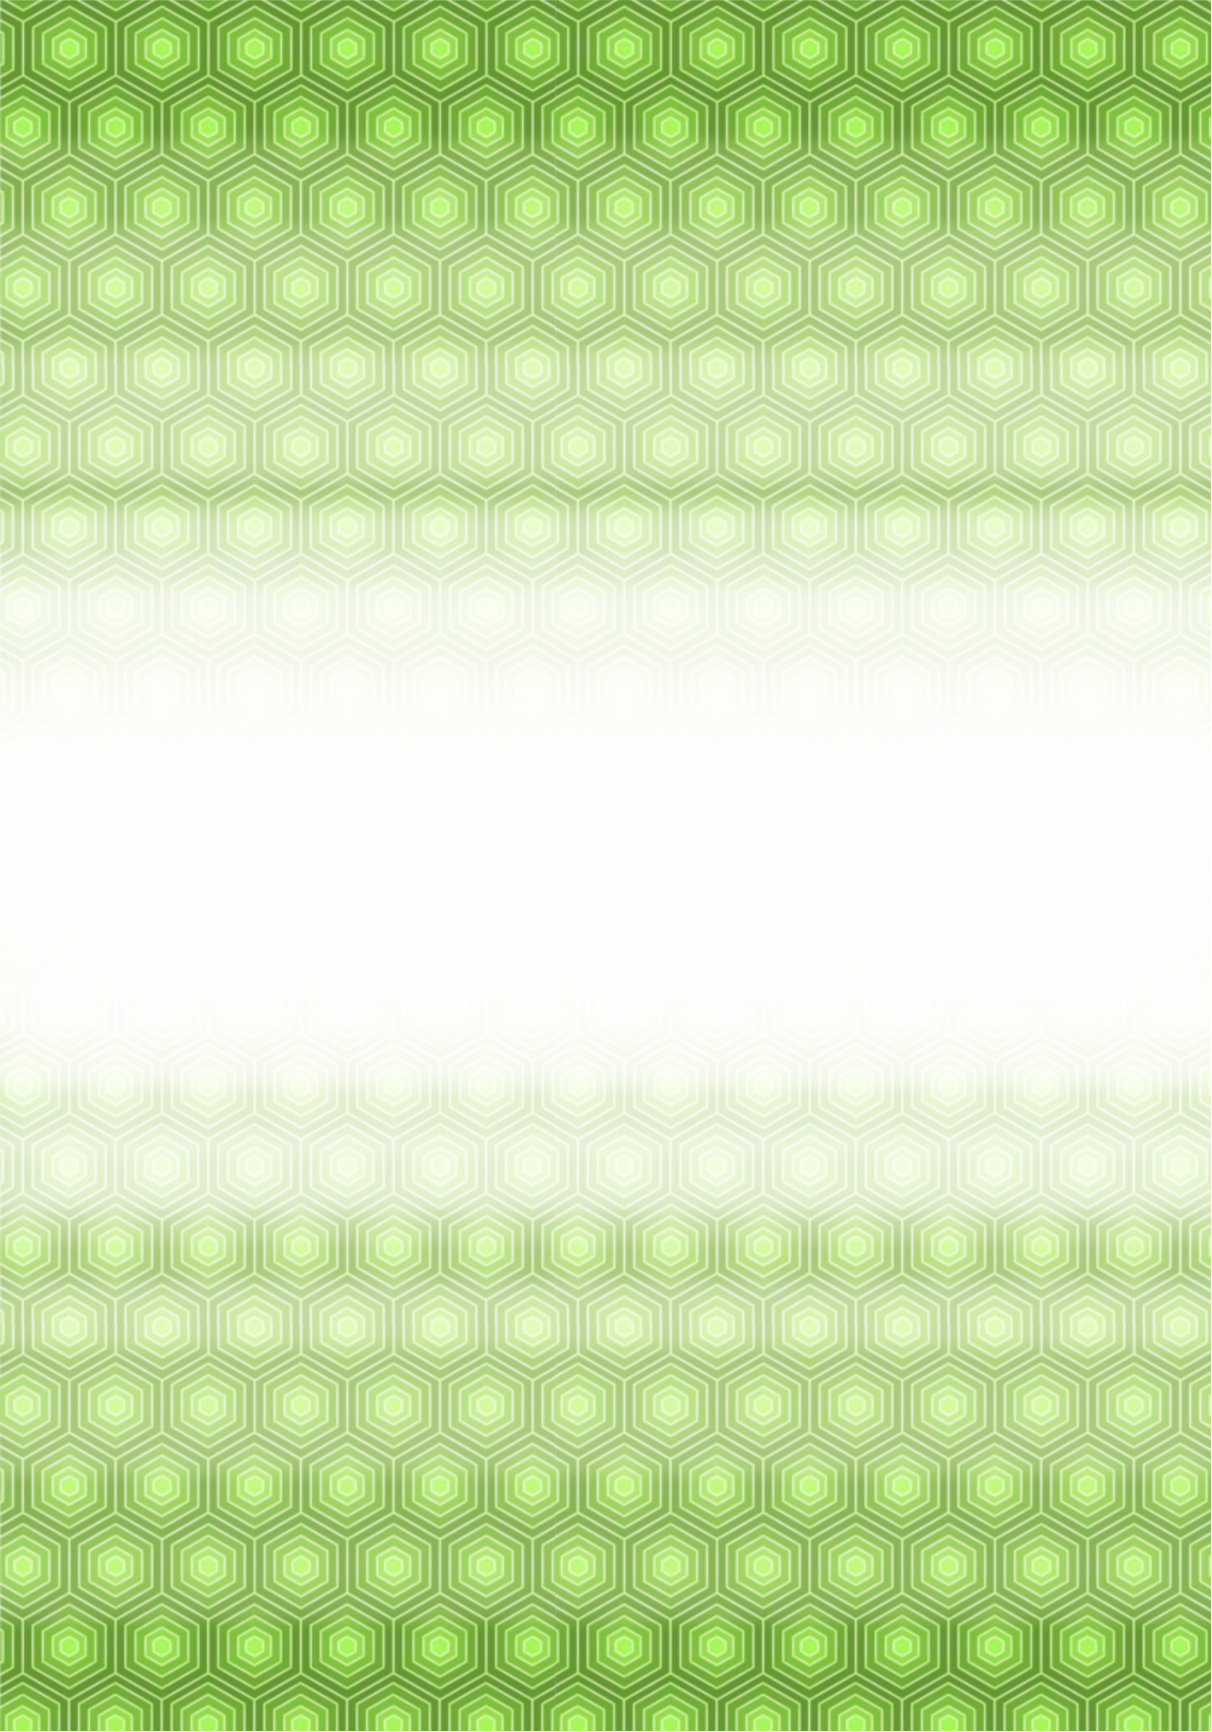
\includegraphics[scale=1]{cover}}} % Image background
\centering
\vspace*{3cm}
\begin{figure}[h]
\centering\hspace{30pt}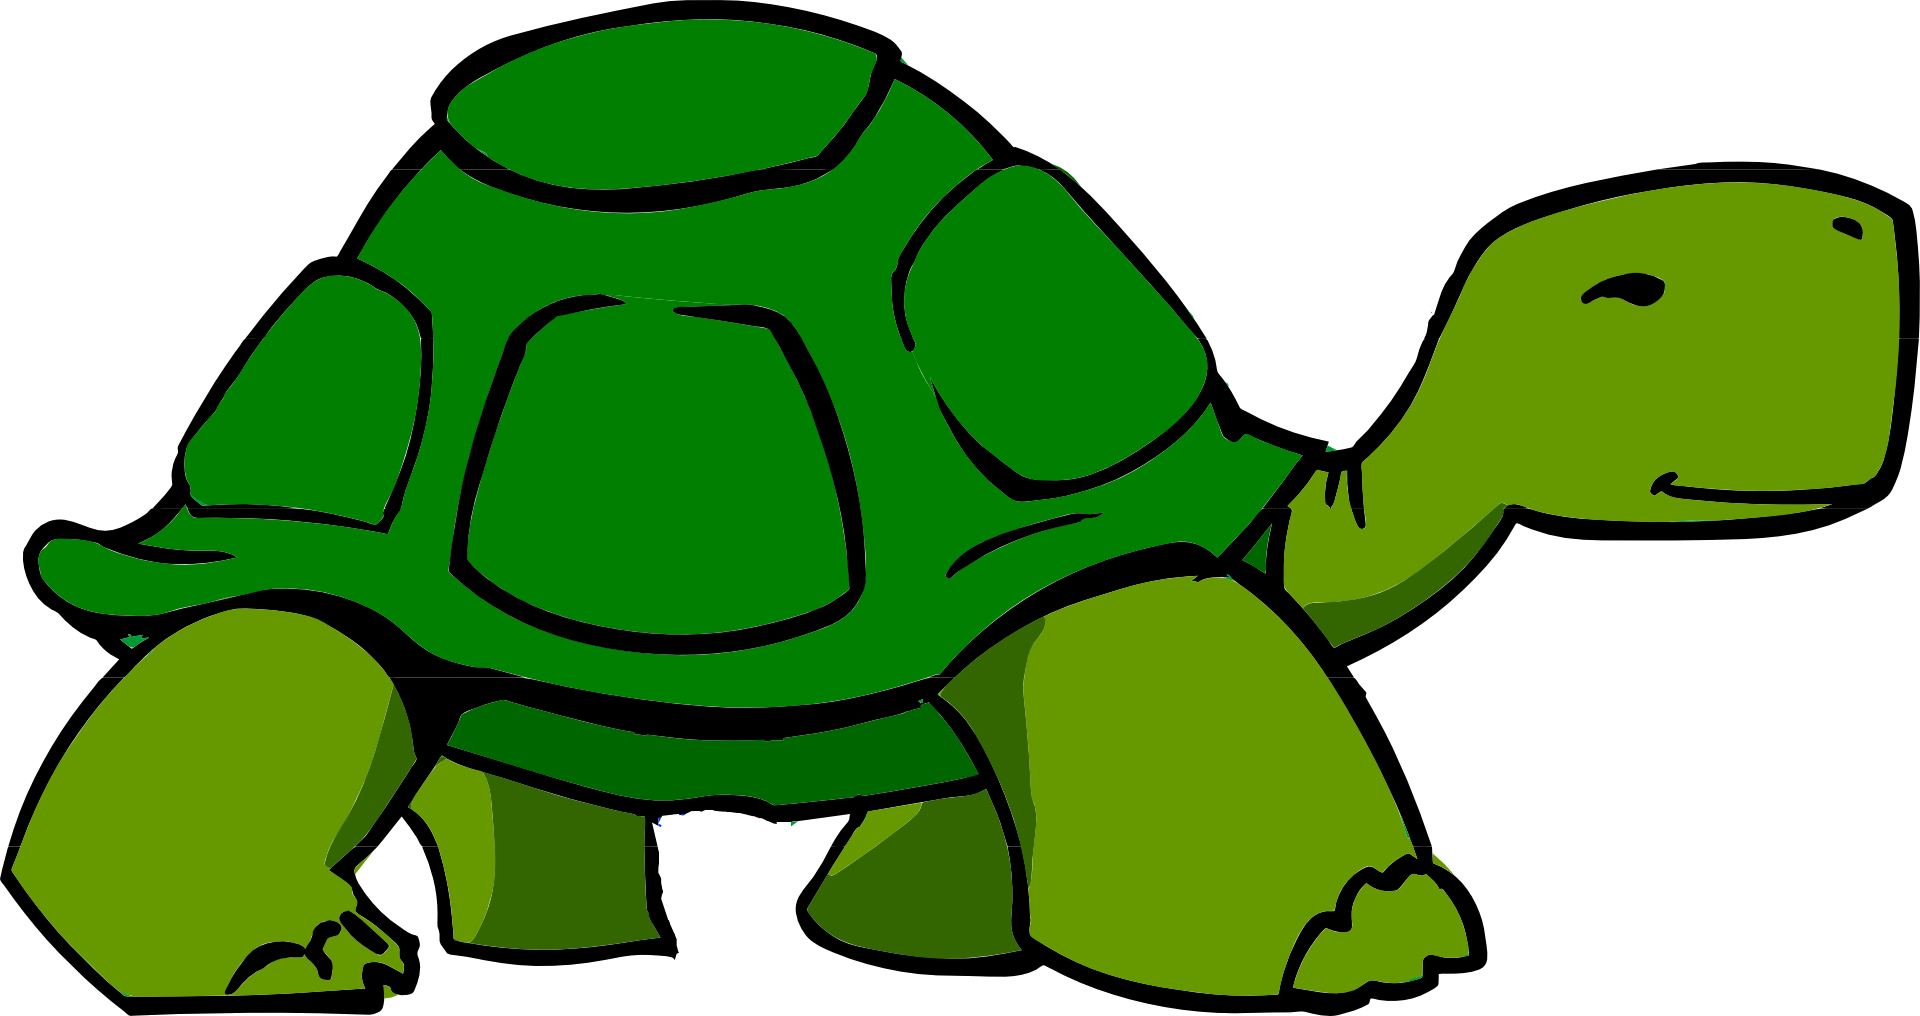
\includegraphics[scale=0.05]{turtle}
\end{figure}
\vspace*{1cm}
\par\normalfont\fontsize{50}{50}\sffamily\selectfont
로봇 프로그래밍\\
\textcolor{magenta}{\textbf{ROS}}로 시작하자!\par % Book title
{\Huge -로봇 운영 체제-}\\ % Sub book title
{\Huge \textit{(Robot Operating System)}}\par
\vspace*{6cm}
{\large 표윤석 지음}\par
{\large WWW.OROCA.ORG}\par
\endgroup

%-------------------------------------------------------------------------------
% COPYRIGHT PAGE
%-------------------------------------------------------------------------------

\newpage
~\vfill
\thispagestyle{empty}

\noindent Copyright \copyright\ 2014 Yoonseok Pyo\\ % Copyright notice

\noindent \textsc{Published by Publisher}\\ % Publisher

\noindent \textsc{oroca.org}\\ % URL

\noindent Licensed under the Creative Commons Attribution-NonCommercial 4.0 Unported License (the ``License''). You may not use this file except in compliance with the License. You may obtain a copy of the License at \url{http://creativecommons.org/licenses/by-nc/4.0}. Unless required by applicable law or agreed to in writing, software distributed under the License is distributed on an \textsc{``as is'' basis, without warranties or conditions of any kind}, either express or implied. See the License for the specific language governing permissions and limitations under the License.\\ % License information

\noindent \textit{First printing, December 2014} % Printing/edition date

%-------------------------------------------------------------------------------
% TABLE OF CONTENTS
%-------------------------------------------------------------------------------

\chapterimage{chapter_head_14.pdf} % Table of contents heading image

\pagestyle{empty} % No headers

\tableofcontents % Print the table of contents itself

\cleardoublepage % Forces the first chapter to start on an odd page so it's on the right

\pagestyle{fancy} % Print headers again

%-------------------------------------------------------------------------------
% CHAPTER  LIST
%-------------------------------------------------------------------------------

\setlength\parindent{1em}
%-------------------------------------------------------------------------------
\chapterimage{chapter_head_2.pdf} % Chapter heading image

%-------------------------------------------------------------------------------
\chapter{로봇 운영 체제}

%-------------------------------------------------------------------------------
\section{로봇 소프트웨어 플랫폼}\index{로봇 소프트웨어 플랫폼}

%-------------------------------------------------------------------------------
\subsection{플랫폼이 가져온 변화}\index{플랫폼이 가져온 변화}

잠깐, 로봇 이야기가 아닌, 핸드폰에 대해서 이야기해보자. 불가 20년전만 하더라도 스마트폰과 같은 핸드폰이 지금과 같이 많은 사람들의 필수품이 되리라고는 생각지도 못했었다.
더욱이, 초기의 핸드폰은 핸드폰이라는 이름이 무상할 정도로 크고 무거운 무전기와 같았고, 가격은 상상을 초월할 정도로 비쌌으며, 성능은 떨어졌다.
이에 비하여 현재의 스마트폰은 가격도 저렴하고, 가볍고, 작고 사용하기도 편리하다는 것을 본다면 그 변화는 놀랍기까지 하다.

올해 2013년, 40주년이 된 세계 최초의 상용 핸드폰인 모토롤라 다이나택 8000의 경우\footnote{http://www.segye.com/content/html/2013/04/04/20130404004829.html}\footnote{CarToyBlog, "Happy 40th Birthday to the Cell Phone!",  http://blog.cartoys.com/date/2013/04/},\footnote{http://venma.tistory.com/entry/Motorola-DynaTAC-8000X}, 그 당시 가격으로 500만원대, 0.8Kg의 무게, 최대 통화시간 30분, 충전 10시간 소요, 최대 30개 전화번호 입력 정도만이 가능하였다.
그 뒤로 핸드폰 시장은 급성장하게 되었고, 현재의 스마트폰까지 이르렀다. 그리고, 지금은 우리에게는 없어서는 안되는 생활 필수 아이템이 되었다.

그렇다면 이러한 것이 가능했던 이유는 무엇이였을까? 

초기에 많은 핸드폰 관련 회사들은 기술 경쟁을 거듭하며, 슬림하면서도 가볍고 고화질, 고음질, 휴대성 등 자신들만의 특징들을 네세우며 새로운 기기들을 내놓았다.
그 당시만해도 핸드폰은 모델마다 하드웨어에 맞게 기능을 추가하기 위하여 하드웨어 의존적인 펌웨어 개발을 했다.
한 회사에만 수 십가지 기종이 있었을테고, 전세계적으로는 어땠을까?
상상할 수도 없는 규모이다.
목적은 다 비슷한데 통합되지 못하고 그렇게 개발자들은 죽어라~ 새로운 하드웨어 개발 일정에 맞추어 펌웨어 개발을 했고 이는 반복되었다.
새로운 하드웨어마다 의존적으로 개발하였기에 그 발전 속도는 떨어졌고, 의존성으로 인하여 관리 비용은 높기만 했다.
그리고 그 비용은 우리 소비자의 몫이였다. 

지금은 어떠한가?
안드로이드, iOS, 윈도우즈 등 대표적인 OS를 기반으로 개발자들이 힘을 모으게 되었고 이러한 소프트웨어 플랫폼을 기반으로 핸드폰이라는 하드웨어 플랫폼을 잘 몰라도 관련 어플리케이션 개발에 문제가 없게 되었다.
그리고, 앱 개발자라는 새로운 소프트웨어 직종을 생길 정도로 스마트폰 운영체제를 기반으로 한 개발 환경이 확립되었으며, 스마트폰 운영체제 관리팀 이외에도 스마트폰 회사, 앱 개발자, 심지어 일반 사용자들까지도 하나로 뭉쳐서 하드웨어와 소프트웨어를 통합하는 플랫폼은 진화의 진화를 거듭하게 되었다.
이는 핸드폰 뿐만아니라 개인컴퓨터 개발과 더불어 불어닥친 유닉스, 리눅스, 윈도우, OS X 등의 컴퓨터용 OS 도 마찬가지 양상이라고 볼 수 있다.

이러한 이유로는 하드웨어의 급성장과 필연적인 사용자들의 수요도 있었겠지만,  소프트웨어 플랫폼 기반으로 지식이 한데 모아져서 나온 결과라고 볼 수 있다.
이러한 소프트웨어 플랫폼은 하드웨어 플랫폼의 인터페이스를 통합시키게 만들고, 나아가 하드웨어를 몰라도 상위 단의 프로그램인 응용 프로그램에 집중할 수 있게 되었기 때문에 사용자들의 수요에 맞는 응용 제품이 나올 수 있었다고 생각된다. 

%-------------------------------------------------------------------------------
\subsection{플랫폼이 가져온 변화}\index{플랫폼이 가져온 변화}

최근, 로봇계도 마찬가지의 움직임을 보이고 있다. 스마트폰 OS 나 개인컴퓨터 OS 에 비하여 그 규모는 작고, 아직 발전 단계이기는 하지만 로봇 소프트웨어 플랫폼은 춘추전국시대라고 볼 수 있을 정도로 매우 활발하게 진행되고 있다.
아래의 리스트는 그 중에서 돋보이는 활동을 보이고 있는 그룹들의 로봇 소프트웨어 플랫폼이다.

\begin{itemize}
\item ERSP,Evolution robotics (회사)\footnote{http://www.evolution.com/products/ersp/}
\item MSRDS,Microsoft (회사)\footnote{http://msdn.microsoft.com/en-us/robotics/default.aspx}
\item OpenRTM,일본의 AIST (국립 연구소)\footnote{http://www.openrtm.org}
\item ROS,Open Source Robotics Foundation\footnote{http://www.osrfoundation.org/}
\item OROCOS,유럽\footnote{http://www.orocos.org/}
\item OPRoS,한국\footnote{http://www.opros.or.kr/}
\end{itemize}

위와 같이 많은 플랫폼들이 등장하고 있고, 현재도 다양한 접근방식으로 증가 추세에 있다.
너도나도 로봇계의 로봇 소프트웨에 플랫폼의 선두에 서고 싶기 때문일 것이다.
현재, 다양한 로봇 소프트웨어 플랫폼이 나오고 있지만, 어느 것이 좋다라고는 섣불리 말하기 어려운게 사실이다.
그러나, 언젠가는 지금의 운영체제들처럼 독특한 스타일은 있을지는 몰라도 사용자 측면에서는 궁극적으로 비슷한 기능들로 압축 될 것이라고 생각한다.
우리는 소프트웨어 플랫폼 자체를 만드는 것이 아닌, 범용적인 로봇 소프트웨어 플랫폼에서도 돌아갈 수 있는 응용 프로그램 개발 능력에 집중하면 좋을 듯 싶다.
예를들어 안드로이드 어플 개발과 iOS 어플 개발이 비슷해진 것을 예를 들 수 있다. 

그렇다면 우리는 현재 나와있는 로봇 소프트웨어 플랫폼 중에서 어떤것을 우선적으로 익혀두면 좋을까?
필자는 이 중 어떤 것이 나에게 제일 적합하고, 앞으로 장래성이 있을까?
그리고 커뮤니케이션은?
오픈소스인가?
개발 환경은 어떻게 지원될까?
이러한 질문에서 가장 정답으로 생각하는 것은 Open Source Robotics Foundation 의 ROS라고 생각한다.
특히, 커뮤니티의 활발성, 준비되어 있는 라이브러리, 확장성, 개발 편의성을 생각해본다면 ROS 만한 것도 없어 보인다.
이 춘추전국시대와 같은 다양한 로봇 소프트웨어 플랫폼 중에서 어떤것이 살아 남을지 필자도 매우 궁금하다.

%-------------------------------------------------------------------------------
\subsection{로봇 소프트웨어 플랫폼이 가져올 미래}\index{로봇 소프트웨어 플랫폼이 가져올 미래}

로봇 소프트웨어 플랫폼은 정해진 하드웨어 플랫폼을 기준으로 하고 있기에 소프트웨어 플랫폼을 이용하면 하드웨어에 대한 지식이 없어도 응용 프로그램을 작성 가능하다.
이는 최신 스마트폰의 하드웨어 구성 및 세부 내역을 몰라도 어플을 작성가능한 것과 마찬가지이다.
또한, 로봇 개발자가 하드웨어 설계부터 소프트웨어 설계까지 하던 이전 작업 프로세서와 구별되어 더 많은 소프트웨어 인력들이 로봇 응용 제품에 참여 할 수 있다.
즉, 소프트웨어 플랫폼의 역할로 많은 이들이 로봇 개발에 동참하게 되는 길을 열고, 하드웨어는 소프트웨어 플랫폼을 사용하기 위하여 소프트웨어 플랫폼에서 제안하는 인터페이스에 맞도록 설계가 될것이다.
이는 로봇 개발이 급속도로 발전 할 수 있는 계기를 마련하게 되는 것이라고 생각한다.

%-------------------------------------------------------------------------------
\section{ROS 소개}\index{ROS 소개}

%-------------------------------------------------------------------------------
\subsection{ROS 란?}\index{ROS 란?}

ROS is an open-source, meta-operating system for your robot.
It provides the services you would expect from an operating system, including hardware abstraction, low-level device control, implementation of commonly-used functionality, message-passing between processes, and package management.
It also provides tools and libraries for obtaining, building, writing, and running code across multiple computers.

ROS 위키에는 위와 같은 정의를 내리고 있다. ROS는 로봇 응용프로그램을 개발할때 필요한 하드웨어 추상화, 하위 디바이스 제어, 일반적으로 사용되는 기능의 구현, 프로세스간의 메시지 패싱, 패키지 관리, 개발환경에 필요한 라이브러리와 다양한 개발 및 디버깅 도구를 제공한다는 것이다. 

즉, ROS는 로봇 응용 프로그램을 개발을 위한 운영체제와 같은 로봇 플랫폼이다.
이는 하드웨어 플랫폼을 하드웨어 추상화로 포함하고 있으며, 로봇 응용 소프트웨어 개발을 지원을 위한 소프웨어 플랫폼이면서 이기종의 하드웨어에서 사용 가능한 운영 체제와 같은 기능을 갖추고 있다.

%-------------------------------------------------------------------------------
\subsection{ROS는 새로운 운영체제(OS)인가?}\index{ROS는 새로운 운영체제(OS)인가?}

범용 컴퓨터의 경우, Windows(Windows XP, 7, 8 ...), Linux(Ubuntu, Fedora, Gentoo ...), MAC(OS X ...)가 있으며, 스마트폰의 경우에는 Android, iOS, Symbian, RiMO, Bada 등 많은 OS가 있다.
모두 전통적인 OS(Operating System)에 속하게 된다.
정말 다양한 하드웨어에 수 많은 OS의 종류가 있다. 

ROS는 Robot Operating System 이라고 하여 OS 임을 나태내고 있다.
특히, ROS를 처음 접한 사람들은 ROS를 전통적인 운영체제라고 생각하는 경우가 있다.
필자 역시, 처음에는 ROS가 로봇을 위한 새로운 운영체제라고 생각하였다. 

그러나, No!, ROS은 메타운영체제(Meta-Operating System)이다.

메타운영체제(Meta-Operating System) 딱히 정확히 정의된 용어는 아니지만, 어플리케이션과 분산 컴퓨팅 자원간의 가상화 레이어로 분산 컴퓨팅 자원을 활용하여, 스케쥴링 및 로드, 감시, 에러 처리 등을 실행하는 시스템이라고 볼 수 있다.
즉, 윈도우, 리눅스, 안드로이드와 같은 전통적인 운영체제는 아니다.
오히려, ROS는 기존의 전통적인 운영체제(리눅스,윈도우,OS-X,안드로이드)를 이용하고 있다.
리눅스의 한 배포판인 Ubuntu과 같은 운영체제의 프로세스 관리 시스템, 파일 시스템, 유저 인터페이스, 프로그램 유틸(컴파일러, 스레드 모델 등)등을 사용하고 있다.
이에 추가적으로 다수의 이기종 하드웨어간의 데이터 송수신, 스케쥴링, 에러 처리 등 로봇 응용 소프트웨어에 필요한 필수 기능들을 라이브러리 형태로 제공하고 있다.
또한, 이러한 기반 로봇 프레임워크를 기반으로 다양한 목적의 응용 패키지를 개발, 관리, 제공하고 있으며 유저들이 개발한 패키지 또한 유통하는 생태계(ecosystem)를 갖추고 있다.

또한, 아래의 그림처럼 ROS는 하나의 운영체제에서의 메시지도 지원하지만 서로 다른 운영체제, 하드웨어, 프로그램에서도 메시지 처리를 할 수가 있어서 다양한 하드웨어가 이용되는 로봇 개발에는 매우 적합한 운영체제라고 할 수 있다.
이에 대한 내용은 이어지는 강좌들에서 좀 더 자세히 다루기로 하겠다.  

그림으로 나타내면 아래와 같다고 볼 수 있다. 기존의 전통적인 운영체제를 이용하면서, 로봇 응용 개발에 필수적인 로봇 및 센서의 하드웨어 추상화 개념으로 이를 제어하고, 유저의 로봇 응용 프로그램 개발을 위한 지원 시스템인것이다.

%-------------------------------------------------------------------------------
\subsection{ROS 생태계}\index{ROS 생태계}

스마트폰 시장에서 Android, iOS,  Symbian, RiMO, Bada 등 다양한 OS가 등장하면서 생태계(ecosystem)라는 말을 자주 듣곤 한다.
이는 스마트폰을 생산하는 하드웨어 회사와 이를 사용하는 유저 혹은 어플리케이션 소프트웨어(앱,APP) 개발자를 연결해주는 구조를 말한다.
스마트폰 회사들이 기기를 생산, 운영체제의 인터페이스에 맞추고, 각 OS 회사들은 이를 라이브러리화시켜 제공해주고, 소프트웨어 개발자들이 이를 이용하여 하드웨어 지식이 없어도 손쉽게 개발작업을 해줄 수 있는 구조, 그리고 유저가 사용하기 쉽도록 유통하는 것이 바로 생태계이다. 

이러한 생태계는 모바일 시장에서 제일 먼저 했던것은 아니다.
범용 컴퓨터 분야도 다양한 하드웨어 회사들이 있고, 이를 묶어준 것은 마이크로소프트사의 Windows OS 및 자유진영의 리눅스가 대표적이였다.
어쩜 이러한 흐름은 자연의 생태계처럼 비슷한 흐림이 아닐까 싶다. 

로봇 분야도 마찬가지 흐름으로 가고 있다.
처음에는 여러 시도로 각종 하드웨어 기술들이 넘쳐흘렀으나, 이를 통합해줄 OS가 전무했다.
이 상황에서 다양한 소프트웨어 플랫폼이 등장했고, 가장 주목받은 ROS의 경우 이제 그 생태계의 틀을 갖추기 시작했다.
아직, 그 여파력은 미미하지만 점점 늘고 있고 있는 유저들과 회사들 그리고 급격히 늘고 있는 관련 툴 및 라이브러리를 볼 때 멀지 않아 생태계가 완만히 돌아갈 것이라고 기대해본다.
그리고, 로봇회사 및 센서회사와 같은 로봇 관련 하드웨어 분야의 개발자, ROS 개발 운용 팀, 응용 소프트웨어 개발자, 유저 모두가 웃을 수 있는 생태계가 되길 바란다.
 
아래는 2013년 9월 기점으로 필자가 조사해본 ROS 실태이다.
아직, 미미한 수준이라고 생각하는 사람들도 있지만, 로봇 분야에서 이만큼 세력을 키운 로봇 소프트웨어 플랫폼은 없다고 생각한다.
앞으로 어떻게 변할지 점점 기대가 된다!

% \begin{enumerate}
% \item The first item
% \item The second item
% \item The third item
% \end{enumerate}

% \subsection{Bullet Points}\index{Lists!Bullet Points}

% \begin{itemize}
% \item The first item
% \item The second item
% \item The third item
% \end{itemize}

% \subsection{Descriptions and Definitions}\index{Lists!Descriptions and Definitions}

% \begin{description}
% \item[Name] Description
% \item[Word] Definition
% \item[Comment] Elaboration
% \end{description}
% -*- root: main.tex -*-
%-------------------------------------------------------------------------------
\chapterimage{chapter_head_2.pdf} 

%-------------------------------------------------------------------------------
\chapter{ROS 설치 (일반PC)}

%-------------------------------------------------------------------------------
\section{ROS Indigo 설치}\index{ROS Indigo 설치}

%-------------------------------------------------------------------------------
\subsection{개발 환경}\index{개발 환경}

ROS 개발 환경에 대해서 알아보기로 하자. ROS는 Ubuntu, OS X, Windows, Fedora, Gentoo, OpenSUSE, Debian, Arch Linux 등을 지원하고 있지만 우분투(Ubuntu) 를 제외 하고는 공식적으로 지원하는 것이 아닌 설치 방법만 언급하고 있다. 하지만, 우분투 이외의 주요 운영 체제인 OS X, Windows 는 유저들이 많은 편이라 어느 정도 만족스럽게 쓸 수 있을 것이다. 우분투 버전이 다른 경우에는 공식 페이지\footnote{\url{http://wiki.ros.org/indigo/Installation/Ubuntu}}를 보기를 권하며, OS X\footnote{\url{http://wiki.ros.org/indigo/Installation/OSX/Homebrew/Source}}, Windows\footnote{\url{http://wiki.ros.org/hydro/Installation/Windows}}의 경우에는 각각의 설치 방법을 관련 위키\footnote{ROS 위키, 환경 설정, \url{http://wiki.ros.org/ROS/Tutorials/InstallingandConfiguringROSEnvironment}}\footnote{ROS 위키, catkin 빌드 시스템, \url{http://wiki.ros.org/catkin}}에서 확인하기 바란다. 여기서는 우분투에 대해서만 언급하겠다. 그리고 INTEL 및 AMD CPU가 아닌 ARM CPU등을 사용하는 SBC(Single Board Computer)의 경우에는 챕터\ref{cha:ros_install_sbc}에서 자세히 다루도록 하겠다.
\\
\begin{itemize}
\item 하드웨어: INTEL 및 AMD 칩을 사용하는 데스크톱 및 노트북 
\item 운영체제: Ubuntu 14.04 LTS (Trusty Tahr)
\item ROS: Indigo Igloo
\end{itemize}

\begin{figure}[h]
\centering
\includegraphics[height=35mm]{pictures/chapter2/ubuntu_14_04.jpg}
\centering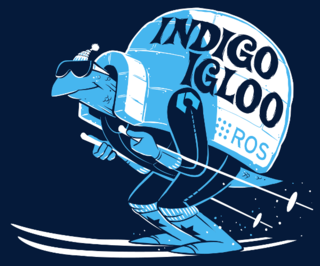
\includegraphics[height=35mm]{pictures/chapter2/indigo_igloo.png}
\caption{우분투 Trusty 버전과 ROS Indigo 버전의 로고}
\end{figure}

%-------------------------------------------------------------------------------
\subsection{ROS Indigo 설치 방법}\index{ROS Indigo 설치 방법}
\label{sec:ROSInstallation}

\begin{exercise}[간단 설치]
아래의 강좌보다 간단히 설치 할 수 있는 스크립트를 이용한 설치 방법은 섹션\ref{sec:SimpleInstallation}[ROS Indigo 간단 설치]을 참조하기 바란다.\\
\end{exercise}

%-------------------------------------------------------------------------------
\subsubsection{NTP (Network Time Protocol) 설정}
ROS 공식 설치 항목에는 포함되어 있지는 않지만 NTP 설정을 해주자.이는 서로 다른 PC간의 통신에서 ROS Time 의 오차를 줄일 수 있다. 설정법은 매우 간단하여 아래의 명령어처럼 우선 chrony 를 설치한 후, ntpdate 이라는 명렁어로 ntp 서버를 지정하면 된다. 결과, 서버측과의 현재 컴퓨터 시간 오차를 표시해주며, 설정한 서버 시간에 맞추게 될 것이다. 이는 서로 다른 PC 간에 같은 NTP 서버를 지정함으로써 시간 오차를 최소한으로 줄이는 방법이라 할 수 있다.
\\
\begin{lstlisting}[language=ROS]
$ sudo apt-get install chrony
$ sudo ntpdate ntp.ubuntu.com
\end{lstlisting}

%-------------------------------------------------------------------------------
\subsubsection{소스 리스트 추가}
sources.list 에 ROS 저장소 주소를 추가하자. 새로운 커맨드 창을 열고 아래와 같이 입력한다.
\\
\begin{lstlisting}[language=ROS]
$ sudo sh -c 'echo "deb http://packages.ros.org/ros/ubuntu trusty main" > /etc/apt/sources.list.d/ros-latest.list'
\end{lstlisting}

%-------------------------------------------------------------------------------
\subsubsection{키 설정}
ROS 저장소로부터 패키지를 다운로드 받기 위해 공개키를 추가하자. 아래와 같이 입력한다.
\\
\begin{lstlisting}[language=ROS]
$ wget https://raw.githubusercontent.com/ros/rosdistro/master/ros.key -O - | sudo apt-key add -
\end{lstlisting}

%-------------------------------------------------------------------------------
\subsubsection{패키지 인덱스 업데이트}
소스 리스트에 ROS 저장소 주소를 넣었으니 패키지 리스트를 다시 재인덱싱을 하고, 설치에 있어서 필수 사항은 아니지만 ROS 설치 전에 현재 설치된 우분투 관련 모든 패키지를 판올림 하기를 추천한다.
\\
\begin{lstlisting}[language=ROS]
$ sudo apt-get update && sudo apt-get upgrade
\end{lstlisting}

%-------------------------------------------------------------------------------
\subsubsection{ROS Indigo Igloo 설치}
이 명령어로 데스크톱용 기본적인 ROS 패키지들을 설치하게 된다. 여기에는 ROS, rqt, rviz, 로봇 관련 라이브러리, 시뮬레이션, 네이게이션 등이 포함되어 있다.
\\
\begin{lstlisting}[language=ROS]
$ sudo apt-get install ros-indigo-desktop-full
\end{lstlisting}

필자의 경우에는 추가로 rqt 관련 패키지를 설치하고 있다. 위의 설치만으로도 기본적인 rqt는 포함되지만 아래의 설치로 rqt관련 모든 패키지를 설치하는것이 여러모로 편하고, 다양한 rqt 플러그인을 사용가능해진다.
\\
\begin{lstlisting}[language=ROS]
$ sudo apt-get install ros-indigo-rqt-*
\end{lstlisting}

만약, 그 이외에 패키지를 설치하고 싶은 경우에는 아래와 같이 apt-cache 의 명령어를 이용하여 ros-indigo 로 시작되는 패키지들을 검색할 수 있다. 현재 아래의 명령어를 실행해보면 대략 900여개의 패키지를 확인할 수 있다. 패키지 개별 설치를 원하는 경우에는 sudo apt-get install ros-indigo-[패키지이름] 과 같은 명령어로 개별 패키지를 설치 가능하다. 그 이외에 GUI 툴인 sysnaptic package manager 를 이용해도 된다.

\begin{exercise}[APT (Advanced Packaging Tool)]
apt-get, apt-key, apt-cache 등에 나오는 apt는 Advanced Packaging Tool 이라고 하여서 우분투(Ubuntu)를 포함안 데비안(Debian)계열의 리눅스에서 많이 사용하는 패키지 관리 명령어이다\footnote{\url{http://en.wikipedia.org/wiki/Advanced_Packaging_Tool}}.
\end{exercise}

\begin{exercise}[패키지 검색 방법]
apt-cache search ros-indigo
\end{exercise}

\begin{exercise}[패키지 개별 설치 방법]
sudo apt-get install ros-indigo-패키지이름
\end{exercise}

\begin{exercise}[이전 버전의 ROS 삭제 및 번갈아 가며 사용하기]
아래의 명령어로 설정과 파일을 같이 삭제 가능하다. 만약, 기존 버전과 함께 사용하고자하는 경우에는 설정파일을 불러오는 명령어중 source /opt/ros/indigo/setup.bash 의 부분을 indigo 또는 hydro 로 바꾸면 된다. sudo apt-get purge ros-hydro-*
\end{exercise}

%-------------------------------------------------------------------------------
\subsubsection{rosdep 초기화}
ROS를 사용하기 전에 rosdep 를 초기화해주어야만 한다. rosdep 는 ros의 핵심 컴포넌트들을 사용하거나 컴파일 할때 의존성 패키지를 쉽게 설치하여 사용자 편의성을 높인 기능이다.
\\
\begin{lstlisting}[language=ROS]
$ sudo rosdep init
$ rosdep update
\end{lstlisting}

%-------------------------------------------------------------------------------
\subsubsection{rosinstall 설치}
ROS의 다양한 패키지를 인스톨하는 프로그램이다. 빈번하게 사용할 정도로 유용한 도구인 만큼 꼭 설치하자. 
\\
\begin{lstlisting}[language=ROS]
$ sudo apt-get install python-rosinstall
\end{lstlisting}

%-------------------------------------------------------------------------------
\subsubsection{환경설정 파일 불러오기}
환경 설정이 설정되어 있는 파일을 불러온다. ROS\_ROOT, ROS\_PACKAGE\_PATH 등의 환경 변수들이 정의되어 있다.
\\
\begin{lstlisting}[language=ROS]
$ source /opt/ros/indigo/setup.bash
\end{lstlisting}

%-------------------------------------------------------------------------------
\subsubsection{작업폴더 생성 및 초기화}
ROS에서는 catkin 이라는 ROS 전용 빌드 시스템을 사용하고 있다. 이를 사용하기 위해서는 아래와 같이 catkin 작업 폴더 및 작업 폴더 초기화 설정을 해주어야 한다. (아래의 설정은 ROS를 사용함에 있어서 처음 한 번만 해주면 된다.)
\\
\begin{lstlisting}[language=ROS]
$ mkdir -p ~/catkin_ws/src
$ cd ~/catkin_ws/src
$ catkin_init_workspace
\end{lstlisting}

catkin 작업 폴더를 생성하였으면 컴파일을 하자. 현재의 catkin 작업 폴더에는 src 폴더 및 그 안의 CMakeLists.txt 이외에 아무런 파일이 없지만 시험삼아 아래와 같이 catking\_make 명령어를 이용하여 빌드하여 보자. 
\\
\begin{lstlisting}[language=ROS]
$ cd ~/catkin_ws/
$ catkin_make
\end{lstlisting}

문제없이 빌드를 마치게 되면 아래와 같이 ls 명령어를 실행해보자. 유저가 직접 생성하였던 src 폴더 이외의 없었던 build 및 devel 폴더가 새로 생성되었을 것이다. catkin 빌드 시스템의 빌드 관련 파일은 build 폴더에, 빌드 후 실행관련 파일은 devel 폴더에 저장된다.
\\
\begin{lstlisting}[language=ROS]
$ ls
build  devel  src
\end{lstlisting}

마지막으로, catkin 빌드 시스템과 관련된 환경 파일을 불러오자. 
\\
\begin{lstlisting}[language=ROS]
$ source ~/catkin_ws/devel/setup.bash
\end{lstlisting}

%-------------------------------------------------------------------------------
\subsection{테스트}\index{테스트}

ROS의 모든 설치가 완료되었다. 마지막으로, 제대로 설치가 되었는지 테스트하기 위하여 지금의 모든 터미널창을 닫고, 새 터미널 창을 실행하자. 그 다음 아래의 명령어를 입력하여 roscore 를 실행해보자.
\\
\begin{lstlisting}[language=ROS]
$ roscore
\end{lstlisting}

\noindent
아래와 같이 에러가 없이 실행되었다면 설치가 완료된 것이다. 종료는 Ctrl-c 이다.
\\
\begin{lstlisting}[language=ROS]
... logging to /home/xxx/.ros/log/35c1e494-8097-11e4-a84a-d43d7e970cb0/roslaunch-xxx-23589.log
Checking log directory for disk usage. This may take awhile.
Press Ctrl-C to interrupt
Done checking log file disk usage. Usage is <1GB.

started roslaunch server http://192.168.4.100:51518/
ros_comm version 1.11.9


SUMMARY
========

PARAMETERS
 * /rosdistro: indigo
 * /rosversion: 1.11.9

NODES

auto-starting new master
process[master]: started with pid [23601]
ROS_MASTER_URI=http://192.168.4.100:11311/

setting /run_id to 35c1e494-8097-11e4-a84a-d43d7e970cb0
process[rosout-1]: started with pid [23614]
started core service [/rosout]
\end{lstlisting}

%-------------------------------------------------------------------------------
\section{ROS Indigo 간단 설치}\index{ROS Indigo 간단 설치}
\label{sec:SimpleInstallation}

자신이 사용중인 우분투 버전이 13.04, 14.04 이라면 앞서 설명한 ROS 설치를 간단히 수행하는 스크립트를 만들어 두었다. 이를 이용하면 비교적 손쉽게 설치 할 수 있다.
\\
\begin{lstlisting}[language=ROS]
$ wget https://raw.githubusercontent.com/oroca/oroca-ros-pkg/master/ros_indigo_install.sh
$ sh ros_indigo_install.sh
\end{lstlisting}

%-------------------------------------------------------------------------------
\section{ROS Indigo 설치 (간략버전)}\index{ROS Indigo 설치 (간략버전)}

아래의 명령어들은 챕터\ref{sec:ROSInstallation} ROS의 Indigo 버전 설치의 요약판이다. 긴 설명 없이 바로 설치하실 분들에게 도움이 될 것이다. ※ xxx.xxx.xxx.xxx 는 자신의 IP 주소를 입력하면 된다.

\begin{lstlisting}[language=ROS]
$ sudo apt-get install chrony
$ sudo ntpdate ntp.ubuntu.com
$ sudo sh -c 'echo "deb http://packages.ros.org/ros/ubuntu trusty main" > /etc/apt/sources.list.d/ros-latest.list'
$ wget https://raw.githubusercontent.com/ros/rosdistro/master/ros.key -O - | sudo apt-key add -
$ sudo apt-get update
$ sudo apt-get upgrade
$ sudo apt-get install ros-indigo-desktop-full
$ sudo apt-get install ros-indigo-rqt-*
$ sudo rosdep init
$ rosdep update
$ echo "source /opt/ros/indigo/setup.bash" >> ~/.bashrc
$ source ~/.bashrc
$ sudo apt-get install python-rosinstall
$ mkdir -p ~/catkin_ws/src
$ cd ~/catkin_ws/src
$ catkin_init_workspace
$ cd ~/catkin_ws/
$ catkin_make
$ echo "source ~/catkin_ws/devel/setup.bash" >> ~/.bashrc
$ echo "export ROS_MASTER_URI=http://xxx.xxx.xxx.xxx:11311" >> ~/.bashrc
$ echo "export ROS_HOSTNAME=xxx.xxx.xxx.xxx" >> ~/.bashrc
$ source ~/.bashrc
\end{lstlisting}

%-------------------------------------------------------------------------------
\section{ROS 개발 환경 구축 (환경설정)}\index{ROS 개발 환경 구축 (환경설정)}

%-------------------------------------------------------------------------------
\subsection{환경 설정}\index{환경 설정}

ROS 설치 과정에서 사용된 다음 명렁어처럼 환경 설정 파일을 불러오는 것은 새로운 터미널 창을 열때마다 매번 실행 해줘야 한다. 이러한 번거로운 작업을 없애기 위하여 새로운 터미널 창을 열때마다 정해진 환경 설정 파일을 읽어오도록 설정해주도록 하자. 그 이외에도 ROS 네트워크 설정 및 자주 사용하는 명령어를 단축 명령어도 설정하도록 하자.
\\
\begin{lstlisting}[language=ROS]
$ source /opt/ros/indigo/setup.bash
$ source ~/catkin_ws/devel/setup.bash
\end{lstlisting}

우선, gedit 프로그램과 같은 문서편집 프로그램을 사용하여 bashrc 파일을 수정하도록 하자. 아래의 명령어로 bashrc 파일을 불러오자. 이 책에서는 모든 챕터에 걸쳐서 문서폅집에 gedit을 사용하였지만 gedit가 아니더라도 sublime text, vim, emacs, nano 등을 사용해도 무방하다.
\\
\begin{lstlisting}[language=ROS]
$ gedit ~/.bashrc
\end{lstlisting}

bashrc 파일을 불러오면 이미 매우 많은 설정들이 있을 것이다. 이전 설정들은 건들지 말고, bashrc 파일의 제일 하단으로 내려가서 아래의 내용을 추가해주도록 하자. (xxx.xxx.xxx.xxx 는 자신의 IP이다.)
\\
\begin{lstlisting}[language=bash]
# Set ROS Indigo
source /opt/ros/indigo/setup.bash
source ~/catkin_ws/devel/setup.bash
# Set ROS Network
export ROS_MASTER_URI=http://xxx.xxx.xxx.xxx:11311
export ROS_HOSTNAME=xxx.xxx.xxx.xxx
# set ROS alias command
alias cw='cd ~/catkin_ws'
alias cs='cd ~/catkin_ws/src'
alias cm='cd ~/catkin_ws && catkin_make'
\end{lstlisting}

위 설정 이외에 필자는 아래와 같은 추가 설정을 하기도 한다. 아래의 내용은 어디까지나 참고 사항이니 설정하지 않아도 된다.
\\
\begin{lstlisting}[language=bash]
# Set User Alias
alias rm='rm -rf' 
alias eb='gedit ~/.bashrc' 
alias sb='source ~/.bashrc'
alias agi='sudo apt-get install'  
alias m='make -j4 -l4'  
alias gs='git status'  
alias gp='git pull'
alias catkin_eclipse='catkin_make --force-cmake -G"Eclipse CDT4 - Unix Makefiles"'
\end{lstlisting}

\noindent
다음으로는 위에서 설정한 내용들에 대하여 좀 더 자세히 설명하도록 하겠다.

%-------------------------------------------------------------------------------
\subsubsection{ROS 환경 설정 불러오기}
\# 은 주석문이 시작된다는 것을 알리는 문법이고 그 뒤의 내용이 주석문이다. 그리고, 2번째 줄의 source/opt/ros/indigo/setup.bash 및 3번째 줄의 source $\sim$/catkin\_ws/devel/setup.bash 은 필수로 설정해줘야 하는 ROS 환경 설정 파일이다.
\\
\begin{lstlisting}[language=bash]
# set ROS Indigo
source /opt/ros/indigo/setup.bash
source ~/catkin_ws/devel/setup.bash
\end{lstlisting}

%-------------------------------------------------------------------------------
\subsubsection{ROS 네트워크 설정}
ROS\_MASTER\_URI 와 ROS\_HOSTNAME 의 설정이다. ROS는 네트워크를 이용하여 노드간에 메시지 통신을하기 때문에 이 설정이 중요하다. 우선은 둘다 자신의 네트워크 IP를 입력해주면 된다. 차후에 마스터 PC가 따로 있고, 로봇은 호스트 PC를 사용하는 경우, 이를 구분하여 입력하면 서로 다른 컴퓨터간의 통신이 가능하게 된다. 지금은 둘다 모두 자신의 네트워크 IP를 입력해주자. 아래의 예제는 IP가 192.168.4.100 인 경우의 설정예이다. 
\\
\begin{lstlisting}[language=bash]
# set ROS Network
export ROS_MASTER_URI=http://192.168.4.100:11311
export ROS_HOSTNAME=192.168.4.100
\end{lstlisting}

\begin{exercise}[ifconfig]
리눅스에서 자신의 IP를 알아보는 방법으로는 ifconfig 명령어를 이용하는 방법이 제일 간단하다. 아래의 예제처럼 터미널창에서 ifconfig를 실행해보자. 유선이라면 eth, 무선이라면 wlan 의 항목의 inet addr 부분의 IP가 자신의 IP이다. 필자의 경우, 유선랜을 이용하지만 일부로 무선랜도 켜보았다. 아래의 예제에서의 유선 접속시의 IP는 192.168.4.100 이다.
\begin{lstlisting}[language=ROS, backgroundcolor=\color{ocre!10}, numbers=none]
$ ifconfig
eth0   Link encap:Ethernet  HWaddr xx:xx:xx:xx:xx:xx  
          inet addr:%*\textbf{\textcolor{red}{192.168.4.100}}*)  Bcast:192.168.4.255  Mask:255.255.255.0
          inet6 addr: fexx::d6xx:7exx:f1xx:xx2/64 Scope:Link

lo       Link encap:Local Loopback  
          inet addr:127.0.0.1  Mask:255.0.0.0
          inet6 addr: ::1/128 Scope:Host

wlan1 Link encap:Ethernet  HWaddr xx:xx:xx:xx:xx:xx
          inet addr:192.168.4.200  Bcast:192.168.4.255  Mask:255.255.255.0
          inet6 addr: fexx::23xx:dfxx:fexx:5exx/64 Scope:Link
\end{lstlisting}
\end{exercise}

%-------------------------------------------------------------------------------
\subsubsection{단축 명령어}
ROS 개발 작업에서 자주 사용하는 명령어를 단축 명령어로 설정하는 방법에 대해서 알아보도록 하자. 아래의 cw, cs, cm 은 필자가 만들어둔 단축 명령어이다. 이 단축 명령어는 리눅스에서 사용하는 alias 라는 단축 명령어를 이용하여 작성하였다.\\

\begin{itemize}[leftmargin=*]
\item cw 는 미리 설정해 둔 catkin 작업 폴더인 ~/catkin\_ws 로 이동한다. 
\item cs 는 catkin 작업 폴더 중 소스 파일이 담겨있는 ~/catkin\_ws/src 로 이동한다. 
\item cm 는 catkin 작업 폴더인 ~/catkin\_ws 로 이동한 후, catkin\_make 명령어로 ROS 패키지를 빌드하게 된다.
\end{itemize}

\vspace{\baselineskip}
\begin{lstlisting}[language=bash]
# set ROS alias command
alias cw='cd ~/catkin_ws'
alias cs='cd ~/catkin_ws/src'
alias cm='cd ~/catkin_ws && catkin_make'
\end{lstlisting}

\begin{exercise}[ROS 환경 설정 확인 방법]
아래처럼 export \textbar~grep ROS 명령어를 이용하여 자신이 현재 설정한 ROS 환경 설정들을 확인할 수 있다.
\begin{lstlisting}[language=bash, backgroundcolor=\color{ocre!10}, numbers=none]
$ export | grep ROS
declare -x ROSLISP_PACKAGE_DIRECTORIES="/home/xxx/catkin_ws/devel/share/common-lisp"
declare -x ROS_DISTRO="indigo"
declare -x ROS_ETC_DIR="/opt/ros/indigo/etc/ros"
declare -x ROS_HOSTNAME="192.168.4.100"
declare -x ROS_MASTER_URI="http://192.168.4.100:11311"
declare -x ROS_PACKAGE_PATH="/home/xxx/catkin_ws/src:/opt/ros/indigo/share:/opt/ros/indigo/stacks"
declare -x ROS_ROOT="/opt/ros/indigo/share/ros"
declare -x ROS_TEST_RESULTS_DIR="/home/xxx/catkin_ws/build/test_results"
\end{lstlisting}
\end{exercise}

%-------------------------------------------------------------------------------
\section{ROS 개발 환경 구축 (IDE)}\index{ROS 개발 환경 구축 (IDE)}

%-------------------------------------------------------------------------------
\subsection{통합 개발 환경 (Integrated Development Environment, IDE)}

IDE는 코딩, 디버그, 컴파일, 배포 등 프로그램 개발에 관련된 모든 작업을 하나의 프로그램 안에서 처리하는 환경을 제공하는 소프트웨어를 말한다. 아마 많은 개발자들이 자신만이 즐겨쓰는 IDE는 한두 개쯤은 있을 것으로 생각한다. 

ROS 또한 여러 IDE\footnote{ROS 위키, IDEs, \url{http://wiki.ros.org/IDEs}}를 사용할 수 있는데, 많이 사용되는 IDE로는 Eclipse, CodeBlocks, Emacs, Vim, NetBeans, QtCreator 등이 있다. 필자의 경우, 처음에는 Eclipse 를 사용 하였으나 Eclipse가 최근 버전에 와서는 매우 무겁게 느껴졌으며, ROS의 catkin 빌드 시스템 사용에 있어서 많은 불편을 느꼈다. 그래서, 다른 IDE 를 구축하고자 여러 IDE 를 검토해 봐다. 그 중 가장 적합한 툴로는 QtCreator\footnote{Qt Project, \url{http://qt-project.org/}}\footnote{Qt Download page, \url{http://qt-project.org/downloads}}가 아닐까 싶다. ROS 의 개발/디버깅 툴인 rqt 같은 경우나, RViz 같은 경우에도 Qt로 만들어져 있고, 사용자는 Qt 플러그인으로 기존 툴과 플러그인을 개발도 가능하다는 점에서 Qt의 편집기인 QtCreator 는 매우 유용하다고 볼 수 있다. 또한 Qt 를 이용하지 않더라도 범용적인 에디터로써의 기능도 충분히 갖추고 있을뿐 아니라, 프로젝트를 CMakeLists.txt 를 통하여 바로 불러올 수 있어서 catkin\_make 사용에 있어서 매우 편리하다.

아래의 내용은 QtCreator 로 ROS 개발 환경을 꾸미는 내용을 담고 있다. 반드시 QtCreator 를 이용하여 개발할 필요는 없으므로 QtCreator 를 IDE로 사용하지 않더라도 뒤에 따르는 내용을 이해하는 데에는 아무런 문제가 없음을 미리 밝혀둔다.

%-------------------------------------------------------------------------------
\subsubsection{QtCreator 설치}

\vspace{\baselineskip}
\begin{lstlisting}[language=ROS]
$ sudo apt-get install qtcreator
\end{lstlisting}

%-------------------------------------------------------------------------------
\subsubsection{QtCreator 구동}
QtCreator를 아이콘으로 실행시켜도 구동에는 문제 없으나 우리가 \textasciitilde/.bashrc 에 기술해둔 ROS 경로 등의 설정을 QtCreator 에도 적용하기 위해서는 새로운 터미널 창을 열어, 아래와 같이 실행해줘야 한다. 즉, QtCreator 를 실행할때 환경 설정 파일인 \textasciitilde/.bashrc 에 기술해 놓은 설정을 모두 적용하게 된다.\\

\begin{lstlisting}[language=ROS]
$ qtcreator
\end{lstlisting}

\noindent
위의 명령어로 아래와 같이 QtCreator 가 실행됨을 확인 할 수 있다.

\begin{figure}[h]
\centering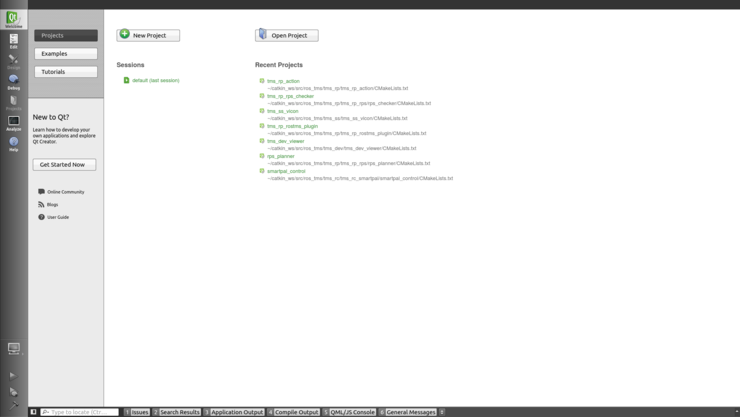
\includegraphics[width=0.9\columnwidth]{pictures/chapter2/qtcreator1.png}
\caption{QtCreator IDE}
\end{figure}

%-------------------------------------------------------------------------------
\subsubsection{ROS 패키지를 프로젝트로 불러오기}
앞서 말한바와 같이 QtCreator는 기본적으로 CMakeLists.txt 를 사용하고 있고, ROS 패키지도 CMakeLists.txt 기반이기에 단순히 아래와 화면의 OpenProject 버튼을 클릭하여 해당 ROS 패키지의 CMakeLists.txt 를 선택하면 손쉽게 프로젝트로 불러올 수 있다.

%-------------------------------------------------------------------------------
\subsubsection{ROS 패키지를 프로젝트로 불러오기}
컴파일의 경우에는 단순히 Ctrl + b 로 컴파일 하면 catkin\_make 가 실행된다. 단, 빌드 관련은 해당 패키지와 같은 위치의 폴더에 새로운 폴더로 생성된다. 예를 들어 tms\_rp\_action 이라는 패키지를 컴파일하면 build-tms\_rp\_action-Desktop-Default 이라는 폴더에 빌드 관련이 모두 놓이게 된다. 즉,  원래는 ~/catkin\_ws/build 와 ~/catkin\_ws/devel 에 보관되어야 할 파일들이 따로 컴파일 되어 새로운 장소에 놓이게 되므로 실행을 위해서는 나중에 다시 한번 catkin\_make 를 해줘야 한다. 이는 매번 해줄 필요는 없고 개발 도중에는 QtCreator 에서 개발, 디버깅한 후에 완료되어 실행할 때만 따로 catkin\_make 를 해주면 된다. 

\begin{figure}[h]
\centering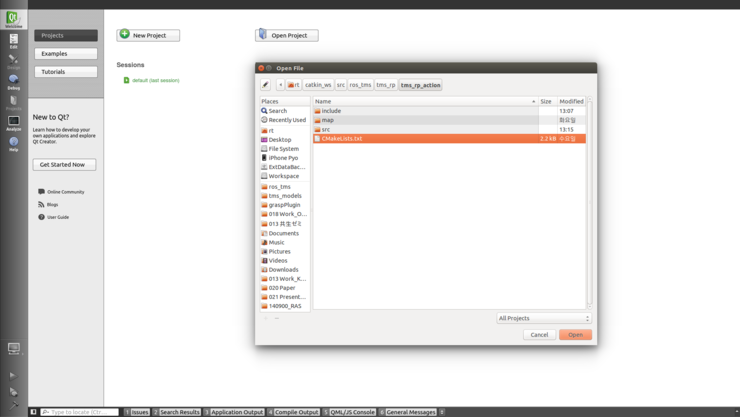
\includegraphics[width=0.9\columnwidth]{pictures/chapter2/qtcreator2.png}
\caption{QtCreator: 프로젝트 열기}
\end{figure}

\begin{figure}[h]
\centering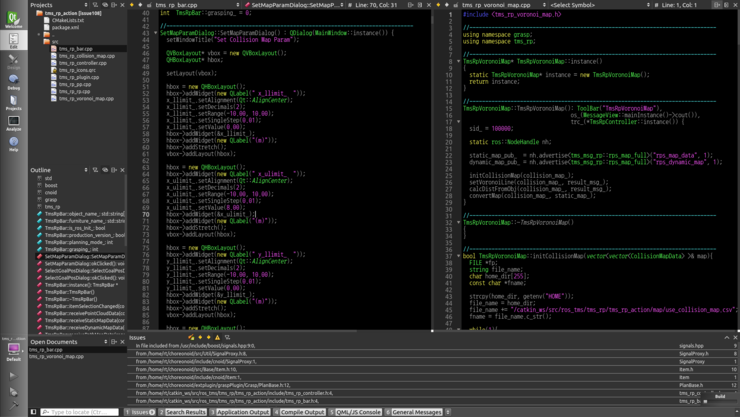
\includegraphics[width=0.9\columnwidth]{pictures/chapter2/qtcreator3.png}
\caption{QtCreator: 프로젝트 전개 모습}
\end{figure}

%-------------------------------------------------------------------------------
\section{ROS 동작 테스트}\index{ROS 동작 테스트}

%-------------------------------------------------------------------------------
\subsection{turtlesim 패키지}
일단, ROS를 설치하긴 했는데, 제대로 작동되는지 궁금하신분들을 위해 ROS에서 제공하는 간단한 예제 노드를 실행하는 방법에 대해 설명한다. 예제는 turtlesim 이라는 패캐지(노드의 묶음)로 ROS의 심볼인 거북이 모양을 한 로봇이 화면에 나타나고 키보드로 로봇의 이동을 간단히 조종해 보는 노드(프로그램)이다.

이번 내용부터는 노드(Node), 패키지(package), roscore 등 ROS 의 고유의 용어들이 많이 등장하는데 이번 강좌에서는 단순히 이런게 있구나 알아두기 바라며, 자세한 설명은 \textbf{섹션~\ref{sec:RosTerm}~\nameref{sec:RosTerm}(pp.\pageref{sec:RosTerm})} 에서 설명하도록 하겠다. 이번 강좌는 ROS 가 문제없이 설치됨을 확인정도 이기 때문에 본격적인 ROS 강좌가 들어가기 전에 몸풀기 운동 정도로 생각하자.

%-------------------------------------------------------------------------------
\subsection{roscore 실행}
새로운 터미널을 열어 다음과 같은 명렁어를 실행한다. 그러면 모든 ROS 시스템을 관할하는 roscore가 실행되게 된다.
\\
\begin{lstlisting}[language=ROS]
$ roscore
\end{lstlisting}

\begin{figure}[h]
\centering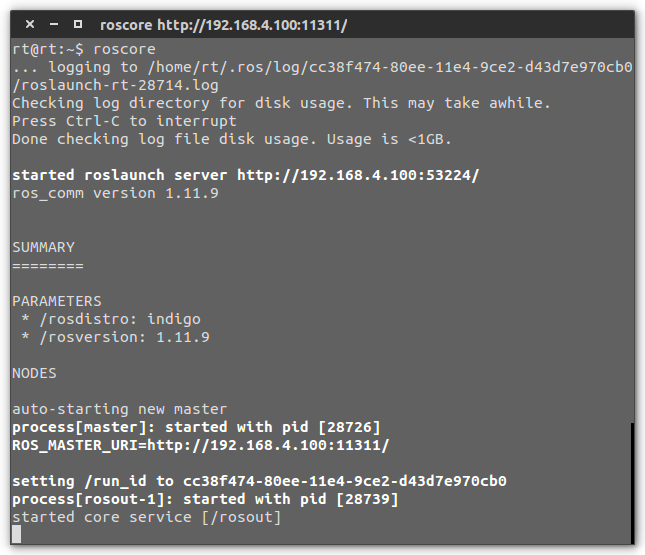
\includegraphics[width=0.7\columnwidth]{pictures/chapter2/roscore.png}
\caption{roscore가 실행된 화면}
\end{figure}

%-------------------------------------------------------------------------------
\subsection{turtlesim 패키지의 turtlesim\_node 실행}
새로운 터미널을 열어 다음과 같은 명렁어를 실행한다. 그러면 다음와 같은 메시지를 보게 되며, turtlesim 패키지의 turtlesim\_node 를 실행하게 된다. 별도의 창에 파란색 바탕의 화면에 거북이 한 마리가 보일 것이다. (거북이 모양은 실행에 따라 랜덤으로 바뀌기 때문에 필자의 모양과는 다를 수 있다.)
\\
\begin{lstlisting}[language=ROS]
$ rosrun turtlesim turtlesim_node
[ INFO] [1418273733.244561023]: Starting turtlesim with node name /turtlesim
[ INFO] [1418273733.249333831]: Spawning turtle [turtle1] at x=[5.544445], y=[5.544445], theta=[0.000000]
\end{lstlisting}

\begin{figure}[h]
\centering
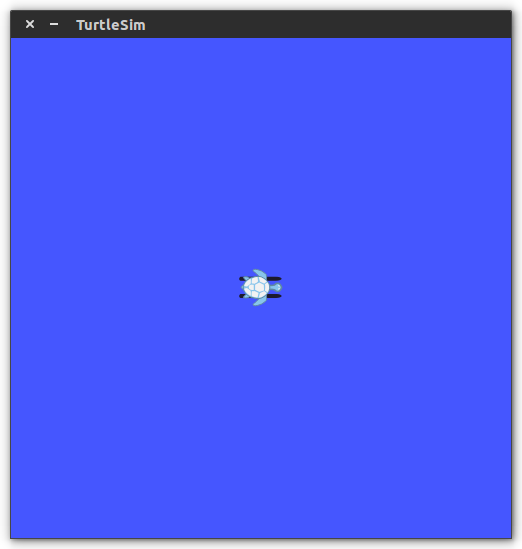
\includegraphics[width=0.49\columnwidth]{pictures/chapter2/turtlesim_node.png}
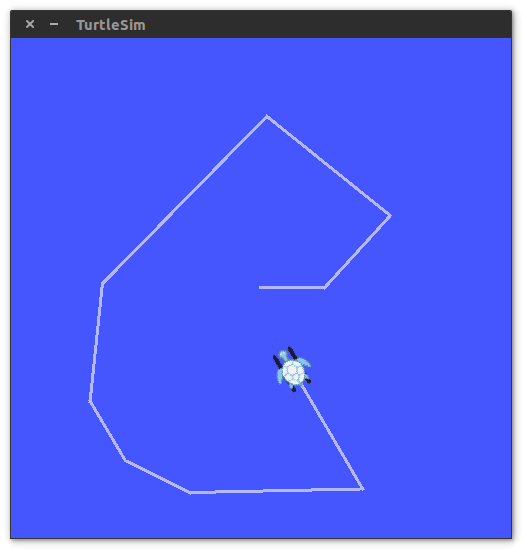
\includegraphics[width=0.49\columnwidth]{pictures/chapter2/turtlesim_node_move.png}
\caption{turtlesim\_node 노드를 실행하고 turtle\_teleop\_key 노드를 실행하여 화면위의 거북이를 이동시킨 모습}
\label{fig:turtlesim_node}
\end{figure}

%-------------------------------------------------------------------------------
\subsection{turtlesim 패키지의 turtle\_teleop\_key 실행}
새로운 터미널을 열어 다음과 같은 명렁어를 실행한다. 그러면 다음과 같은 메시지를 보게 되며, turtlesim 패키지의 turtle\_teleop\_key를 실행하게 된다. 이 \textbf{터미널 창 위}에서 키보드의 화살표(← → ↑ ↓)를 이용하여 그림\ref{fig:turtlesim_node}의 우측과 같이 거북이를 제어하게 된다. 간단하므로 직접 해보길 바란다. 제어하게 되면 화면 속의 거북이가 움직이게 되는데, 이는 간단히 시뮬레이션이지만 실제 로봇도 이와 같은 방법으로 원격조정이 가능하게 된다.
\\
\begin{lstlisting}[language=ROS]
$ rosrun turtlesim turtle_teleop_key
Reading from keyboard
---------------------------
Use arrow keys to move the turtle.
\end{lstlisting}

%-------------------------------------------------------------------------------
\subsection{rqt\_graph 패키지의 rqt\_graph 실행}
새로운 터미널을 열어 다음와 같은 명렁어를 실행한다. 그러면 rqt\_graph 패키지의 rqt\_graph 노드가 실행되게 된다. 그 결과 그림\ref{fig:turtlesim_node_graph} 같은 그래프를 볼 수 있을 것이다. 이는 현재 실행중인 노드(프로그램)들의 정보를 그래프로 볼 수 있는 노드이다.
\\
\begin{lstlisting}[language=ROS]
$ rosrun rqt_graph rqt_graph
\end{lstlisting}

rqt\_graph 노드는 현재 실행 중인 노드들의 정보를 볼 수 있는 GUI 형태의 노드이다. 동그라미는 노드를 의미하고, 네모는 토픽을 의미한다. 다음의 그림을 자세히 보자. /teleop\_turtle 노드로부터 화살표가 그어져 /turtlesim 으로 이어져 있다. 이는 두 노드가 실행 중 이고, 이 두 노드 간에는 메시지 통신이 이루어 지고 있다는 설명이다. 

그리고 화살표 사이의 네모박스 turtle1 토픽의 하위 토픽인 /turtle1/cmd\_vel 는 두 노드간의 토픽의 이름으로, teleop\_turtle 노드에서 키보드로 입력한 속도 명령이 turtlesim 으로 토픽을 통해 메세지(msg 데이타)가 송신되고 있다는 내용이다. 

즉, 위에서 실행한 두 노드를 이용하여 키보드 명령을 로봇 시뮬레이션에게 전달해 줬다는 내용이다. 자세한 내용은 추후 이어지는 내용에서 하도록 하고, 여기까지 진행이 원만히 되었다면, ROS 구동 테스트는 끝나게 된다.

\begin{figure}[h]
\centering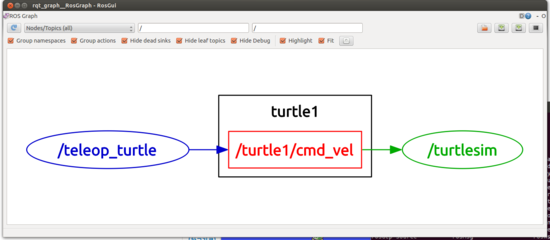
\includegraphics[width=0.8\columnwidth]{pictures/chapter2/turtlesim_node_graph.png}
\caption{노드들의 정보를 볼 수 있는 GUI 형태의 rqt\_graph 노드}
\label{fig:turtlesim_node_graph}
\end{figure}

%-------------------------------------------------------------------------------
\subsection{노드의 종료}

각각 실행된 roscore 및 노드는 터미널 창에서 Ctrl + c 를 눌러 종료한다.

%-------------------------------------------------------------------------------

% \chapterimage{chapter_head_1.pdf} % Chapter heading image

% \chapter{Presenting Information}

% \section{Table}\index{Table}

% \begin{table}[h]
% \centering
% \begin{tabular}{l l l}
% \toprule
% \textbf{Treatments} & \textbf{Response 1} & \textbf{Response 2}\\
% \midrule
% Treatment 1 & 0.0003262 & 0.562 \\
% Treatment 2 & 0.0015681 & 0.910 \\
% Treatment 3 & 0.0009271 & 0.296 \\
% \bottomrule
% \end{tabular}
% \caption{Table caption}
% \end{table}

% %-------------------------------------------------------------------------------

% \section{Figure}\index{Figure}

% \begin{figure}[h]
% \centering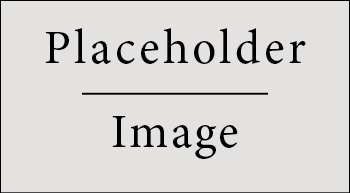
\includegraphics[scale=0.5]{placeholder}
% \caption{Figure caption}
% \end{figure}
% -*- root: main.tex -*-
%-------------------------------------------------------------------------------
\chapterimage{chapter_head_4.pdf} 

%-------------------------------------------------------------------------------
\chapter{ROS 개념 정리}

%-------------------------------------------------------------------------------
\section{ROS 용어 정리}\index{ROS 용어 정리}\label{sec:RosTerm}

ROS는 수 없이 많은 독특한 용어들이 사용된다. 여기에 많이 등장하는 ROS 용어들을 골라 정리하였다. ROS 용어 사전처럼 이용하면 좋을 듯 싶다. 대부분이 처음보는 용어일 수 있다. 이해가 안된다고 포기하지 말고 이해 안되는 부분은 일단 접어두고 내용으로 넘어가서 직접 실전을 통해 익힐 수 있도록 하자.

\vspace{\baselineskip}
\begin{definition}[ROS]\label{def:Ros}
ROS는 로봇 응용 프로그램을 개발을 위한 운영 체제와 같은 로봇 플랫폼이다. ROS는 로봇 응용프로그램을 개발할 때 필요한 하드웨어 추상화, 하위 디바이스 제어, 일반적으로 사용되는 기능의 구현, 프로세스간의 메시지 파싱, 패키지 관리, 개발환경에 필요한 라이브러리와 다양한 개발 및 디버깅 도구를 제공한다.
\end{definition}

\vspace{\baselineskip}
\begin{definition}[마스터(master)]\label{def:RosMaster}
마스터는 노드와 노드사이의 연결 및 메시지 통신을 위한 네임 서버와 같은 역할을 한다. roscore가 실행 명령어 이며, 마스터를 실행하면 각 노드들의 이름을 등록하고 필요에 따라 정보를 받을 수 있다. 마스터가 없이는 노드간의 접속, 토픽과 서비스와 같은 메시지 통신을 할 수 없다. 

마스터는 마스터에 접속하는 슬레이브들과의 접속 상태를 유지하지 않는 HTTP 기반의 프로토콜인 XMLRPC를 이용하여 슬레이브들과 통신하게 된다. 즉, 슬레이브인 노드들이 필요할때만 접속하여 자신의 정보를 등록하거나 다른 노드의 정보를 요청하여 수신받을 수 있다. 평상시에는 서로간의 접속 상태를 체크하지 않는다. 이러한 기능으로 매우 크고, 복잡한 환경에서도 적용 가능하다. 또한, XMLRPC는 매우 가볍고, 다양한 프로그래밍 언어를 지원하고 있기 때문에 다기종 하드웨어, 다언어를 지원하는 ROS에 매우 적합하다.

ROS를 구동하게 되면 사용자가 정해놓은 ROS\_MASTER\_URI 변수에 기재되어 있는 URI 주소 및 포트를 갖는다. 사용자가 설정해놓지 않은 경우에는 URI 주소로 현재의 로컬 IP 를 사용하고, 11311 포트를 이용하게 된다.
\end{definition}

\vspace{\baselineskip}
\begin{definition}[노드(node)]\label{def:RosNode}
ROS에서 최소 단위의 실행 프로세서를 가르키는 용어이다. 하나의 실행 가능한 프로그램으로 생각하면 된다. ROS에서는 하나의 목적에 하나의 노드를 작성하길 권하고 있으며 재사용이 쉽도록 구성하여 만들도록 권고하고 있다. 예를들어, 모바일 로봇의 경우, 로봇을 구동하기 위하여 각 프로그램을 세분화 시킨다. 예를들어, 센서 드라이브, 센서 데이타를 이용한 변환, 장애물 판단, 모터 구동, 엔코더 입력, 네이게이션 등 세부화된 작은 노드들을 이용한다.

노드는 생성과 함께 마스터에 노드이름, 발행자이름, 구독자이름, 토픽이름, 서비스이름, 메시지형태, URI 주소 및 포트를 등록한다. 이 정보들을 기반으로 각 노드는 노드끼리 토픽 및 서비스를 이용하여 메시지를 주고 받을 수 있다.

노드는 마스터와 통신할 때, XMLRPC를 이용하며, 노드간의 통신에서는 XMLRPC 및 TCP/IP 통신 계열의 TCPROS를 이용하고 있다. 노드간의 접속 요청 및 응답은  XMLRPC를 사용하며, 메시지 통신은 마스터와는 관계없이 노드와 노드간의 직접적인 통신으로 TCPROS를 이용하고 있다. URI 주소 및 포트는 현재 노드가 실행중인 컴퓨터에 저장된 ROS\_HOSTNAME 라는 환경 변수값을 URI 주소로 사용하며, 포트는 임의적 고유의 값으로 설정되게 된다.  
\end{definition}

\vspace{\baselineskip}
\begin{definition}[패키지(package)]\label{def:RosPackage}
ROS를 구성하는 기본 단위로써 실행 가능한 노드를 포함하고 있다. ROS는 패키지를 단위로 각각의 응용 프로그램들이 개발된다. 패키지는 최소한 하나 이상의 노드를 포함하고 있다. ROS Indio의 경우 공식적으로 약 970개 의 패키지를 제공하고 있으며, 유저들이 개발하여 공개된 패키지가 대략 3300개에 달하고 있다. 
\end{definition}

\vspace{\baselineskip}
\begin{definition}[메타패키지(metapackage)]\label{def:RosMetapackage}
공통된 목적을 가지는 패키지들을 모아둔 패키지들의 집합을 말한다. 복수의 패키지를 포함하고 있다.
\end{definition}

\vspace{\baselineskip}
\begin{definition}[메시지(message,msg)]\label{def:RosMessage}
노드는 메시지를 통해 노드간의 데이터를 주고받게 된다. 메시지는 integer, floating point, boolean 와 같은 변수 형태이다. 또한, 메시지안에 메시지를 품고 있는 간단한 데이터 구조 및 메시지들의 배열과 같은 구조도 사용할 수 있다. 

메세지를 이용한 통신방법으로는 TCPROS, UDPROS 방식등이 있으며, 단방향 메시지 송/수신 방식의 토픽과 양방향 메시지 요청/응답 방식의 서비스를 이용하고 있다.
\end{definition}

\vspace{\baselineskip}
\begin{definition}[토픽(topic)]\label{def:RosTopic}
토픽은 "이야깃거리"이다. 발행자 노드가 하나의 이야깃거리에서 대해서 토픽이라는 이름으로 마스터에 등록한 후, 이야깃거리에 대한 이야기를 메시지 형태로 발행한다. 이 이야깃거리를 수신 받기를 원하는 구독자 노드는 마스터에 등록된 토픽의 이름에 해당되는 발행자 노드의 정보를 받는다. 이 정보를 기반으로 구독자 노드는 발행자 노드와 직접적으로 연결하여 메시지를 송/수신 또는 요청/응답 받게 된다. 
\end{definition}

\vspace{\baselineskip}
\begin{definition}[발행(publish) 및 발행자(Publisher) ]\label{def:RosPublish}
발행은 토픽의 내용에 해당되는 메시지 형태의 데이터를 송신하는 것을 말한다. 발행자 노드는 발행을 수행하기 위하여 토픽을 포함한 자신의 정보들을 마스터에 등록하고, 구독을 원하는 구독자 노드에게 메시지를 보내게 된다. 발행자는 이를 실행하는 개체로써 노드에서 선언하게 된다. 발행자는 하나의 노드에서 복수로 선언이 가능하다.
\end{definition}

\vspace{\baselineskip}
\begin{definition}[구독(subscribe) 및 구독자(Subscriber)]\label{def:RosSubscribe}
구독은 토픽의 내용에 해당되는 메시지 형태의 데이터를 수신하는 것을 말한다. 구독자 노드는 구독을 수행하기 위하여 토픽을 포함한 자신의 정보들을 마스터에 등록하고, 구독하고자 하는 토픽을 발행하는 발행자 노드의 정보를 마스터로부터 받는다. 이 정보를 기반으로 구독자 노드는 발행자 노드와 직접적으로 접속하여 발행자 노드로부터 메시지를 받게 된다. 구독자는 이를 실행하는 개체로써 노드에서 선언하게 된다. 구독자는 하나의 노드에서 복수로 선언이 가능하다.
\end{definition}

\vspace{\baselineskip}
\begin{definition}[서비스(service)]\label{def:RosService}
발행과 구독 개념의 토픽 통신 방식은 비동기 방식이라 필요에 따라서 주어진 데이터를 전송하고 받기에 매우 훌륭한 방법이다. 또한, 한번의 접속으로 지속적인 메시지를 송/수신하기 때문에 지속적으로 메시지를 발송해야하는 센서 데이터에 적합하여 많이 사용되고 있다. 하지만, 경우에 따라서는 요청과 응답이 함께 사용되는 동기 방식의 메시지 교환 방식도 필요하다. 이에 따라, ROS에서는 서비스라는 이름으로 메시지 동기 방식을 제공하고 있다. 서비스는 요청이 있을 경우에 응답을 하는 서비스 서버와 요청을 하고 응답을 받는 서비스 클라이언트로 나뉘어 있다. 서비스는 토픽과는 달리 1회성 메시지 통신이다. 서비스의 요청과 응답이 완료되면 연결된 두 노드의 접속은 끊기게 된다. 
\end{definition}

\vspace{\baselineskip}
\begin{definition}[서비스 서버 (service server)]\label{def:RosServiceServer}
서비스 서버는 요청을 입력으로 받고, 응답을 출력으로 하는 서비스 메시지 통신의 서버 역할을 말한다. 요청과 응답은 모두 메시지로 되어 있으며, 서비스 요청에 의하여 주어진 서비스를 수행 후에 그 결과를 서비스 클라이언트에게 전달한다. 서비스 메시지 방식은 동기식이기에 정해진 명령을 지시 및 수행하는 노드에 사용하는 경우가 많다.
\end{definition}

\vspace{\baselineskip}
\begin{definition}[서비스 클라이언트 (service client)]\label{def:RosServiceClient}
서비스 클라이언트는 요청을 출력으로 하고, 응답을 입력으로 받는 서비스 메시지 통신의 클라이언트 역할을 말한다. 요청과 응답은 모두 메시지로 되어 있으며, 서비스 요청을 서비스 서버에 전달하고 그 결과 값을 서비스 서버로 부터 받는다. 서비스 메시지 방식은 동기식이기에 정해진 명령을 지시 및 수행하는 노드에 사용하는 경우가 많다.
\end{definition}

\vspace{\baselineskip}
\begin{definition}[캐킨(catkin)]\label{def:RosCatkin}
ROS의 빌드 시스템을 말한다. ROS의 빌드 시스템은 기본적으로 CMake(Cross Platform Make) 를 이용하고 있어서 패키지 폴더에 CMakeLists.txt 라는 파일에 빌드 환경을 기술하고 있다. ROS에서는 CMake 를 ROS에 맞도록 수정하여 ROS에 특화된 캐킨 빌드 시스템을 만들었다. 캐킨 빌드 시스템은 ROS와 관련된 빌드, 패키지 관리, 패키지간의 의존관계 등을 편리하게 사용할 수 있도록 하고 있다. 
\end{definition}

\vspace{\baselineskip}
\begin{definition}[ROS빌드(rosbuild)]\label{def:RosRosbuild}
catkin 빌드 시스템의 이전에 사용되었던 빌드 시스템이다. ROS Fuerte 버전부터 rosbuild 빌드 시스템 대신에 catkin 빌드 시스템을 사용하고 있으나, rosbuild 빌드 시스템 또한 사용 가능하다. 하지만, 이는 ROS 버전의 호환성을 위해 남겨둔 것이지 공식적으로는 추천하지 않는다. 만약, rosbuild 빌드 시스템을 사용한 이전 패키지를 사용해야만 한다면 rosbuild를 catkin으로 변경하여 사용하기를 추천한다. 
\end{definition}

\vspace{\baselineskip}
\begin{definition}[ROS코어(roscore)]\label{def:RosCore}
ROS 마스터를 구동하는 명령어이다. 같은 네트웍이라면 다른 컴퓨터에서 실행하여도 된다. 단, 멀티 ROS코어를 지원하는 특수한 경우를 제외하고는 ROS코어는 동일 네트워크에서 하나만 구동되게 디노다. ROS를 구동하게 되면 사용자가 정해놓은 ROS\_MASTER\_URI 변수에 기재되어 있는 URI 주소 및 포트를 갖는다. 사용자가 설정해놓지 않은 경우에는 URI 주소로 현재의 로컬 IP 를 사용하고, 11311 포트를 이용하게 된다.
\end{definition}

\vspace{\baselineskip}
\begin{definition}[매개변수(parameter)]\label{def:RosParameter}
노드에서 사용되는 매개변수를 말한다. 흔히, 윈도우즈 프로그램에서 *.ini 설정파일과 같다고 생각하면 된다. 디폴트로 설정 값들이 지정되어 있고, 필요에 의해서 외부에서 이 매개변수를 읽기, 쓰기가 가능하다. 특히, 상황에 맞추어 이 매개변수를 외부에서 쓰기기능을 이용하여 설정값을 실시간으로 바꿀수 있기에 매우 유용한 방법이다. 예를들어 접속하는 USB포트 및 카메라 캘리브레이션 값, 속도 및 명령어들의 최대/최저 값 등의 설정등을 지정할 수 있다.
\end{definition}

\vspace{\baselineskip}
\begin{definition}[매개변수 서버(parameter server)]\label{def:RosParameterServer}
매개변수 서버는 패키지에서 매개변수를 사용할 때, 각 매개변수를 등록하는 서버를 말한다. 매개변수 서버는 마스터의 일부분이다. 
\end{definition}

\vspace{\baselineskip}
\begin{definition}[rosrun]\label{def:RosRun}
ROS의 기본적인 실행 명령어이다. 패키지에서 하나의 노드를 실행하는데 사용된다. 노드가 사용하는 URI 주소 및 포트는 현재 노드가 실행중인 컴퓨터에 저장된 ROS\_HOSTNAME 라는 환경 변수값을 URI 주소로 사용하며, 포트는 임의적 고유의 값으로 설정되게 된다.
\end{definition}

\vspace{\baselineskip}
\begin{definition}[roslaunch]\label{def:RosLaunch}
rosrun이 하나의 노드를 실행하는 명령어라면 ROS런치(roslaunch)는 복 수개의 노드를 실행하는 개념이다. 이 명령어를 통해 정해진 단일 혹은 복수의 노드를 실행시킬 수 있다. 

그 이외의 기능으로 실행시에 패키지의 매개변수를 변경, 노드 명의 변경, 노드 네임 스페이스 설정, ROS\_ROOT 및 ROS\_PACKAGE\_PATH 설정, 이름 변경, 환경 변수 변경 등의 실행시 변경할 수 있는 많은 옵션들을 갖춘 노드 실행에 특화된 ROS 명령어이다. 

ROS런치는 *.launch 라는 ROS런치파일을 사용하여 실행 노드에 대한 설정을 해주는데 이는 XML 기반으로 되어 있으며, 태그별 옵션을 제공하고 있다.
\end{definition}

\vspace{\baselineskip}
\begin{definition}[배그(bag)]\label{def:RosBag}
ROS에서 주고받는 메시지의 데이터를 저장할 수 있는 있는데 이를 배그라고 한다. ROS에서는 이 배그를 이용하여 메시지를 저장하고 필요로 할 때 이를 재생하여 이전 상황을 그대로 재현할 수있는 기능을 갖추고 있다. 예를들어, 센서를 이용한 로봇 실험을 실행할 때, 센서 값을 배그를 이용하여 메시지 형태로 저장한다. 이 저장된 메시지는 같은 실험을 수행하지 않아도 저장해둔 배그 파일을 재생하는 것으로 그 당시의 센서값을 반복 사용가능하다. 특히, 기록, 재생의 기능을 활용하여 반복되는 프로그램 수정이 많은 알고리즘 개발에 매우 유용하다. 
\end{definition}

\vspace{\baselineskip}
\begin{definition}[ROS Wiki]\label{def:RosWiki}
ROS의 각 패키지 및 기능들을 설명하는 페이지(\url{http://wiki.ros.org/})이다. 각 패키지는 위키 페이지에 패키지에 대한 간단한 설명, 사용되는 매개변수, 저작자, 라이선스, 홈페이지, 저장소, 튜토리얼등을 기술하고 있다.
\end{definition}

\vspace{\baselineskip}
\begin{definition}[저장소(repositoy)]\label{def:RosRepository}
공개된 패키지의 경우, 각 패키지의 위키에 저장소를 명시하고 있다. 저장소는 패키지가 저장된 웹상의 저장소 URL 주소이며 svn, hg, git 등의 소스 관리 시스템을 이용하여 이슈, 개발, 다운로드 등을 관리하고 있다.
\end{definition}

\vspace{\baselineskip}
\begin{definition}[그래프(graph)]\label{def:RosGraph}
위에서 설명한 노드, 토픽, 발행자, 구독자 관계를 그래프를 통해 나타나게 하는 것이다. 현재 실행중인 메시지 통신을 그래프화 시킨 것으로 1회성 서비스에 대한 그래프는 작성할 수 없다. 실행은 rqt\_graph 패키지의 rqt\_graph 노드를 실행하면 된다. 실행 명령에는 두 가지가 있는데 rqt\_graph과 rosrun rqt\_graph rqt\_graph 이다.   
\end{definition}

\vspace{\baselineskip}
\begin{definition}[이름(name)]\label{def:RosName}
노드, 매개변수, 토픽, 서비스는 모두 이름을 갖고 있다. 이 이름은 마스터에 등록하고 각 노드의 매개변수, 토픽, 서비스를 사용할때 이 이름을 기반으로 상호적으로 동작하도록 되어있다. 또한, 이름은 실행시에 변경가능하기 때문에 매우 유연하고, 같은 노드, 매개변수, 토픽, 서비스라고 하여도 다른 이름으로 중복 실행이 가능하다. 이러한 이름의 사용으로 ROS는 큰 규모의 프로젝트, 복잡한 구조의 시스템에도 적합하다.  
\end{definition}

\vspace{\baselineskip}
\begin{definition}[클라이언트 라이브러리(client libray)]\label{def:RosClientLibray}
ROS는 사용되는 언어의 의존성을 낮추기 위하여 클라이언트 라이브러리라는 이름으로 각종 언어의 개발환경을 제공하고 있다. 주요한 클라이언트 라이브러리로는 C++, Python, Lisp 등이 있으며, 그 이외에도 java, lua, .NET, EusLisp, R 등의 언어들을 사용가능하다. 이를 위해 roscpp, rospy, roslisp, rosjava, roslua, roscs, roseus, PhaROS, rosR 등의 클라이언트 라이브러리가 개발되었다.
\end{definition}

\vspace{\baselineskip}
\begin{definition}[URI (Uniform Resource Identifier)]\label{def:RosURI}
URI (Uniform Resource Identifier, 통합 자원 식별자) 는 인터넷에 있는 자원을 나타내는 유일한 주소이다. URI 은 인터넷에서 요구되는 기본조건으로서 인터넷 프로토콜에서 식별자로 사용된다.
\end{definition}

\vspace{\baselineskip}
\begin{definition}[MD5 (Message-Digest algorithm 5)]\label{def:RosMD5}
MD5는 128비트 암호화 해시 함수이다. 주로 프로그램이나 파일이 원본 그대로인지를 확인하는 무결성 검사 등에 사용된다. ROS에서의 메시지를 이용한 통신에서 MD5를 이용하여 메시지 송수신의 무결성 검사를 하고 있다.
\end{definition}

\vspace{\baselineskip}
\begin{definition}[RPC(Remote Procedure Call)]\label{def:RosRPC}
RPC란 '멀리 떨어져(Remote) 있는 컴퓨터상의 프로그램이 다른 컴퓨터 내에 있는 서브프로그램(Procedure)을 불러내는(Call)' 것을 의미한다. 컴퓨터 프로그램이 다른 주소 공간에서 원격 제어를 위한 프로그래머의 세세한 코딩 없이 함수나 프로시저의 실행을 허용하는 기술로써 대표적으로는 TCP/IP, IPX 등의 전송 프로토콜을 이용한다. 
\end{definition}

\vspace{\baselineskip}
\begin{definition}[XML(Extensible Markup Language)]\label{def:RosXML}
XML은 W3C에서 다른 특수 목적의 마크업 언어를 만드는 용도에서 권장되는 다목적 마크업 언어(markup language)로 태그 등을 이용하여 데이터의 구조를 명기하는 언어의 한 가지이다. 
\end{definition}

\vspace{\baselineskip}
\begin{definition}[XMLRPC]\label{def:RosXMLRPC}
XML-RPC란, RPC 프로토콜의 일종으로서, 인코딩 형식에서는 XML을 채택하고, 전송 방식에서는 접속 상태를 유지하지 않고 체크하지 않는 요청/응답 방식의 HTTP 프로토콜을 사용하고 있다. XML-RPC는 매우 단순한 규약으로서, 작은 데이터 형식이나 명령을 정의하는 정도로만 사용하고 있어서 꽤나 단순한 편이다. 이러한 특징으로, XMLRPC는 매우 가볍고, 다양한 프로그래밍 언어를 지원하고 있기 때문에 다기종 하드웨어, 다언어를 지원하는 ROS에 매우 적합하다.
\end{definition}

\vspace{\baselineskip}
\begin{definition}[TCP/IP (Transmission Control Protocol / Internet Protocol)]\label{def:RosTCPIP}
TCP 는 Transmission Control Protocol 의 약자로써, 전송 제어 프로토콜이라고 부른다. 흔히 TCP/IP 라 부르는데 이는 인터넷 프로토콜 계층의 시각에서 보면 IP(Internet Protocol) 를 기반으로 전송 제어 프로토콜인 TCP 를 사용하여 데이터의 전달을 보증하고 보낸 순서대로 송/수신하게 된다. 
\end{definition}

\vspace{\baselineskip}
\begin{definition}[TCPROS]\label{def:RosTCPROS}
메시지 및 서비스에서 사용되는 TCP/IP 기반의 메시지 방식을 TCPROS라고 한다.
\end{definition}

\vspace{\baselineskip}
\begin{definition}[UDPROS]\label{def:RosUDPROS}
메시지 및 서비스에서 사용되는 UDP 기반의 메시지 방식을 UDPROS라고 한다. 일반적으로 ROS에서는 사용되지 않고 있다.
\end{definition}

\vspace{\baselineskip}
\begin{definition}[CMakeLists.txt]\label{def:RosCMakeLists.txt}
ROS의 빌드 시스템인 캐킨은 기본적으로 CMake를 이용하고 있어서 패키지 폴더에 CMakeLists.txt 라는 파일에 빌드 환경을 기술하고 있다.
\end{definition}

\vspace{\baselineskip}
\begin{definition}[package.xml]\label{def:RosPackage.XML}
패키지의 정보를 담은 XML 파일로써 패키지의 이름, 저작자, 라이선스, 의존성 패키지 등을 기술하고 있다.
\end{definition}

\newpage
%-------------------------------------------------------------------------------
\section{ROS 개념 정리}\index{ROS 개념 정리}

%-------------------------------------------------------------------------------
\subsection{메시지 통신}\index{메시지 통신}

지금까지 ROS에 대해서 설명하였지만, 실제로 어떻게 동작하는 것인지에 대해서는 자세히 언급하지 않았었다. 이번 강좌에서는 ROS의 동작에 대한 핵심 기능 및 개념에 대해서 설명하려고 한다. ROS는 매우 생소한 용어들이 많이 등장하므로 \textbf{섹션~\ref{sec:RosTerm}~\nameref{sec:RosTerm}(pp.\pageref{sec:RosTerm})}를 참고하면서 ROS 개념을 이해하면 좋을 듯 싶다. ROS 개념 설명에서 사용되는 각 용어들의 상세한 설명은 용어 정리 강좌를 참조하기 바라며, 이번 강좌에서는 개념만을 설명하도록 하겠다.

ROS의 핵심 개념은 노드간의 메시지 통신\footnote{ROS Wiki, Concepts, \url{http://wiki.ros.org/ROS/Concepts}}\footnote{ROS Wiki, Higher-Level Concepts, \url{http://wiki.ros.org/ROS/Higher-Level\%20Concepts}}이다. 목적에 따라 세분화된 최소 단위의 실행 프로그램인 노드는 다른 노드와 처리 결과 값을 주고 받게 됨으로써 하나의 커다란 프로그램이 된다. 이를 위하여 메시지 통신에는 단 방향으로 연속적으로 메시지를 송수신하는 토픽 메시지 통신과 쌍 방향으로 요청과 응답 형태의 정해진 작업을 수행하게 하는 목적의 서비스 메시지 통신이 있다. 

이러한 노드간의 메시지 통신에는 접속이 필요한데, 노드간의 접속을 돕는 것이 마스터\footnote{ROS Wiki, Master, \url{http://wiki.ros.org/Master}}이다. 마스터는 노드의 이름, 토픽 및 서비스의 이름, URI 주소와 포트, 매개변수 등의 네임 서버와 같은 역할을 하게된다. 즉, 노드는 생성과 동시에 마스터에 자신의 정보를 등록하게 되고, 다른 노드가 마스터를 통해 접속하려는 노드의 정보를 마스터로부터 취득한다. 그 후, 노드와 노드가 직접 접속하여 메시지 통신을 하는 것이다. 

이를 그림으로 나태내면 다음의 그림과 같다. 마스터는 노드들의 정보를 관리하며, 각 노드는 필요에 따라 다른 노드와 접속, 메시지 통신을 하게 된다. 여기서 우리는 가장 중요한 마스터, 노드, 토픽\footnote{ROS Wiki, Topics, \url{http://wiki.ros.org/Topics}}, 서비스\footnote{ROS Wiki, Services, \url{http://wiki.ros.org/Services}}, 메시지\footnote{ROS Wiki, Messages, \url{http://wiki.ros.org/Messages}}의 흐름에 대해서 알아보도록 하자.

\begin{figure}[h]
\centering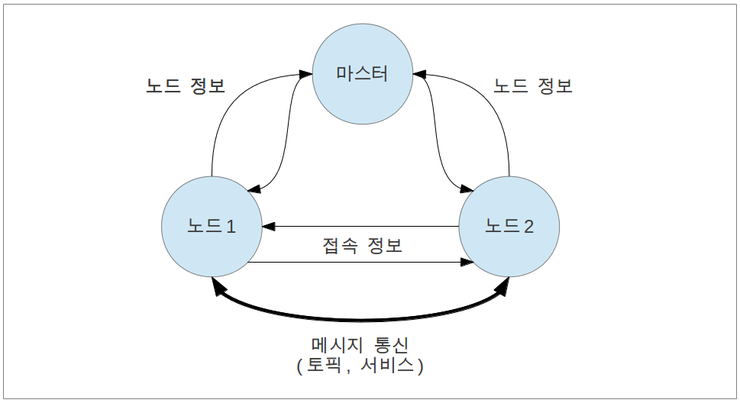
\includegraphics[width=\columnwidth]{pictures/chapter4/message_communication.png}
\caption{메시지 통신}
\end{figure}


%-------------------------------------------------------------------------------
\subsection{마스터 구동}\index{마스터 구동}

노드들간의 메시지 통신에서 연결 정보를 관리하는 마스터는 ROS를 사용하기 위해서 제일 먼저 구동해야하는 필수 요소이다. 다음과 같이 roscore라는 실행 명령어로 ROS 마스터는 구동되며, XMLRPC으로 서버를 구동하게 된다. 마스터는 노드간의 접속을 위하여 노드들의 이름, 토픽 및 서비스의 이름, 메시지 형태, URI 주소 및 포트를  등록받고, 요청이 있을 경우 이 정보를 다른 노드에게 알려주는 역할을 한다.

\begin{lstlisting}[language=ROS]
$ roscore
\end{lstlisting}

\begin{figure}[h]
\centering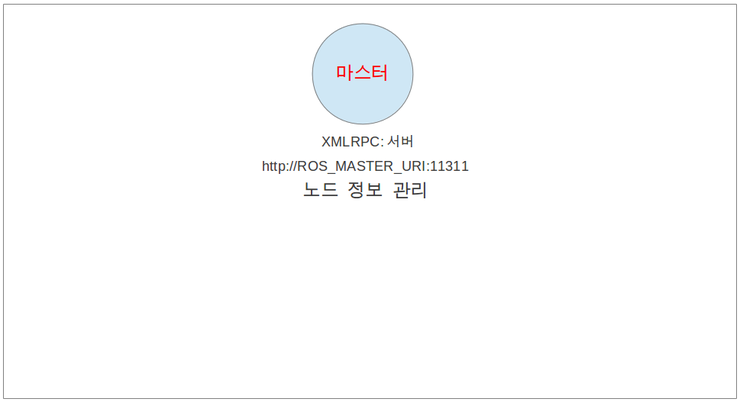
\includegraphics[width=0.7\columnwidth]{pictures/chapter4/notion1.png}
\caption{마스터 구동}
\end{figure}

%-------------------------------------------------------------------------------
\subsection{구독자 노드(Node) 구동}\index{구독자 노드(Node) 구동}
 
구독자 노드는 다음과 같이 rosrun 및 roslaunch 이라는 실행 명령어로 구동된다. 구독자 노드는 구동과 함께 마스터에 자신의 구독자노드이름, 토픽이름, 메시지형태, URI 주소 및 포트를 등록한다. 마스터와 노드는 XMLRPC 를 이용하여 통신하게 된다.

\begin{lstlisting}[language=ROS]
$ rosrun PACKAGE_NAME NODE_NAME
$ roslaunch PACKAGE_NAME LAUNCH_NAME
\end{lstlisting}

\begin{figure}[h]
\centering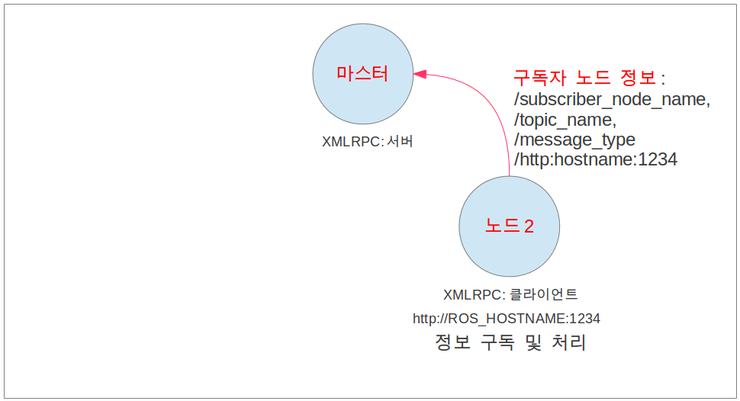
\includegraphics[width=0.7\columnwidth]{pictures/chapter4/notion2.png}
\caption{구독자 노드 구동}
\end{figure}

\newpage
%-------------------------------------------------------------------------------
\subsection{발행자 노드(Node) 구동}\index{발행자 노드(Node) 구동}

발행자 노드는 구독자 노드와 마찬가지로 rosrun 및 roslaunch 이라는 실행 명령어로 구동한다. 발행자 노드는 구동과 함께 마스터에 자신의 발행자노드이름, 토픽이름, 메시지형태, URI 주소 및 포트를 등록한다. 마스터와 노드는 XMLRPC 를 이용하여 통신하게 된다.

\begin{figure}[h]
\centering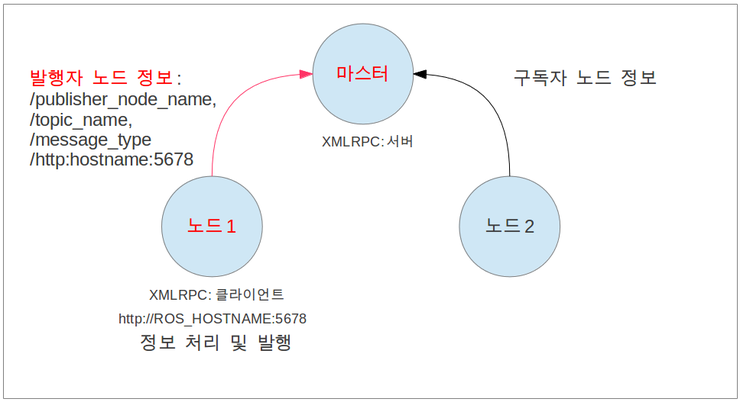
\includegraphics[width=0.9\columnwidth]{pictures/chapter4/notion3.png}
\caption{발행자 노드 구동}
\end{figure}

%-------------------------------------------------------------------------------
\subsection{발행자 정보 알림}\index{발행자 정보 알림}

마스터는 구독자 노드에게 접속하기 원하는 발행자의 이름, 주소등의 정보를 접속하고자하는 노드에게 알린다. 마스터와 노드는 XMLRPC 를 이용하여 통신하게 된다.

\begin{figure}[h]
\centering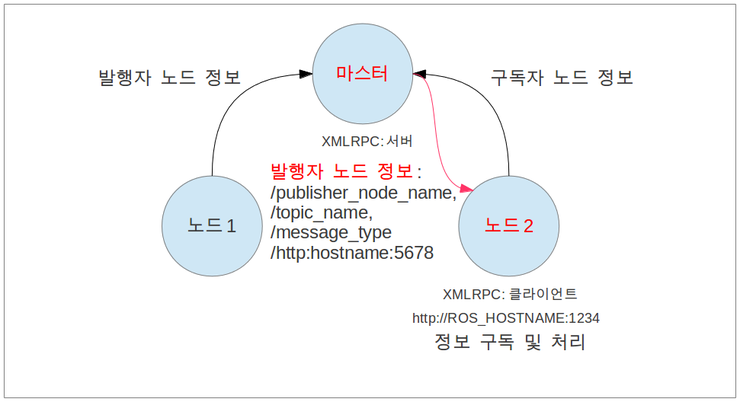
\includegraphics[width=0.9\columnwidth]{pictures/chapter4/notion4.png}
\caption{발행자 정보 알림}
\end{figure}

\newpage
%-------------------------------------------------------------------------------
\subsection{발행자 노드에 접속 요청}\index{발행자 노드에 접속 요청}

구독자 노드는 마스터로부터 받은 발행자 정보를 기반으로 발행자 노드에게 직접 접속 요청을 한다. 이때에 전송하는 정보로는 자신의 구독자 노드 이름, 토픽이름, 메시지방식(TCPROS 또는 UDPROS)이 있다. 발행자 노드와 구독자 노드는 XMLRPC 를 이용하여 통신하게 된다.

\begin{figure}[h]
\centering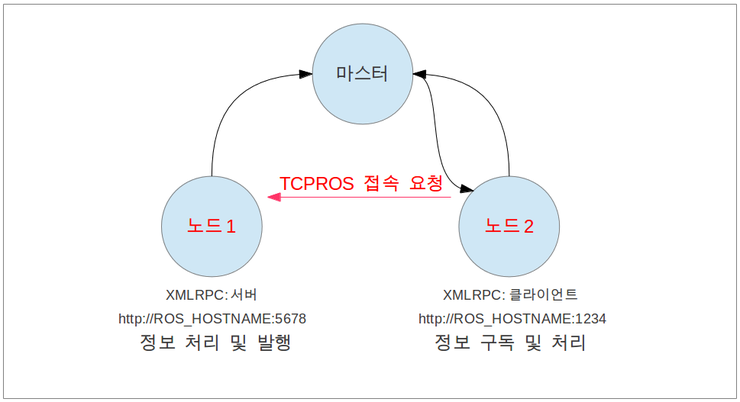
\includegraphics[width=0.9\columnwidth]{pictures/chapter4/notion5.png}
\caption{발행자 노드에 접속 요청}
\end{figure}

%-------------------------------------------------------------------------------
\subsection{발행자 노드에 접속 응답}\index{발행자 노드에 접속 응답}

발행자 노드는 구독자노드에게 접속 응답에 해당되는 자신의 TCP 서버의 정보인 URI주소와 포트를 전송한다. 발행자 노드와 구독자 노드는 XMLRPC 를 이용하여 통신하게 된다.

\begin{figure}[h]
\centering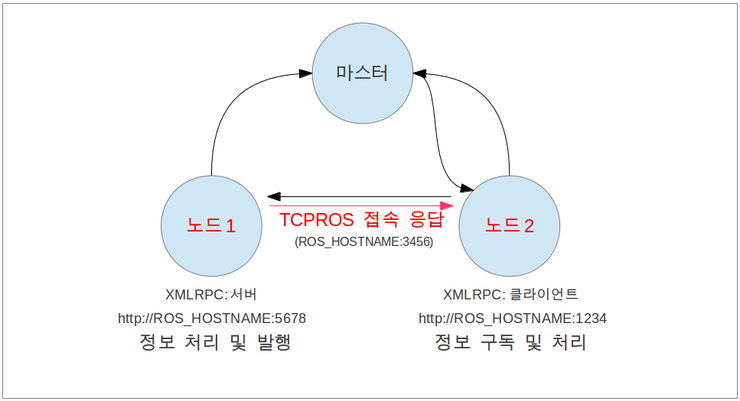
\includegraphics[width=0.9\columnwidth]{pictures/chapter4/notion6.png}
\caption{발행자 노드에 접속 응답}
\end{figure}

\newpage
%-------------------------------------------------------------------------------
\subsection{TCP 접속}\index{TCP 접속}

구독자 노드는 TCPROS를 이용하여 발행자노드에 대한 클라이언트를 만들고, 발행자노드와 직접 연결한다. (노드간의 통신 방식으로는 TCPROS라 하는 TCP/IP 방식을 이용한다.)

\begin{figure}[h]
\centering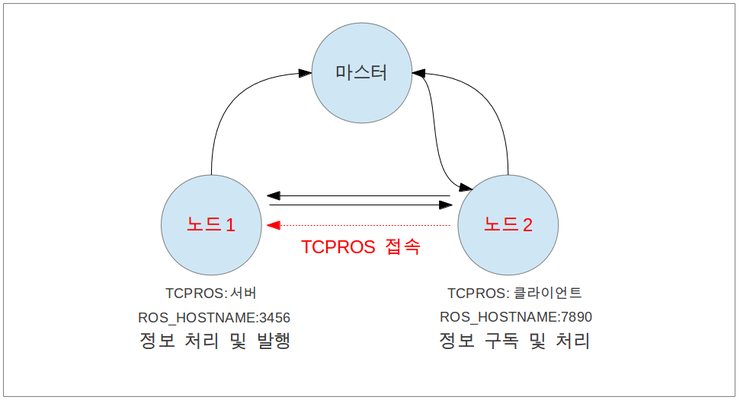
\includegraphics[width=0.9\columnwidth]{pictures/chapter4/notion7.png}
\caption{TCP 접속}
\end{figure}

%-------------------------------------------------------------------------------
\subsection{메시지 전송}\index{메시지 전송}

발행자 노드는 구독자 노드에게 정해진 메시지를 전송한다. (노드간의 통신 방식으로는 TCPROS라 하는 TCP/IP 방식을 이용한다.)

\begin{figure}[h]
\centering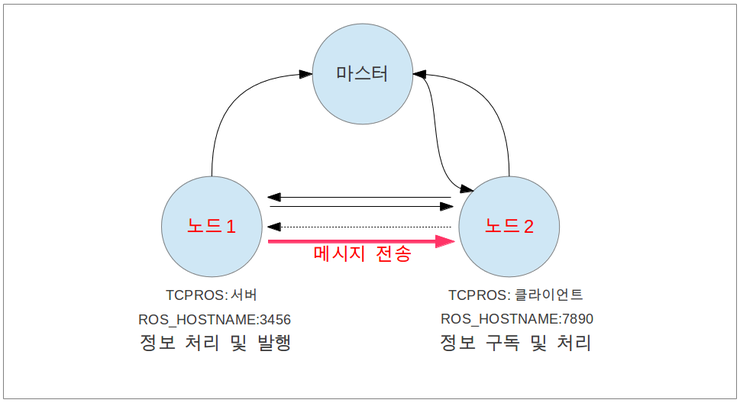
\includegraphics[width=0.9\columnwidth]{pictures/chapter4/notion8.png}
\caption{메시지 전송}
\end{figure}

\newpage
%-------------------------------------------------------------------------------
\subsection{서비스 요청 및 응답}\index{서비스 요청 및 응답}

위에서 설명한 내용은 메시지 통신중에 토픽에 해당된다. 토픽의 경우, 발행자 및 구독자가 중지하지 않는 이상, 메시지가 연속적으로 발행되고 구독하게 된다. 서비스의 경우에는 서비스를 요청하는 서비스 클라이언트와 서비스 요청을 받고 정해진 프로세스를 수행 및 응답하는 서비스 서버로 구분된다. 서비스는 토픽과 달리 1회에 한해 접속, 서비스 요청, 서비스 응답이 수행되고 서로간의 접속을 끊는다. 다시 필요한 경우 접속부터 다시 진행해야 한다. 

\begin{figure}[h]
\centering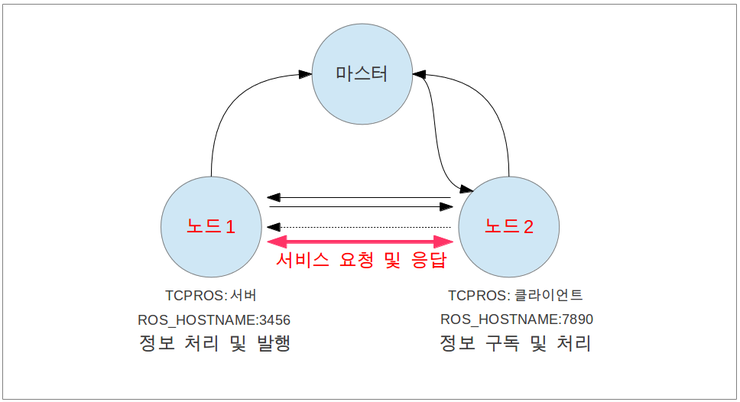
\includegraphics[width=0.7\columnwidth]{pictures/chapter4/notion9.png}
\caption{서비스 요청 및 응답}
\end{figure}

%-------------------------------------------------------------------------------
\subsection{예제}\index{예제}

이전 내용에서 우리는 turtlesim 을 이용하여 ROS의 구동을 테스트 해보았다. 이 테스트에서도 마스터 및 두 개의 노드가 사용되었고, 두 노드간에는 /turtle1/cmd\_vel 이라는 토픽을 이용하여 메시지 통신하고 있다. 이를 위해서 설명한 ROS 개념 맞추어 생각해보면 다음의 그림처럼 생각할 수 있다. 이전 ROS 동작 테스트 내용을 되새김해보며 ROS 개념을 다시 한번 생각해보자.

\begin{figure}[h]
\centering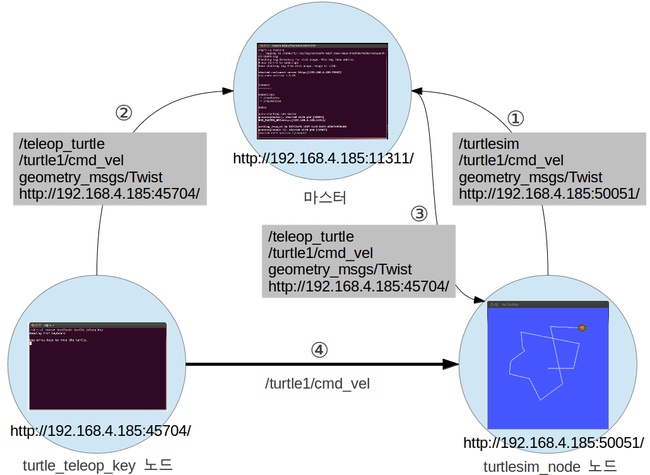
\includegraphics[width=0.8\columnwidth]{pictures/chapter4/notion10.png}
\caption{예제}
\end{figure}

\newpage
%-------------------------------------------------------------------------------
\section{ROS 파일시스템}\index{ROS 파일시스템}

%-------------------------------------------------------------------------------
\subsection{ROS의 파일 시스템}\index{ROS의 파일 시스템}
ROS의 파일 시스템에 대해서 설명하고자 한다. ROS는 ROS 설치 폴더와 사용자 작업 폴더로 구분된다. 
ROS 설치 폴더는 ROS의 데스크톱 버전을 설치하게 되면 /opt 폴더에 /ros 이라는 이름으로 폴더가 생성되고 그 안에 roscore를 포함한 핵심 유틸리티 및 rqt, rviz, 로봇 관련 라이브러리, 시뮬레이션, 네이게이션 등이 설치된다. 사용자는 이 부분의 파일들을 건들일은 거의 없다. 

사용자 작업 폴더는 사용자가 원하는 곳에 폴더를 생성가능한데 필자는 리눅스 사용자 폴더인 \textasciitilde/catkin\_ws/ (\textasciitilde/ 은 리눅스에서 /home/사용자명에 해당되는 폴더를 의미한다.) 에 설치할 것은 추천한다. 

\textbf{챕터~\ref{cha:RosInstall}~\nameref{cha:RosInstall}(pp.\pageref{cha:RosInstall})}에서 설명한 ROS Indigo 설치 및 ROS 개발 환경 구축를 진행했다는 가정하에 ROS 설치 폴더와 사용자 작업 폴더에 대한 상세한 내용을 설명하고자 한다.

%-------------------------------------------------------------------------------
\subsection{ROS 설치 폴더}\index{ROS 설치 폴더}

%-------------------------------------------------------------------------------
\subsubsection{설치 경로}\index{설치 경로}

ROS는 /opt/ros/[버전명] 폴더에 설치된다. 예를 들어, Indigo 버전을 설치하였을 경우 /opt/ros/indigo 가 ROS 설치 경로이다.

%-------------------------------------------------------------------------------
\subsubsection{파일 구성}\index{파일 구성}

다음의 그림과 같이 /opt/ros/indigo 의 폴더 아래에 bin, etc, include, lib, share 폴더 및 몇가지 환경 설정 파일들로 구성되어 있다. 

\begin{figure}[h]
\centering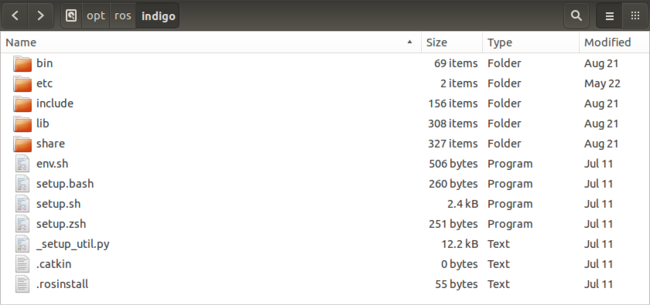
\includegraphics[width=0.7\columnwidth]{pictures/chapter4/folders.png}
\caption{ROS 파일 구성}
\end{figure}

%-------------------------------------------------------------------------------
\subsubsection{세부 내용}\index{세부 내용}
ROS이 폴더에는 ROS 설치시에 선택한 패키지를 포함한 ROS 구동 프로그램을 포함하고 있다. 세부 내용은 아래와 같다.

\begin{itemize}
\item /bin 실행가능한 바이너리 파일
\item /etc ROS 및 catkin 관련 설정파일
\item /include 헤더파일
\item /lib 라이브러리 파일
\item /share ROS 패키지
\item env.* 환경설정 파일
\item setup.* 환경설정 파일
\end{itemize}

%-------------------------------------------------------------------------------
\subsection{사용자 작업 폴더}\index{사용자 작업 폴더}

%-------------------------------------------------------------------------------
\subsubsection{사용자 작업 폴더 경로}\index{사용자 작업 폴더 경로}

사용자 작업 폴더는 사용자가 원하는 곳에 폴더를 생성가능하나 강좌의 원활한 진행을 위하여 리눅스 사용자 폴더인 \textasciitilde/catkin\_ws/ (\textasciitilde/ 은 리눅스에서 /home/사용자명에 해당되는 폴더를 의미한다.) 에 설치할 것은 추천한다. 즉, /home/사용자명/catkin폴더명 으로 설치하면된다. 예를들어 사용자명이 oroca라는 아이디이고 catkin폴더명은 catkin\_ws라고 설정하였다면 /home/oroca/catkin\_ws/ 폴더가 된다.

%-------------------------------------------------------------------------------
\subsubsection{파일 구성}\index{파일 구성}

다음의 그림과 같이 /home/사용자명/ 폴더의 아래에 catkin\_ws 라는 폴더가 있고, build, devel, src 폴더로 구성되어 있다. 

\begin{figure}[h]
\centering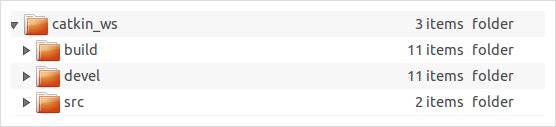
\includegraphics[width=0.65\columnwidth]{pictures/chapter4/folder_catkin_ws.png}
\caption{catkin workspace의 파일 구성}
\end{figure}

%-------------------------------------------------------------------------------
\subsubsection{세부 내용}\index{세부 내용}

이 폴더에는 사용자 작업 폴더로 사용자가 작성한 패키지 및 공개된 다른 개발자의 패키지를 저장하고 빌드하는 공간이다. 사용자는 이 폴더를 작업 폴더로 이용하며 ROS 관련된 내부분의 작업을 이 폴더안에서 하게된다. 세부 내용은 아래와 같다.

\vspace{\baselineskip}
\begin{itemize}[leftmargin=*]
\item /build catkin : 빌드 시스템의 빌드 환경 파일
\item /devel catkin : 빌드 시스템에 의해 빌드된 msg, srv 헤더파일 및 사용자 패키지 라이브러리 및 실행파일
\item /src : 사용자 패키지
\end{itemize}

%-------------------------------------------------------------------------------
\subsubsection{사용자 패키지}\index{사용자 패키지}

\textasciitilde/catkin\_ws/src 폴더에는 사용자가 사용하는 공간이다. 이 폴더에 사용자가 개발한 ROS 패키지 및 다른 개발자가 개발한 패키지를 저장하고 빌드하여 실행 파일을 생성해 낼 수 있다. ROS 빌드 시스템은 다음 강좌를 통해 저 자세히 알아 보도록 하고 이번 강좌에는 "이런 폴더와 파일로 구성되어 있구나" 라고 알아두고 넘어가기로 하자. 아래의 예제는 필자가 작성한 oroca\_ros\_tutorial 이라는 패키지를 작성한 후의 상태이다.

\begin{figure}[h]
\centering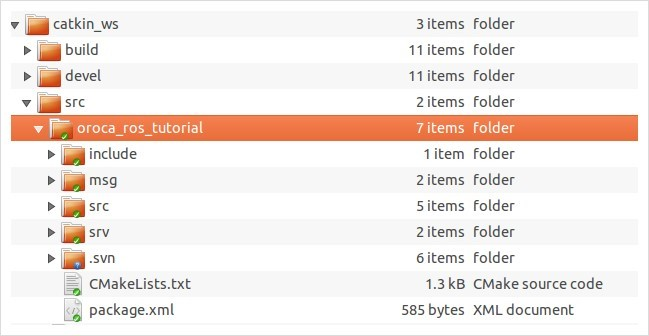
\includegraphics[width=0.65\columnwidth]{pictures/chapter4/folder_oroca_ros_tutorial.jpg}
\caption{사용자 패키지의 파일 구성}
\end{figure}

\begin{itemize}
\item /include 헤더파일
\item /launch ROS런치에 사용되는 스크립트
\item /node rospy용 스크립트
\item /msg 메시지 파일
\item /src 코드 소스 파일
\item /srv 서비스 파일
\item CMakeLists.txt 빌드 설정 파일
\item package.xml 패키지 설정 파일
\end{itemize}

%-------------------------------------------------------------------------------
\section{ROS 빌드 시스템}\index{ROS 빌드 시스템}
\label{sec:RosBuildSystem}

%-------------------------------------------------------------------------------
\subsection{ROS 빌드 시스템}\index{ROS 빌드 시스템}

ROS의 빌드 시스템은 기본적으로 CMake(Cross Platform Make)\footnote{CMake, wikipedia, http://ko.wikipedia.org/wiki/CMake} 를 이용하고 있고, 패키지 폴더에 CMakeLists.txt 라는 파일에 빌드 환경을 기술하고 있다. ROS에서는 CMake를 ROS에 맞도록 수정하여 ROS에 특화된 캐킨 빌드 시스템을 만들었다. 

ROS에서 CMake를 이용하고 있는 이유는 멀티플랫폼에서 ROS 패키지를 빌드할 수 있도록 위함이다. Make\footnote{Make, wikipedia, http://ko.wikipedia.org/wiki/Make}가 유닉스계열만 지원하는 것과 달리, CMake는 유닉스 계열인 리눅스, BSD, OS X 뿐만 아니라 윈도우 계열도 지원하기 때문이다. 또한, 마이크로소프트 비주얼 스튜디오도 지원하고 QT개발에도 쉽게 적용될 수 있다. 

더욱이, 캐킨 빌드 시스템은 ROS와 관련된 빌드, 패키지 관리, 패키지간의 의존관계 등을 편리하게 사용할 수 있도록 하고 있다. 

%-------------------------------------------------------------------------------
\subsection{패키지 생성}\index{패키지 생성}

ROS 패키지를 생성하기 위해서는 다음과 같은 명령어를 이용한다. "catkin\_create\_pkg" 는 사용자가 패키지를 작성할때 캐킨 빌드 시스템에 꼭 필요한 CMakeLists.txt 와 package.xml 를 포함한 패키지 폴더를 생성한다. 실제로 간단한 패키지를 작성해 보자.

\vspace{\baselineskip}
\begin{lstlisting}[language=ROS]
$ catkin_create_pkg %*[패키지이름] [의존하는패키지1] [의존하는패키지2] [의존하는패키지3]*)
\end{lstlisting}

%-------------------------------------------------------------------------------
\subsubsection{작업 폴더로 이동}\index{작업 폴더로 이동}

\vspace{\baselineskip}
\begin{lstlisting}[language=ROS]
$ cd ~/catkin_ws/src
\end{lstlisting}

%-------------------------------------------------------------------------------
\subsubsection{패키지 생성}\index{패키지 생성}

"my\_first\_ros\_pkg" 라는 이름의 패키지를 생성할 것이다. 

ROS에서는 패키지 이름에는 모두 소문자를 사용하며, 스페이스바와 같은 공백이 있으면 안된다. 그리고 일반적으로 하이픈(-) 대신에 밑줄(\_)을 사용하여 각 단어를 이어붙이는 것을 관례로 하고 있다. 

그리고 이번에는 의존하는 패키지로 "std\_msgs"와 "roscpp"를 옵션으로 달아주었다. ROS의 표준 메시지 패키지인 std\_msgs 와 ROS에서 C/C++을 사용하기 위하여 클라이언트라이브러인 roscpp를 사용하겠다는 것으로 패키지 생성에 앞어서 미리 설치해야한다는 의미이다. 이러한 의존하는 패키지의 설정은 패키지 생성할 때 지정할 수도 있지만, 생성 후 package.xml 에서 직접 입력하여도 된다.

\vspace{\baselineskip}
\begin{lstlisting}[language=ROS]
$ catkin_create_pkg my_first_ros_pkg std_msgs roscpp
\end{lstlisting}

위와 같이 패키지를 생성하였으면 "\textasciitilde/catkin\_ws/src"에 "my\_first\_ros\_pkg" 라는 패키지 폴더 및 ROS 패키지가 갖추어야할 기본 내부 폴더 및 CMakeLists.txt 와 package.xml가 생성된다. 다음과 같이 명령어로 ls 를 입력하여 내용을 보던가 윈도우의 탐색기와 같은 역할을 하는 GUI기반의 Nautilus를 이용하여 패키지 내부를 살펴보도록 하자.

\vspace{\baselineskip}
\begin{lstlisting}[language=ROS]
$ ls
include       %*.......... 인클루드 폴더*)
src           %*.......... 소스코드 폴더*)
CMakeLists.txt%*.......... 빌드 설정 파일*)
package.xml   %*.......... 패키지 설정 파일*)
\end{lstlisting}

\begin{figure}[h]
\centering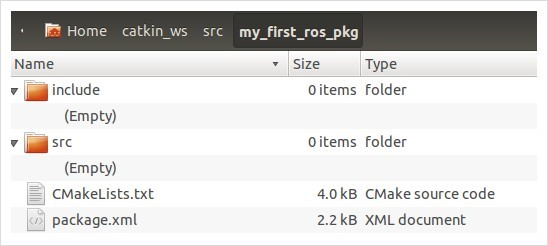
\includegraphics[width=0.6\columnwidth]{pictures/chapter4/new_package.jpg}
\caption{caption}
\end{figure}

%-------------------------------------------------------------------------------
\subsection{패키지 설정 파일 (package.xml) 수정}\index{패키지 설정 파일 (package.xml) 수정}

ROS의 필수 설정 파일 중 하나인 package.xml 은 패키지의 정보를 담은 XML 파일로써 패키지의 이름, 저작자, 라이선스, 의존성 패키지 등을 기술하고 있다. 처음에 아무런 수정을 가하지 않은 원본 파일은 다음과 같다.

\vspace{\baselineskip}
\lstinputlisting[language=XML, numbers=none, caption=package.xml]{./sources/package.xml}

\vspace{\baselineskip}
\begin{itemize}[leftmargin=*]
\item \textless{?xml}\textgreater~문서 분법을 정의하는 문구로 아래의 내용은 xml 버전 1.0을 따르고 있다는 것을 알리고 있다.
\item \textless{package}\textgreater~이 구문부터 \textless/package\textgreater 까지가 ROS 패키지 설정 부분이다.
\item \textless{name}\textgreater~패키지의 이름이다. 패키지 생성할때 입력한 패키지 이름이 사용된다. 다른 옵션도 마찬가지이지만 이는 사용자가 원할때 언제든지 변경할 수 있다.
\item \textless{version}\textgreater~패키지의 버전이다. 자유롭게 지정할 수 있다.
\item \textless{description}\textgreater~패키지의 간단한 설명이다. 
\item \textless{maintainer}\textgreater~패키지 관리자의 연락처를 기재한다.
\item \textless{license}\textgreater~라이선스를 기재한다. BSD, MIT, GPLv3, LGPLv3 등을 기재하면 된다. 오로카에서는 MIT를 사용하고 있다.
\item \textless{url}\textgreater~패키지를 설명하는 웹 페이지 또는 버그관리, 저장소 등의 주소를 기입한다. 이 종류에 따라 type에  website, bugtracker, repository 를 대입하면 된다. 참고로 url 태그는 옵션이다.
\item \textless{author}\textgreater~패키지 개발에 참여한 개발자를 적어주면 된다. 참고로 author 태그는 옵션이다.
\item \textless{buildtool\_depend}\textgreater~빌드 시스템의 의존성을 기술한다. 지금은 캐킨 빌드 시스템을 이용하고 있기 때문에 catkin 를 입력하면 된다.
\item \textless{build\_depend}\textgreater~패키지를 빌드할 때 의존하는 패키지명을 적어준다.
\item \textless{run\_depend}\textgreater~패키지를 실행할 때 의존하는 패키지명을 적어준다.
\item \textless{test\_depend}\textgreater~패키지를 테스트할때 의존하는 패키지명을 적어준다. 테스트이외에는 사용하지 않는다.
\item \textless{export}\textgreater~ROS에서 명시하지 않은 태그명을 사용할때 쓰인다. 일반적인 경우 쓸일이 없다.
\item \textless{metapackage/}\textgreater~export 태그 안에서 사용하는 공식적인 태그로 현재의 패키지가 메타패키지의 경우 이를 선언한다.
\end{itemize}

\vspace{\baselineskip}
\noindent
필자는 다음과 같이 패키지 설정 파일(package.xml)을 수정하였다. 여러분은 자신에 맞게 수정해보도록 하자.

\vspace{\baselineskip}
\begin{lstlisting}[language=XML]
<?xml version="1.0"?>
<package>
  <name>my_first_ros_pkg</name>
  <version>0.0.1</version>
  <description>The my_first_ros_pkg package</description>
 
  <maintainer email="passionvirus@gmail.com">Yoonseok Pyo</maintainer>
  <license>MIT</license>
  <url type="website">http://cafe.naver.com/openrt/2500</url>
  <url type="repository">https://github.com/oroca/oroca_ros_tutorials.git</url>
  <author email="passionvirus@gmail.com">Yoonseok Pyo</author>
 
  <buildtool_depend>catkin</buildtool_depend>
 
  <build_depend>std_msgs</build_depend>
  <build_depend>roscpp</build_depend>
 
  <run_depend>std_msgs</run_depend>
  <run_depend>roscpp</run_depend>
 
  <export>
  </export>
</package>
\end{lstlisting}

%-------------------------------------------------------------------------------
\subsection{빌드 설정 파일 (CMakeLists.txt) 수정}\index{빌드 설정 파일 (CMakeLists.txt) 수정}

ROS의 빌드 시스템인 캐킨은 기본적으로 CMake를 이용하고 있어서 패키지 폴더에 CMakeLists.txt 라는 파일에 빌드 환경을 기술하고 있다. 이는 실행 파일 생성, 의존성 패키지 우선 빌드, 링크 생성 등을 설정하게 되어 있다. 처음에 아무런 수정을 가하지 않은 원본 파일은 다음과 같다.

\lstinputlisting[language=make, numbers=none, caption=CMakeLists.txt]{./sources/CMakeLists.txt}

\noindent
빌드 설정 파일 (CMakeLists.txt)의 각 옵션들은 다음과 같다.\\

운영체제에 설치되어 있는 cmake의 최소한의 버전이다. 현재에는 2.8.3 버전으로 명시되어 있다. 이 보다 낮은 cmake를 사용하는 경우에는 버전 업데이트를 해줘야 한다.
\begin{lstlisting}[language=make]
cmake_minimum_required(VERSION 2.8.3)
\end{lstlisting}

패키지의 이름이다. package.xml 에서 입력한 패키지 이름을 그대로 사용하자.
\begin{lstlisting}[language=make]
project(my_first_ros_pkg)
\end{lstlisting}

캐킨 빌드를 할 때 요구되는 구성요소 패키지이다. 현재 의존성 패키지로 roscpp 및 std\_msgs가 추가되어 있다. 여기에 입력된 패키지가 없는 경우 캐킨 빌드할 때 사용자에게 에러가 표시된다. 즉, 사용자가 만든 패키지가 의존하는 패키지를 먼저 설치하게 만드는 옵션이다.
\begin{lstlisting}[language=make]
find_package(catkin REQUIRED COMPONENTS
  roscpp
  std_msgs
)
\end{lstlisting}

ROS 이외의 패키지를 사용하는 경우에 사용되는 방법이다. 예를들어 다음의 경우, Boost를 사용할때 system 이라는 패키지가 설되어 있어야 한다. 기능은 위에서 설명한 의존하는 패키지를 먼저 설치하게 만드는 옵션이다.
\begin{lstlisting}[language=make]
find_package(Boost REQUIRED COMPONENTS system)
\end{lstlisting}

파이썬을 사용할 때 설정하는 옵션이다. 파이썬은 cmake를 사용할 필요없는 스크립트 언어이지만 패키지의 호환성을 위해 아래와 같이 독자적인 설정을 하게 되어 있다.
\begin{lstlisting}[language=make]
catkin_python_setup()
\end{lstlisting}

사용하는 메시지 파일을 추가하는 옵션이다. FILES를 사용하면 패키지 폴더의 msg 폴더안의 .msg 파일들을 참조하게 된다. 다음의 예제에서는 Message1.msg 및 Message2.msg 의 메시지 파일을 이용하겠다는 옵션이다.
\begin{lstlisting}[language=make]
add_message_files(
  FILES
  Message1.msg
  Message2.msg
)
\end{lstlisting}

사용하는 서비스 파일을 추가하는 옵션이다. FILES를 사용하면 패키지 폴더의 srv 폴더안의 .srv 파일들을 참조하게 된다. 다음의 예제에서는 Service1.srv 및 Service2.srv 의 서비스 파일을 이용하겠다는 옵션이다.
\begin{lstlisting}[language=make]
add_service_files(
  FILES
  Service1.srv
  Service2.srv
)
\end{lstlisting}

의존하는 메시지를 사용하겠다는 옵션이다. 다음의 예제에서는 DEPENDENCIES 옵션에 의하여 std\_msgs 라는 메시지 패키지를 사용하겠다는 설정이다.
\begin{lstlisting}[language=make]
generate_messages(
  DEPENDENCIES
  std_msgs
)
\end{lstlisting}

캐킨 빌드 옵션이다. "INCLUDE\_DIRS"는 뒤에 설정한 패키지 내부 폴더인 "include"의 헤더파일을 사용하겠다는 설정이다. "LIBRARIES"는 뒤에 설정한 패키지의 라이브러리를 사용하겠다는 설정이다. "CATKIN\_DEPENDS" 캐킨 빌드할 때 의존하는 패키지들이다. 현재 roscpp 및 std\_msgs가 의존하고 있다는 설정이다. "DEPENDS" 시스템 의존 패키지를 기술하는 설정이다.
\begin{lstlisting}[language=make]
catkin_package(
 INCLUDE_DIRS include
 LIBRARIES my_first_ros_pkg
 CATKIN_DEPENDS roscpp std_msgs
 DEPENDS system_lib
)
\end{lstlisting}

인클루드 폴더를 지정할 수 있는 옵션이다. 현재 \$\{catkin\_INCLUDE\_DIRS\} 라고 설정되어 있는데 이는 각 패키지안의 "include" 폴더를 의미하고 이 안의 헤더파일을 이용 하겠다는 설정이다.
\begin{lstlisting}[language=make]
include_directories(
  ${catkin_INCLUDE_DIRS}
)
\end{lstlisting}

cpp 라이브러리를 선언한다. src/\$\{PROJECT\_NAME\}/my\_first\_ros\_pkg.cpp 파일을 참조하여 my\_first\_ros\_pkg 라는 라이브러리를 생성하게 된다.
\begin{lstlisting}[language=make]
add_library(my_first_ros_pkg
  src/\${PROJECT_NAME}/my_first_ros_pkg.cpp
)
\end{lstlisting}

cpp 실행 파일을 선언한다. src/my\_first\_ros\_pkg\_node.cpp 파일을 참조하여 my\_first\_ros\_pkg\_node 라는 실행파일을 생성한다.
\begin{lstlisting}[language=make]
add_executable(my_first_ros_pkg_node src/my_first_ros_pkg_node.cpp)
\end{lstlisting}

패키지를 빌드하기 앞서서 생성해야할 메시지 헤더파일이 있을 경우 빌드전에 우선적으로 메시지를 생성하라는 설정이다. 현재 my\_first\_ros\_pkg\_generate\_messages\_cpp 를 우선적으로 빌드하고 my\_first\_ros\_pkg\_node 를 빌드하게 하는 설정이다.
\begin{lstlisting}[language=make]
add_dependencies(my_first_ros_pkg_node my_first_ros_pkg_generate_messages_cpp)
\end{lstlisting}

my\_first\_ros\_pkg\_node 를 생성하기 앞서서 링크해야하는 라이브러리 및 실행파일을 링크해주는 옵션이다.
\begin{lstlisting}[language=make]
target_link_libraries(my_first_ros_pkg_node
  \${catkin_LIBRARIES}
)
\end{lstlisting}

\noindent
필자는 다음과 같이 빌드 설정 파일(CMakelists.txt)을 수정하였다. 여러분은 자신에 맞게 수정해보도록 하자.

\begin{lstlisting}[language=make]
cmake_minimum_required(VERSION 2.8.3)
project(my_first_ros_pkg)
 
find_package(catkin REQUIRED COMPONENTS
  roscpp
  std_msgs
)
 
catkin_package(
  INCLUDE_DIRS include
  CATKIN_DEPENDS roscpp std_msgs
  DEPENDS system_lib
)
 
include_directories( ${catkin_INCLUDE_DIRS} )
 
add_executable(hello_world_node src/hello_world_node.cpp)
add_dependencies(hello_world_node my_first_ros_pkg_generate_messages_cpp)
target_link_libraries(hello_world_node ${catkin_LIBRARIES})
\end{lstlisting}

\newpage
%-------------------------------------------------------------------------------
\subsection{소스코드 작성}\index{소스코드 작성}

\vspace{\baselineskip}
\begin{lstlisting}[language=make]
add\_executable(hello\_world\_node src/hello\_world\_node.cpp)
\end{lstlisting}

위에서 설명한 CMakelists.txt 파일의 실행 파일 생성 부분(add\_executable)에서 위와 같이 설정해 놓았다. 즉, 패키지의 "src" 폴더에 있는 "hello\_world\_node.cpp" 소스 코드를 참고하여 "hello\_world\_node" 라는 실행 파일을 생성하라는 설정이다. 여기서, "hello\_world\_node.cpp" 소스코드가 없기에 간단한 예제로 하나 작성해 보자. 다음의 예제에서는 nano라는 에디터를 사용하였으나 vi, gedit, qtcreator 등 자신이 원하는 편집기를 이용하면 된다.

\vspace{\baselineskip}
\begin{lstlisting}[language=ROS]
$ cd /src     %* //여기서 src 는 자신의 패키지 폴더안의 src 라는 소스코드를 담는 폴더를 말한다.*)
$ nano hello_world_node.cpp
\end{lstlisting}

\begin{lstlisting}[language=C++]
#include <ros/ros.h>
#include <std_msgs/String.h>

#include <sstream>

int main(int argc, char **argv)
{
  ros::init(argc, argv, "hello_world_node");
  ros::NodeHandle nh;
  ros::Publisher chatter_pub = nh.advertise<std_msgs::String>("say_hello_world", 1000);

  ros::Rate loop_rate(10);
  int count = 0;
  while (ros::ok())
  {
    std_msgs::String msg;
    std::stringstream ss;
    ss << "hello world " << count;
    msg.data = ss.str();
    ROS_INFO("%s", msg.data.c_str());
    chatter_pub.publish(msg);
    ros::spinOnce();
    loop_rate.sleep();
    ++count;
  }
  return 0;
}
\end{lstlisting}

%-------------------------------------------------------------------------------
\subsection{패키지 빌드}\index{패키지 빌드}

이제 패키지 빌드를 위한 모든 작업이 완료되었다.  빌드에 앞서서 다음의 명령어로 ROS 패키지의 프로파일을 갱신시켜주자. 앞서 제작한 우리의 패키지를 ROS 패키지 목록에 반영시켜주는 명령어이다. 필수 사항은 아니지만 새로 패키지를 생성한 후에 갱신해주면 이용하기 편하다.

\vspace{\baselineskip}
\begin{lstlisting}[language=ROS]
$ rospack profile
\end{lstlisting}

\noindent
다음은 캐킨 빌드 이다. 캐킨 작업 폴더로 이용하여 캐킨 빌드를 해주자.

\vspace{\baselineskip}
\begin{lstlisting}[language=ROS]
$ cd ~/catkin_ws && catkin_make
%*또는*)
$ cm
\end{lstlisting}

\noindent
이전 강좌인 "ROS 강좌 : 06. ROS 개발 환경 구축"에서 언급했듯이 .bashrc 파일에 alias \verb|cm='cd ~/catkin_ws && catkin_make'| 라고 설정해두면 터미널 창에서 "cm" 이라는 간단한 명령어로 위의 명령어를 대체할 수 있다. 유용한 만큼 이전 강좌를 보고 꼭 설정해 두도록 하자.

%-------------------------------------------------------------------------------
\subsection{노드 실행}\index{노드 실행}

에러 없이 빌드가 완료되었으면 "\textasciitilde/catkin\_ws/devel/lib/my\_first\_ros\_pkg" 에 "hello\_world\_node" 라는 파일이 생성되었을 것이다. 한번 확인해 보자.

다음 단계는 노드를 실행하는 것인데 노드 실행에 앞서서 roscore를 구동하자. ROS의 모든 노드는 roscore를 구동한 후에 이용할 수 있다.

\vspace{\baselineskip}
\begin{lstlisting}[language=ROS]
$ roscore
\end{lstlisting}

\noindent
마지막으로 새로운 터미널창을 열어 아래의 명령어로 노드를 실행해보자. my\_first\_ros\_pkg 라는 패키지의 hello\_world\_node 라는 노드를 실행하라는 명령어이다.

\vspace{\baselineskip}
\begin{lstlisting}[language=ROS]
$ rosrun my_first_ros_pkg hello_world_node 
[ INFO] [1380598894.131775283]: hello world 0
[ INFO] [1380598894.231826916]: hello world 1
[ INFO] [1380598894.331798085]: hello world 2
[ INFO] [1380598894.431796634]: hello world 3
[ INFO] [1380598894.531808660]: hello world 4
[ INFO] [1380598894.631800431]: hello world 5
[ INFO] [1380598894.731805683]: hello world 6
\end{lstlisting}

\noindent
노드를 실행하게 되면 위와 같이 hello world 1, 2 ,3 과 같은 메시지가 발행되는 것을 볼 수 있을 것이다. 이번 강좌는 ROS의 빌드 시스템을 설명하기 위한 것이니 노드의 소스코드에 관해서는 다음 강좌를 통해 알아보도록 하자.


%-------------------------------------------------------------------------------
% -*- root: main.tex -*-

%-------------------------------------------------------------------------------
\chapterimage{chapter_head_5.pdf} 

%-------------------------------------------------------------------------------
\chapter{ROS 명령어}

%-------------------------------------------------------------------------------
\section{ROS 명령어 정리}\index{ROS 명령어 정리}
\label{sec:RosCommand}

ROS는 쉘(shell)환경에서 명령어로 파일 시스템 이용, 소스코드 편집, 빌드, 디버깅, 패키지 관리 등을 처리할 수 있다. ROS를 제대로 사용하기 위해서는 기본적인 리눅스 명령어 이외에도 ROS만의 고유한 명령어\footnote{ROS, CommandLineTools, http://wiki.ros.org/ROS/CommandLineTools}들을 익힐 필요가 있다. ROS 명령어로는 다음과 같이 다양하게 존재한다. 

처음부터 모든 명령어를 숙련하게 사용할 수 없겠지만, 다음의 내용을 보고 필요할 때마다 이용하면 되겠다. 처음에는 익숙하지 않아서 불편하게 느껴질 수 있겠지만, 사용하면 사용할 수록 매우 빠르고 편하게 각종 기능을 명령어로 처리하는 자신의 모습을 보게 될 것이다.

ROS의 다양한 명령어를 숙달하기 위하여 본 강좌에서는 우선 각 명령어의 기능을 간단히 설명하고, 하나 하나 예제를 들어가며 소개하도록 하겠다. 그리고 각 명령어의 사용 빈도 및 중요도를 고려하여 필자가 별표로 점수를 매겨두었다. 별표가 많은 명령어의 경우, 사용 빈도수가 높고 중요한 명령어이니 꼭 익혀두기로 하자.

\vspace{\baselineskip}
\noindent
\textbf{[ROS 쉘 명령어]}
\begin{description}
\item[roscd] (★★★) ros+cd(changes directory) : ROS 패키지 또는 스택의 디렉토리 변경 명령어
\item[rospd] (☆☆☆) ros+pushd : ROS 디렉토리 인덱스에 디렉토리 추가
\item[rosd] (☆☆☆) ros+directory : ROS 디렉토리 인덱스 확인 명령어
\item[rosls] (★☆☆) ros+ls(lists files) : ROS 패키지의 파일 리스트를 확인하는 명령어
\item[rosed] (★☆☆) ros+ed(editor) : ROS 패키지의 파일을 편집하는 명령어
\item[roscp] (☆☆☆) ros+cp(copies files) : ROS 패키지의 파일 복사하는 명령어
\end{description}

\vspace{\baselineskip}
\noindent
\textbf{[ROS 실행 명령어]}
\begin{description}
\item[roscore] (★★★) ros+core : master (ROS 네임 서비스) + rosout (stdout/stderr) + parameter server (매개변수관리)
\item[rosrun] (★★★) ros+run : 패키지의 노드를 실행하는 명령어
\item[roslaunch] (★★★) ros+launch : 패키지의 노드를 복수개 실행하는 명령어
\item[rosclean] (★☆☆) ros+clean : ros 로그 파일을 체크하거나 삭제하는 명령어
\end{description}

\vspace{\baselineskip}
\noindent
\textbf{[ROS 정보 명령어]}
\begin{description}
\item[rostopic] (★★★) ros+topic : ROS 토픽 정보를 확인하는 명령어
\item[rosservice] (★★★) ros+service : ROS 서비스 정보를 확인하는 명령어
\item[rosnode] (★★★) ros+node : ROS의 노드 정보를 얻는 명령어
\item[rosparam] (★★★) ros+param(parameter) : ROS 파라미터 정보를 확인, 수정 가능한 명령어
\item[rosmsg] (★★☆) ros+msg : ROS 메세지 선언 정보를 확인하는 명령어
\item[rossrv] (★★☆) ros+srv : ROS 서비스 선언 정보를 확인하는 명령어
\item[roswtf] (☆☆☆) ros+wtf : ROS 시스템을 검사하는 명령어
\item[rosversion] (★☆☆) ros+version : ros 패키및 배포 릴리즈 버전의 정보를 확인하는 명령어
\item[rosbag] (★★★) ros+bag : ROS 메세지를 기록, 재생하는 명령어
\end{description}

\vspace{\baselineskip}
\noindent
\textbf{[ROS 캐킨 명령어]}
\begin{description}
\item[catkin\_create\_pkg] (★★★) 캐킨 빌드 시스템에 의한 패키지 자동 생성
\item[catkin\_eclipse] (★★☆) 캐킨 빌드 시스템에 의해 생성된 패키지를 이클립스에서 사용할 수 있도록 변경하는 명령어
\item[catkin\_find] (☆☆☆) 캐킨 검색
\item[catkin\_generate\_changelog] (☆☆☆) 캐킨 변경로그 생성
\item[catkin\_init\_workspace] (★☆☆) 캐킨 빌드 시스템의 작업폴더 초기화
\item[catkin\_make] (★★★) 캐킨 빌드 시스템을 기반으로한 빌드 명령어
\end{description}

\vspace{\baselineskip}
\noindent
\textbf{[ROS 패키지 명령어]}
\begin{description}
\item[rosmake] (☆☆☆) ros+make : ROS package 를 빌드한다. (구 ROS 빌드 시스템에서 사용됨)
\item[rosinstall] (★☆☆) ros+install : ROS 추가 패키지 설치 명령어
\item[roslocate] (☆☆☆) ros+locate : ROS 패키지 정보 관련 명령어 
\item[roscreate-pkg] (☆☆☆) ros+create-pkg : ROS 패키지를 자동 생성하는 명령어 (구 ROS 빌드 시스템에서 사용됨)
\item[rosdep] (★☆☆) ros+dep(endencies) : 해당 패키지의 의존성 파일들을 설치하는 명령어
\item[rospack] (★★☆) ros+pack(age) : ROS 패키지와 관련된 정보를 알아보는 명령어
\end{description}

%-------------------------------------------------------------------------------
\section{ROS 쉘 명령어}\index{ROS 쉘 명령어}

ROS 쉘 명령어는 일명 rosbash\footnote{ROS, rosbash, http://wiki.ros.org/rosbash}라고 부른다. 이는 리눅스에서 일반적으로 사용하는 bash 쉘 명령어를 ROS에서 사용하는 방법이다. 주로 ros 라는 접두사에 cd, pd, d, ls, ed, cp, run 등의 접미사를 붙여서 사용하게 된다. 이와 관련된 명령어들을 아래에 소개한다.  

\vspace{\baselineskip}
\noindent
\begin{description}
\item[roscd] (★★★) ros + cd (changes directory) 
\item[rospd] (☆☆☆) ros + pushd 
\item[rosd] (☆☆☆) ros + directory
\item[rosls] (★☆☆) ros + ls (lists files)
\item[rosed] (★☆☆) ros + ed (editor)
\item[roscp] (☆☆☆) ros+cp (copies files)
\item[rosrun] (★★★) ros+run 
\end{description}

\vspace{\baselineskip}
\noindent
이 중, 비교적 자주 사용되는 roscd, rosls, rosed 명령어에 대해서 자세히 알아보자.

\vspace{\baselineskip}
\noindent
※ rosrun 은 rosbash 에 포함되나 의미상 ROS 실행 명령어이기 때문에 여기서 다루도록 한다.

\newpage
%-------------------------------------------------------------------------------
\subsection{roscd : ROS 디렉토리 이동}\index{roscd : ROS 디렉토리 이동}

\setcounter{num}{0}

\stepcounter{num}\circled{\thenum} 사용법
\begin{lstlisting}[language=ROS]
roscd [%*패키지이름*)]
\end{lstlisting}

\noindent
\stepcounter{num}\circled{\thenum} 사용예
\begin{lstlisting}[language=ROS]
$ roscd turtlesim
\end{lstlisting}

\noindent
\stepcounter{num}\circled{\thenum} 결과값
\begin{lstlisting}[language=ROS]
/opt/ros/indigo/share/turtlesim$
\end{lstlisting}

\noindent
사용예에서 처럼, turtlesim 이라는 패키지 이름을 매개변수로 넣어주고 실행하게 되면 지정된 패키지가 저장된 폴더로 이동하게 된다. 현재 결과에서는 turtlesim 이라는 패키지가 ROS가 설치되어 있는 폴더에 있으므로 위와 같이 나왔으나, 자신이 작성한 패키지의 이름을 매개변수로 넣어주면 자신이 설정한 패키지의 디렉토리로 이동할 수도 있다. 명령어 기반의 ROS를 사용하는데 있어서 매우 사용빈도가 높은 명령어이다.

\vspace{\baselineskip}
\noindent
※ 위와 같은 실행 및 결과를 위해서는 관련 패키지인 ros-indigo-turtlesim 패키지가 설치되어 있어야 한다. 만약 설치되어 있지 않은 경우 설치하도록 하자. 설치 명령어는 sudo apt-get install ros-indigo-turtlesim  이다.

%-------------------------------------------------------------------------------
\subsection{rosls : ROS 리스트 파일}\index{rosls : ROS 리스트 파일}

\setcounter{num}{0}

\stepcounter{num}\circled{\thenum} 사용법
\begin{lstlisting}[language=ROS]
rosls [%*패키지이름*)]
\end{lstlisting}

\noindent
\stepcounter{num}\circled{\thenum} 사용예
\begin{lstlisting}[language=ROS]
$ rosls turtlesim
\end{lstlisting}

\noindent
\stepcounter{num}\circled{\thenum} 결과값
\begin{lstlisting}[language=ROS]
$ rosls turtlesim/
cmake  images  msg  package.xml  srv
\end{lstlisting}

\noindent
지정한 ROS 패키지의 파일 리스트를 확인하는 명령어이다. roscd 명령어를 이용하여 해당 패키지로 이동후에 일반 ls 명령어로 같은 기능을 수행할 수도 있지만, 간혹 바로 확인할 필요가 있을경우에 사용된다. 사용 빈도수는 매우 떨어진다.

%-------------------------------------------------------------------------------
\subsection{rosed : ROS 편집 명령어}\index{rosed : ROS 편집 명령어}

\setcounter{num}{0}

\stepcounter{num}\circled{\thenum} 사용법
\begin{lstlisting}[language=ROS]
rosed [%*패키지이름*)] [%*파일이름*)]
\end{lstlisting}

\noindent
\stepcounter{num}\circled{\thenum} 사용예
\begin{lstlisting}[language=ROS]
$ rosed turtlesim package.xml 
\end{lstlisting}

\noindent
turtlesim 패키지의 package.xml 를 편집하고자 할때 사용하는 명령어이다. 이를 실행하면 사용자가 설정한 에디터로 해당 파일을 열게된다. 급하게 간단히 파일을 수정하고자 할때 사용된다. 사용되는 에디터는 "~/.bashrc" 파일에 export EDITOR='emacs -nw' 와 같이 지정하여 사용가능하다. 필자는 비교적 단순한 편집일 경우 이를 사용한다. 프로그램 작성과 같은 작업 rosed 이외에 자신만의 개발환경을 사용하기를 추천한다.

\vspace{\baselineskip}
\noindent
\stepcounter{num}\circled{\thenum} 결과값
\begin{lstlisting}[language=ROS]
%*사용자가 지정해둔 에디터를 이용하여 해당 파일을 열게된다.*)
\end{lstlisting}

\noindent
바로 명령어창에서 수정이 필요한 단순한 작업에서 많이 사용되지만, 그 이외의 프로그램 작업등에는 비추천이다. 전체적인 사용 빈도수는 매우 떨어진다.

%-------------------------------------------------------------------------------
\section{ROS 실행 명령어}\index{ROS 실행 명령어}

ROS 실행 명령어\footnote{http://wiki.ros.org/rosbash}는 ROS 노드의 실행을 주관한다. 무엇보다 필수는 roscore로 노드간의 네임 서버로 사용된다. 그리고 실행명령어로는 rosrun 및 roslaunch가 있다. rosrun 는 하나의 노드를 실행하게 되며, roslaunch 는 하나이상의 노드를 실행할때 사용된다. 그리고 rosclean 는 노드 실행시 기록되는 로그의 삭제에 사용되는 명령어이다.

\vspace{\baselineskip}
\noindent
\begin{description}
\item[roscore] (★★★) ros+core : master (ROS 네임 서비스) + rosout (stdout/stderr) + parameter server (매개변수관리)
\item[rosrun] (★★★) ros+run : 패키지의 노드를 실행하는 명령어
\item[roslaunch] (★★★) ros+launch : 패키지의 노드를 복수개 실행하는 명령어
\item[rosclean] (★☆☆) ros+clean : ros 로그 파일을 체크하거나 삭제하는 명령어
\end{description}

\newpage
%-------------------------------------------------------------------------------
\subsection{roscore : ROS 코어 실행}\index{roscore : ROS 코어 실행}
\label{subsec:Roscore}

ROS코어\footnote{http://wiki.ros.org/roscore}는 노드들간의 메시지 통신에서 연결 정보를 관리하는 마스터로서, ROS를 사용하기 위해서 제일 먼저 구동해야하는 필수 요소이다. 다음과 같이 "roscore"라는 실행 명령어로 ROS 마스터는 구동되며, XMLRPC으로 서버를 구동하게 된다. 마스터는 노드간의 접속을 위하여 노드들의 이름, 토픽 및 서비스의 이름, 메시지 형태, URI 주소 및 포트를  등록받고, 요청이 있을 경우 이 정보를 다른 노드에게 알려주는 역할을 한다. 

\setcounter{num}{0}

\vspace{\baselineskip}
\noindent
\stepcounter{num}\circled{\thenum} 사용법
\begin{lstlisting}[language=ROS]
roscore [%*옵션*)]
\end{lstlisting}

\noindent
\stepcounter{num}\circled{\thenum} 사용예
\begin{lstlisting}[language=ROS]
$ roscore
\end{lstlisting}

\noindent
위의 명령어로 ROS 코어를 실행하게되면 사용자가 설정해둔 ROS\_MASTER\_URI 를 마스터 URI로 하여, 마스터를 기동하게 된다. ROS\_MASTER\_URI 은 "~/.bashrc" 에서 사용자가 설정하도록 되어있다.

\vspace{\baselineskip}
\noindent
\stepcounter{num}\circled{\thenum} 결과값
\begin{lstlisting}[language=ROS]
$ roscore
... logging to /home/rts/.ros/log/fefe3f-63dc-fege-a5a1-f3r3df3e44/roslaunch-rts-3547.log
Checking log directory for disk usage. This may take awhile.
Press Ctrl-C to interrupt
Done checking log file disk usage. Usage is <1GB.
started roslaunch server http://192.168.4.100:57385/
ros_comm version 1.11.9

SUMMARY
========
PARAMETERS
 * /rosdistro: indigo
 * /rosversion: 1.11.9

NODES

auto-starting new master
process[master]: started with pid [3560]
ROS_MASTER_URI=http://192.168.4.100:11311/

setting /run_id to fefe3f-63dc-fege-a5a1-f3r3df3e44
process[rosout-1]: started with pid [3575]
started core service [/rosout]
\end{lstlisting}

\noindent
위 결과에서 /home/rt/.ros/log/ 폴더에 로그들이 저장되고 있다는 것과 "Ctrl-C" 키로 ROS 코어를 종료할 수 있다느 것, roslaunch server, ROS\_MASTER\_URI 등의 정보, /rosdistro 및 /rosversion의 파라미터 서버, /rosout 의 서비스, /rosout 노드가 실행되었음을 알수 있다.


%-------------------------------------------------------------------------------
\subsection{rosrun : ROS 노드 실행}\index{rosrun : ROS 노드 실행}

rosrun\footnote{http://wiki.ros.org/rosbash}은 지정한 패키지의 하나의 노드를 실행하는 명령어이다. turtlesim 이라는 패키지의 turtlesim\_node 이라는 노드를 실행하는 명령어이다. rosrun은 지정한 패키지의 하나의 노드를 실행시킨다. 

\setcounter{num}{0}

\vspace{\baselineskip}
\noindent
\stepcounter{num}\circled{\thenum} 사용법
\begin{lstlisting}[language=ROS]
rosrun [%*패키지이름*)] [%*노드이름*)]
\end{lstlisting}

\noindent
\stepcounter{num}\circled{\thenum} 사용예
\begin{lstlisting}[language=ROS]
$ rosrun turtlesim turtlesim_node 
\end{lstlisting}

\noindent
\stepcounter{num}\circled{\thenum} 결과값
\begin{lstlisting}[language=ROS]
$ rosrun turtlesim turtlesim_node 
[INFO] [1383445615.677782380]: Starting turtlesim with node name /turtlesim
[INFO] [1383445615.686475328]: Spawning turtle [turtle1] at x=[5.544445], y=[5.544445], theta=[0.000000]
\end{lstlisting}

\begin{figure}[h]
\centering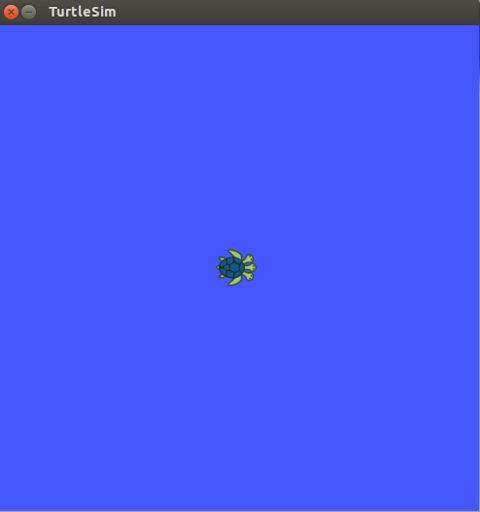
\includegraphics[width=0.7\columnwidth]{pictures/chapter5/term_rosrun.png}
\caption{turtlesim\_node 노드를 실행한 모습}
\end{figure}

\newpage
%-------------------------------------------------------------------------------
\subsection{roslaunch : ROS 노드 복수 실행}\index{roslaunch : ROS 노드 복수 실행}

roslaunch\footnote{http://wiki.ros.org/roslaunch} 지정한 패키지의 하나이상의 노드를 실행하는 명령어이다. 아래와 같이 openni\_launch를 구동하는 것만으로도 camera\_nodelet\_manager, depth\_metric, depth\_metric\_rect, depth\_points 등의 20개 이상의 노드 및 10여개의 파라미터 서버가 실행된다. 이렇듯 런치파일을 이용한 실행은 하나의 패키지의 다수의 노드를 실행하는데 매우 유용하며, ROS에서는 매우 많이 사용되는 실행 방법이다. 이때 사용되는 .launch 파일 작성에 대해서는 \textbf{섹션~\ref{sec:HowToUseTheRoslaunch}~\nameref{sec:HowToUseTheRoslaunch}(pp.\pageref{sec:HowToUseTheRoslaunch})}에서 더 자세히 다루기로 하자.

\setcounter{num}{0}

\vspace{\baselineskip}
\noindent
\stepcounter{num}\circled{\thenum} 사용법
\begin{lstlisting}[language=ROS]
roslaunch [%*패키지이름*)] [%*런치파일명*)]
\end{lstlisting}

\noindent
\stepcounter{num}\circled{\thenum} 사용예
\begin{lstlisting}[language=ROS]
$ roslaunch openni_launch openni.launch 
\end{lstlisting}

\noindent
\stepcounter{num}\circled{\thenum} 결과값
\begin{lstlisting}[language=ROS]
%*생략*)
\end{lstlisting}

\noindent
※ 위와 같은 실행 및 결과를 위해서는 관련 패키지인 ros-indigo-openni-launch 패키지가 설치되어 있어야 한다. 만약 설치되어 있지 않은 경우 설치하도록 하자. 설치 명령어는 sudo apt-get install ros-indigo-openni-launch  이다.

\newpage
%-------------------------------------------------------------------------------
\subsection{rosclean : ROS 로그 파일 삭제}\index{rosclean : ROS 로그 파일 삭제}

ROS 로그 파일을 체크하거나 삭제하는 명령어이다. ROS 코어(roscore)기동과 함께 모든 노드에 대한 기록은 로그파일로 기록되게 되는데 시간이 지날수록 데이타가 축척되므로 주기적으로 rosclean 명령어를 이용하여 삭제할 필요가 있다.

특히, ROS코어 실행시, "WARNING: disk usage in log directory [/xxx/.ros/log] is over 1GB." 이라는 메시지가 표시되면 로그 파일이 1기가를 초과했다는 것이므로 시스템에 무리가 예상이 된다면 rosclean 명령어를 이용하여 삭제하도록 하자.

\setcounter{num}{0}

\vspace{\baselineskip}
\noindent
\stepcounter{num}\circled{\thenum} 사용법
\begin{lstlisting}[language=ROS]
rosclean [%*옵션*)]
\end{lstlisting}

\noindent
\stepcounter{num}\circled{\thenum} 사용예 (rosclean check : 로그 사용 용량 체크)
\begin{lstlisting}[language=ROS]
$ roslaunch openni_launch openni.launch 
\end{lstlisting}

\noindent
\stepcounter{num}\circled{\thenum} 결과값 (rosclean check : 로그 사용 용량 체크)
\begin{lstlisting}[language=ROS]
$ rosclean check
320K ROS node logs
\end{lstlisting}

\noindent
ROS 노드 로그 총 사용량이 320킬로바이트 라는 의미이다.

\vspace{\baselineskip}
\noindent
\stepcounter{num}\circled{\thenum} 사용예 (rosclean purge : 로그 삭제)
\begin{lstlisting}[language=ROS]
$ rosclean purge
\end{lstlisting}

\noindent
\stepcounter{num}\circled{\thenum} 결과값 (rosclean purge : 로그 삭제)
\begin{lstlisting}[language=ROS]
$ rosclean purge 
Purging ROS node logs.
PLEASE BE CAREFUL TO VERIFY THE COMMAND BELOW!
Okay to execute:
rm -rf /home/rt/.ros/log
(y/n)? y
\end{lstlisting}

\noindent
자신의 ROS 로그 저장소 (필자의 경우, /home/rt/.ros/log)의 로그를 모두 삭제할때 사용하는 명령어이다.

\newpage
%-------------------------------------------------------------------------------
\section{ROS 정보 명령어}\index{ROS 정보 명령어}

ROS 정보 명령어는 토픽, 서비스, 노드, 매개변수 등의 정보를 확인하는데 사용되는 명령어로 매우 빈번히 사용되는 명령어군이다. 특히, rostopic, rosservice, rosnode, rosparam는 매우 빈번히 사용되며, rosbag 는 ROS의 큰 특징중에 하나인 데이터 기록, 재생 기능을 갖춘 명령어이므로 꼭 알아두고 활용하도록 하자.

\vspace{\baselineskip}
\noindent
\begin{description}
\item[rosnode] (★★★) ros+node : ROS 노드 관련 명령어
\item[rostopic] (★★★) ros+topic : ROS 토픽 관련 명령어
\item[rosservice] (★★★) ros+service : ROS 서비스 관련 명령어
\item[rosparam] (★★★) ros+param(parameter) : ROS 파라미터 정보를 확인, 수정 가능한 명령어
\item[rosmsg] (★★☆) ros+msg : ROS 메세지 선언 정보를 확인하는 명령어
\item[rossrv] (★★☆) ros+srv : ROS 서비스 선언 정보를 확인하는 명령어
\item[roswtf] (★☆☆) ros+wtf : ROS 시스템을 검사하는 명령어
\item[rosversion] (★☆☆) ros+version : ros 패키및 배포 릴리즈 버전의 정보를 확인하는 명령어
\item[rosbag] (★★★) ros+bag : ROS 메세지를 기록, 재생하는 명령어
\end{description}

%-------------------------------------------------------------------------------
\subsection{노드 실행}\index{노드 실행}

아래의 각 명령어를 사용하기 위해서, ROS에서 제공하는 "turtlesim" 를 이용하여 "turtlesim" 의 관련 노드, 토픽, 서비스 등을 알아 볼 것이다. ROS 정보 명령어를 이용한 테스트를 하기전에 아래처럼 "turtlesim" 관련 노드들을 미리 실행하도록 하자.

%-------------------------------------------------------------------------------
\subsubsection{roscore 실행}

원할한 따라하기식 강좌를 위해 실행 전에 기존에 실행중인 모든 터미널을 닫고 시작해 주길 바란다. 그런다음, 새로운 터미널을 열어 아래와 같은 명렁어를 실행한다. 그러면 아래와 같은 메시지를 보게 되며, 모든 노드를 관할하는 ROS코어가 실행되게 된다.

\begin{lstlisting}[language=ROS]
$ roscore
\end{lstlisting}

%-------------------------------------------------------------------------------
\subsubsection{turtlesim 패키지의 turtlesim\_node 노드 실행}

좀 전과는 다른 새로운 터미널을 열어 아래와 같은 명렁어를 실행한다. 그러면 turtlesim 패키지의 turtlesim\_node를 실행하게 된다. 그러면 파란색 바탕의 화면에 거북이 한마리가 보일 것이다.

\begin{lstlisting}[language=ROS]
$ rosrun turtlesim turtlesim_node 
\end{lstlisting}

%-------------------------------------------------------------------------------
\subsubsection{turtlesim 패키지의 turtle\_teleop\_key 노드 실행}

새로운 터미널을 열어 아래와 같은 명렁어를 실행한다. 그러면 turtlesim 패키지의 turtle\_teleop\_key를 실행하게 된다. 실행된 후, 이 터미널 창의 위에서 키보드의 화살표를 이용하여 거북이를 제어하게 된다. 간단하므로 직접 해보길 바란다. 제어하게 되면 화면 속의 거북이가 움직이게 되는데, 이는 간단히 시뮬레이션이지만 실제 로봇도 이와 같은 방법으로 원격조정이 가능하게 된다.

\begin{lstlisting}[language=ROS]
$ rosrun turtlesim turtle_teleop_key
\end{lstlisting}

\newpage
%-------------------------------------------------------------------------------
\subsection{rosnode : ROS 노드}\index{rosnode : ROS 노드}

우선, 노드(node)에 대해서 이해하고 있어야 한다. 아래 용어정리를 참고하도록 하자. 더 자세한 내용은 섹션~\nameref{sec:RosTerm}(pp.\pageref{def:RosNode})에서 설명해두었다. 참고하도록 하자.

\vspace{\baselineskip}
\noindent
\begin{description}
\item[rosnode list] : 활성화된 노드의 목록 확인
\item[rosnode ping 노드이름] : 지정된 노드와의 연결 테스트
\item[rosnode info 노드이름] : 지정된 노드의 정보 확인
\item[rosnode machine PC이름 또는 IP] : 해당 PC에서 실행되고 있는 노드 목록 확인
\item[rosnode kill 노드이름] : 지정된 노드 실행 중단
\item[rosnode cleanup] : 연결 정보가 확인 안 되는 유령 노드의 등록 정보 삭제
\end{description}

\setcounter{num}{0}

\vspace{\baselineskip}
\noindent
\stepcounter{num}\circled{\thenum} rosnode list : 활성화된 노드의 목록 확인
\begin{lstlisting}[language=ROS]
$ rosnode list
/rosout
/teleop_turtle
/turtlesim
\end{lstlisting}

\noindent
ROS코어(roscore)에 연결된 모든 노드의 목록을 확인하는 명령어이다. 위 [사전준비] 에서 이야기한 노드만을 실행하였다면 위와 같이 roscore를 구동하면 기본적으로 시작되는 rosout 과 [사전준비]에서 실행한 /teleop\_turtle 및 /turtlesim 의 노드가 리스트에 포함되어 있음을 확인할 수 있다.

\vspace{\baselineskip}
\noindent
\stepcounter{num}\circled{\thenum} rosnode ping [노드이름] : 지정된 노드와의 연결 테스트
\begin{lstlisting}[language=ROS]
$ rosnode ping /turtlesim
rosnode: node is [/turtlesim]
pinging /turtlesim with a timeout of 3.0s
xmlrpc reply from http://192.168.4.185:45470/ time=0.854969ms
\end{lstlisting}

\noindent
위 명령어는 /turtlesim 노드가 실제로 현재 사용중인 컴퓨터와 연결이 되어 있는지에 대한 테스트이다. 만약에 해당 노드와 연결되어 있지 않으면 "ERROR: connection refused to [http://192.168.4.185:55996/]" 와 같은 에러 메세지를 보게될 것이다.

\vspace{\baselineskip}
\noindent
\stepcounter{num}\circled{\thenum} rosnode info [노드이름] : 지정된 노드의 정보 확인
\begin{lstlisting}[language=ROS]
$ rosnode info /turtlesim 
-------------------------------
Node [/turtlesim]
Publications: 
 * /turtle1/color_sensor [turtlesim/Color]
...
\end{lstlisting}

\vspace{\baselineskip}
\noindent
rosnode info 명령어를 이용하면 지정한 노드의 정보를 확인가능하다. 기본적으로, Publications, Subscriptions, Services 등을 확인할 수 있으며, 노드 실행 URI 및 토픽 입출력에 대한 정보들도 확인 가능하다. 많은 정보 출력으로 위에서는 내용을 생략해 두었으므 꼭 실행해보길 권장한다.

\noindent
\stepcounter{num}\circled{\thenum} rosnode machine [PC이름 또는 IP] : 해당 PC에서 실행되고 있는 노드 목록 확인
\begin{lstlisting}[language=ROS]
$ rosnode machine 192.168.4.185
/rosout
/teleop_turtle
/turtlesim
\end{lstlisting}

\noindent
지정된 특정 머신(PC 및 단말기)에서 작동죽인 노드의 목록을 확인할 수 있다.

\vspace{\baselineskip}
\noindent
\stepcounter{num}\circled{\thenum} rosnode kill [노드이름] : 지정된 노드 실행 종료
\begin{lstlisting}[language=ROS]
$ rosnode kill /turtlesim
killing /turtlesim
killed
\end{lstlisting}

\noindent
실행중인 노드를 종료하는 명령어이다. 노드가 실행된 터미널창에서 Ctrl + C 를 이용하여 직접 노드를 종료할 수도 있지만, 이렇게 해당 노드를 지정하여 종료할 수도 있다. 만약 이 명령어로 종료하게 되면 아래와 같이 해당 노드가 실행중인 터미널에 경고 메시지가 출력되면서 해당 노드는 종료되게 된다.

\vspace{\baselineskip}
\begin{lstlisting}[language=ROS]
[ WARN] [1383455647.514022654]: Shutdown request received.
[ WARN] [1383455647.514058274]: Reason given for shutdown: [user request]
\end{lstlisting}

\noindent
\stepcounter{num}\circled{\thenum} rosnode cleanup : 연결 정보가 확인안되는 유령 노드의 등록 정보 삭제
\begin{lstlisting}[language=ROS]
$ rosnode cleanup 
\end{lstlisting}

\noindent
연결 정보가 확인안되는 유령 노드의 등록 정보를 삭제한다. 예기치못한 일로 노드가 비정상적으로 종료된경우, 이 명령어로 연결 정보가 끓어진 노드를 목록에서 삭제하게된다. 간혹 사용되지만 roscore 을 재실행하는 일이 없기에 매우 유용한 명령어이다.

\newpage
%-------------------------------------------------------------------------------
\subsection{rostopic : ROS 토픽}\index{rostopic : ROS 토픽}

우선, 토픽(topic)에 대해서 이해하고 있어야 한다. 아래 용어정리를 참고하도록 하자. 더 자세한 내용은 섹션~\nameref{sec:RosTerm}(pp.\pageref{def:RosTopic})에서 설명해두었다. 참고하도록 하자.

\vspace{\baselineskip}
\noindent
\begin{description}
\item[rostopic list] : 활성화된 토픽의 목록을 표시한다
\item[rostopic echo 토픽이름] : 지정한 토픽의 메시지 내용을 실시간으로 표시한다
\item[rostopic find 타입이름] : 지정한 타입의 메시지를 사용하는 토픽을 표시한다
\item[rostopic type 토픽이름] : 지정한 토픽의 메시지 타입을 표시한다
\item[rostopic bw 토픽이름] : 지정한 토픽의 메시지 데이터 대역폭(bandwidth)을 표시한다
\item[rostopic hz 토픽이름] : 지정한 토픽의 메세지 데이터 발행주기를 표시한다
\item[rostopic info 토픽이름] : 지정한 토픽의 정보를 표시한다
\item[rostopic pub 토픽이름 메시지타입 매개변수] : 지정한 토픽의 이름으로 메시지를 발행한다
\end{description}

\vspace{\baselineskip}
\noindent
※ 아래의 예제를 실행하기 전에 모든 노드를 종료하도록 하자. 그리고 난후, 각각 다른 터미널창에서 아래의 명령어를 실행하여 turtlesim\_node 및 turtle\_teleop\_key를 실행해주자.

\begin{lstlisting}[language=ROS]
roscore
rosrun turtlesim turtlesim_node 
rosrun turtlesim turtle_teleop_key
\end{lstlisting}

\setcounter{num}{0}

\noindent
\stepcounter{num}\circled{\thenum} rostopic list : 활성화된 토픽의 목록을 표시한다

\begin{lstlisting}[language=ROS]
$ rostopic list
/rosout
/rosout_agg
/turtle1/cmd_vel
/turtle1/color_sensor
/turtle1/pose
\end{lstlisting}

\noindent
rostopic list 명령어는 현재 송신 및 수신되고 있는 모든 토픽의 리스트를 확인할 수 있게 해준다.

\begin{lstlisting}[language=ROS]
$ rostopic list -v

Published topics:
 * /turtle1/color_sensor [turtlesim/Color] 1 publisher
 * /turtle1/cmd_vel [geometry_msgs/Twist] 1 publisher
 * /rosout [rosgraph_msgs/Log] 2 publishers
 * /rosout_agg [rosgraph_msgs/Log] 1 publisher
 * /turtle1/pose [turtlesim/Pose] 1 publisher

Subscribed topics:
 * /turtle1/cmd_vel [geometry_msgs/Twist] 1 subscriber
 * /rosout [rosgraph_msgs/Log] 1 subscriber
\end{lstlisting}

\noindent
rostopic list 명령어에 -v 이라는 옵션을 추가해주면, 발행되고 있는 토픽 및 수신되고 있는 토픽을 나누어 주고, 각 토픽의 메시지 타입까지 함께 표시해준다.

\vspace{\baselineskip}
\noindent
\stepcounter{num}\circled{\thenum} rostopic echo [토픽이름] : 지정한 토픽의 메시지 내용을 실시간으로 표시한다.

\begin{lstlisting}[language=ROS]
$ rostopic echo /turtle1/pose 
x: 5.35244464874
y: 5.544444561
theta: 0.0
linear_velocity: 0.0
angular_velocity: 0.0
---
...
\end{lstlisting}

\noindent
/turtle1/pose 토픽을 구성하는 x, y, theta, linear\_velocity, angular\_velocity 의 데이터를 실시간으로 확인할 수 있다.

\vspace{\baselineskip}
\noindent
\stepcounter{num}\circled{\thenum} rostopic find [타입이름] : 지정한 타입의 메시지를 사용하는 토픽을 표시한다

\begin{lstlisting}[language=ROS]
$ rostopic find turtlesim/Pose
/turtle1/pose
\end{lstlisting}

\vspace{\baselineskip}
\noindent
\stepcounter{num}\circled{\thenum} rostopic type [토픽이름] : 지정한 토픽의 메시지 타입을 표시한다

\begin{lstlisting}[language=ROS]
$ rostopic type /turtle1/pose 
turtlesim/Pose
\end{lstlisting}

\vspace{\baselineskip}
\noindent
\stepcounter{num}\circled{\thenum} rostopic bw [토픽이름] : 지정한 토픽의 메시지 데이터 대역폭(bandwidth)을 표시한다

\begin{lstlisting}[language=ROS]
$ rostopic bw /turtle1/pose 
subscribed to [/turtle1/pose]
average: 1.27KB/s
 mean: 0.02KB min: 0.02KB max: 0.02KB window: 62
...
\end{lstlisting}

\noindent
/turtle1/pose 토픽에 사용되는 데이터 대역폭은 초당 1.27KB 임을 확인할 수 있다.

\vspace{\baselineskip}
\noindent
\stepcounter{num}\circled{\thenum} rostopic hz [토픽이름] : 지정한 토픽의 메세지 데이터 발행주기를 표시한다

\begin{lstlisting}[language=ROS]
$ rostopic hz /turtle1/pose 
subscribed to [/turtle1/pose]
average rate: 62.502
 min: 0.016s max: 0.016s std dev: 0.00005s window: 62
\end{lstlisting}

\noindent
/turtle1/pose 의 데이타의 발행 주기를 확인해 볼 수 있다. 위의 결과로는 약 62.5Hz (0.016초=16msec) 주기로 메시지가 발행되고 있음을 알 수 있다.

\vspace{\baselineskip}
\noindent
\stepcounter{num}\circled{\thenum} rostopic info [토픽이름] : 지정한 토픽의 정보를 표시한다

\begin{lstlisting}[language=ROS]
$ rostopic info /turtle1/pose 
Type: turtlesim/Pose
Publishers: 
 * /turtlesim (http://192.168.4.185:42443/)
Subscribers: None
\end{lstlisting}

\noindent
/turtle1/pose 토픽은 turtlesim/Pose 메시지 타입을 사용하고 있고, /turtlesim 노드에 발행되고 있으며, 구독되고 있는 토픽은 없다는 정보를 확인할 수 있다. 

\vspace{\baselineskip}
\noindent
\stepcounter{num}\circled{\thenum} rostopic pub [토픽이름] [메시지타입] [매개변수] : 지정한 토픽의 이름으로 메시지를 발행한다

\begin{lstlisting}[language=ROS]
$ rostopic pub -1 /turtle1/cmd_vel geometry_msgs/Twist -- '[2.0, 0.0, 0.0]' '[0.0, 0.0, 1.8]'
publishing and latching message for 3.0 seconds
\end{lstlisting}

\noindent
/turtle1/pose 토픽은 turtlesim/Pose 메시지 타입을 사용하고 있고, /turtlesim 노드에 발행되고 있으며, 구독되고 있는 토픽은 없다는 정보를 확인할 수 있다. 

\vspace{\baselineskip}
\noindent
\textbf{[옵션 값 지정에 대한 설명]}
\begin{itemize}[leftmargin=*]
\item \textbf{-1} : 메시지를 1번만 발행한다. (실제로는 1번 실행이기는 하지만 위의 결과처럼 3초간 실행된다.)
\item \textbf{/turtle1/cmd\_vel} : 지정한 토픽이름
\item \textbf{geometry\_msgs/Twist} : 발행되는 메시지 타입 이름
\item \textbf{-- '[2.0, 0.0, 0.0]' '[0.0, 0.0, 1.8]'} : x축 좌표로 초당 2.0 미터(m/s)의 속도 이동, z축 좌표로 초당 1.8 라디안 (radian/s) 회전을 하라는 값이다.
\end{itemize}

\begin{figure}[h]
\centering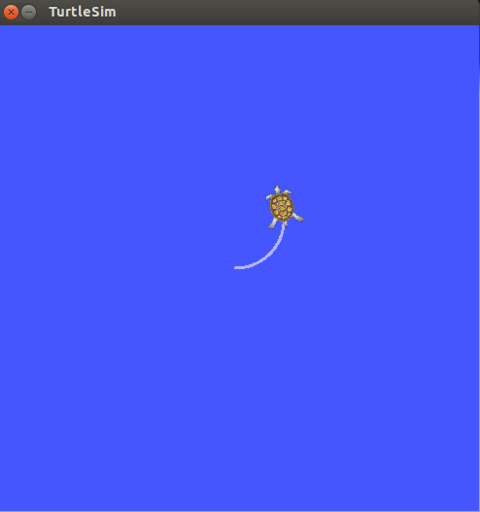
\includegraphics[width=0.7\columnwidth]{pictures/chapter5/rostopic_pub.png}
\caption{발행된 메시지가 반영된 모습}
\end{figure}

\newpage
%-------------------------------------------------------------------------------
\subsection{rosservice : ROS 서비스}\index{rosservice : ROS 서비스}

우선, 서비스(service)\footnote{ROS, rosservice, http://wiki.ros.org/rosservice}에 대해서 이해하고 있어야 한다. 아래 용어정리를 참고하도록 하자. 더 자세한 내용은 섹션~\nameref{sec:RosTerm}(pp.\pageref{def:RosService})에서 설명해두었다. 참고하도록 하자.

\vspace{\baselineskip}
\noindent
\begin{description}
\item[rosservice list] : 활성화된 서비스에 대한 정보를 출력한다
\item[rosservice type 서비스이름] : 서비스 타입을 출력한다
\item[rosservice find 서비스타입] : 지정한 서비스 타입의 서비스를 검색한다
\item[rosservice uri  서비스이름] : ROSRPC uri 서비스를 출력한다
\item[rosservice args 서비스이름] : 서비스 매개변수 출력
\item[rosservice call 서비스이름 매개변수] : 입력된 매개변수로 서비스를 요청한다
\end{description}

\vspace{\baselineskip}
\noindent
※ 아래의 예제를 실행하기 전에 모든 노드를 종료하도록 하자. 그리고 난후, 각각 다른 터미널창에서 아래의 명령어를 실행하여 turtlesim\_node 및 turtle\_teleop\_key를 실행해주자.

\begin{lstlisting}[language=ROS]
roscore
rosrun turtlesim turtlesim_node 
rosrun turtlesim turtle_teleop_key
\end{lstlisting}

\setcounter{num}{0}

\vspace{\baselineskip}
\noindent
\stepcounter{num}\circled{\thenum} rosservice list : 활성화된 서비스에 대한 정보를 출력한다

\begin{lstlisting}[language=ROS]
$ rosservice list
/clear
/kill
/reset
/rosout/get_loggers
/rosout/set_logger_level
/spawn
/teleop_turtle/get_loggers
/teleop_turtle/set_logger_level
/turtle1/set_pen
/turtle1/teleport_absolute
/turtle1/teleport_relative
/turtlesim/get_loggers
/turtlesim/set_logger_level
\end{lstlisting}

\noindent
동일한 네트워크에서 사용중인 서비스가 모두 표시된다.

\vspace{\baselineskip}
\noindent
\stepcounter{num}\circled{\thenum} rosservice type [서비스이름] : 서비스 타입을 출력한다.

\begin{lstlisting}[language=ROS]
$ rosservice type /turtle1/set_pen
turtlesim/SetPen
\end{lstlisting}

\noindent
/turtle1/set\_pen 서비스는 turtlesim/SetPen 형태의 서비스 타입임을 확인할 수 있다.

\vspace{\baselineskip}
\noindent
\stepcounter{num}\circled{\thenum} rosservice find [서비스타입] : 지정한 서비스 타입의 서비스를 검색한다

\begin{lstlisting}[language=ROS]
$ rosservice find turtlesim/SetPen
/turtle1/set_pen
\end{lstlisting}

\noindent
"turtlesim/SetPen" 형태의 서비스 타입의 서비스를 검색하는 명령어이다. 결과로는 "/turtle1/set\_pen" 가 나왔음을 확인할 수 있다.

\vspace{\baselineskip}
\noindent
\stepcounter{num}\circled{\thenum} rosservice uri [서비스이름] : ROSRPC uri 서비스를 출력한다

\begin{lstlisting}[language=ROS]
$ rosservice uri /turtle1/set_pen
rosrpc://192.168.4.185:49714
\end{lstlisting}

\noindent
"/turtle1/set\_pen" 서비스의 ROSRPC uri를 확인할 수 있다.

\vspace{\baselineskip}
\noindent
\stepcounter{num}\circled{\thenum} rosservice args [서비스이름] : 서비스 매개변수 출력

\begin{lstlisting}[language=ROS]
$ rosservice args /turtle1/set_pen
r g b width off
\end{lstlisting}

\noindent
"/turtle1/set\_pen" 서비스의 각 매개변수를 확인할 수 있다. 위의 명령어에서는 r, g, b, width, off 라는 매개변수가 사용됨을 확인할 수 있었다.

\vspace{\baselineskip}
\noindent
\stepcounter{num}\circled{\thenum}  rosservice call [서비스이름] [매개변수] : 입력된 매개변수로 서비스를 요청한다

\begin{lstlisting}[language=ROS]
$ rosservice call /turtle1/set_pen 255 0 0 5 0
\end{lstlisting}

\noindent
"/turtle1/set\_pen" 서비스를 요청하는 명령어이다. 사용된 255 0 0 5 0 은 "/turtle1/set\_pen" 서비스에 사용되는 매개변수(r, g, b, width, off)에 해당되는 수치이다.  빨간색의 r의 최대치인 255으로 하고, g,b 는 모두 0 이므로 펜의 색깔을 빨간색으로 설정하라는 이야기이며, width는 5의 굵기로 설정, off는 0(false)이기에 선이 보이도록 하는것을 의미한다. 그 결과가 아래와 같다. 위 명령어로 서비스를 요청하여 TurtleSim에 사용되는 펜의 특성을 바꾸었고, turtle\_teleop\_key에서 명령을 내려 이동한 결과 아래와 같이 흰색이였던 펜 색이 빨간색으로 표시됨을 확인할 수 있다.

\begin{figure}[h]
\centering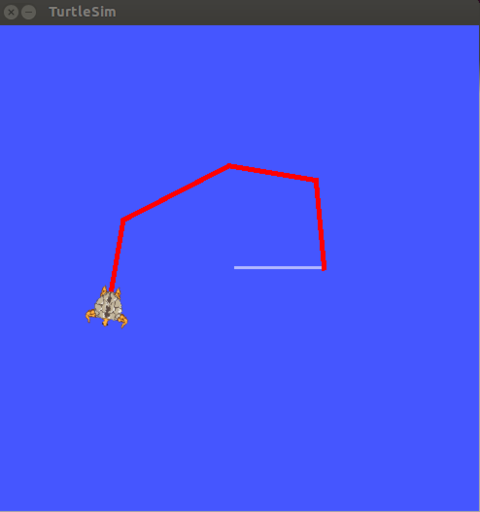
\includegraphics[width=0.5\columnwidth]{pictures/chapter5/rosservice_call.png}
\caption{rosservice call 예제}
\end{figure}

\newpage
%-------------------------------------------------------------------------------
\subsection{rosparam : ROS 매개변수}\index{rosparam : ROS 매개변수}

우선, 매개변수(parameter)\footnote{ROS, rosparam, http://wiki.ros.org/rosparam}에 대해서 이해하고 있어야 한다. 자세한 내용은 섹션~\nameref{sec:RosTerm}(pp.\pageref{def:RosParameter})에서 설명해두었다. 참고하도록 하자.

\vspace{\baselineskip}
\noindent
\begin{description}
\item[rosparam list] : 매개변수 목록 보기
\item[rosparam get 매개변수이름] : 매개변수 값 불러오기
\item[rosparam set 매개변수이름] : 매개변수 값 설정 
\item[rosparam dump 파일이름] : 매개변수를 지정한 파일에 저장한다
\item[rosparam load 파일이름] : 지정한 파일에 저장된 매개변수를 불러온다
\item[rosparam delete 매개변수이름] : 매개변수를 삭제한다 
\end{description}

\vspace{\baselineskip}
\noindent
※ 아래의 예제를 실행하기 전에 모든 노드를 종료하도록 하자. 그리고 난후, 각각 다른 터미널창에서 아래의 명령어를 실행하여 turtlesim\_node 및 turtle\_teleop\_key를 실행해주자.

\begin{lstlisting}[language=ROS]
roscore
rosrun turtlesim turtlesim_node 
rosrun turtlesim turtle_teleop_key
\end{lstlisting}

\setcounter{num}{0}

\noindent
\stepcounter{num}\circled{\thenum} rosparam list : 매개변수 목록 보기

\begin{lstlisting}[language=ROS]
$ rosparam list
/background_b
/background_g
/background_r
/rosdistro
/roslaunch/uris/host_192_168_4_185__39536
/rosversion
/run_id
\end{lstlisting}

\noindent
동일한 네트워크에서 사용중인 매개변수 목록이 표시된다.

\vspace{\baselineskip}
\noindent
\stepcounter{num}\circled{\thenum} rosparam get [매개변수이름] : 매개변수 값 불러오기

\begin{lstlisting}[language=ROS]
$ rosparam get /background_b
255
\end{lstlisting}

\noindent
특정 매개변수 값을 확인하고 싶을때는 위와 같이 "rosparam get" 명령어에 옵션으로 매개변수이름을 적어주면 된다.

\begin{lstlisting}[language=ROS]
$ rosparam get /
background_b: 255
background_g: 86
background_r: 69
rosdistro: 'hydro
  '
roslaunch:
  uris: {host_192_168_4_185__39536: 'http://192.168.4.185:39536/'}
rosversion: '1.9.50
  '
run_id: 93598b26-44f6-11e3-a077-d43d7e970cb0
\end{lstlisting}

\noindent
특정 매개변수가 아니라 모든 매개변수의 값을 확인하고 싶을 경우에는 옵션으로 "/" 를 붙여주면 위와같이 모든 매개변수의 값을 확인할 수 있다.

\vspace{\baselineskip}
\noindent
\stepcounter{num}\circled{\thenum} rosparam set [매개변수이름] : 매개변수 값 설정 

\begin{lstlisting}[language=ROS]
$ rosparam set background_b 0
$ rosservice call clear
\end{lstlisting}

\begin{figure}[h]
\centering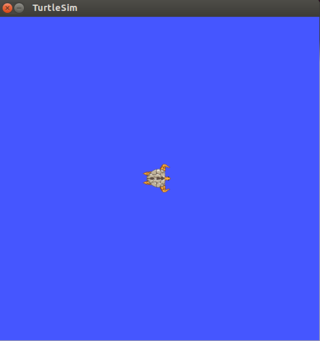
\includegraphics[width=0.4\columnwidth]{pictures/chapter5/rosparam_set1.png}
\centering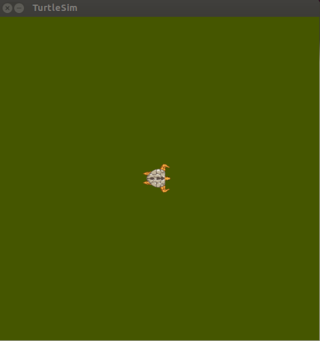
\includegraphics[width=0.4\columnwidth]{pictures/chapter5/rosparam_set2.png}
\caption{rosparam set 예제}
\end{figure}

\noindent
매개변수 값을 설정하는 명령어이다. 위 예제에서 "turtlesim" 노드의 배경색관련 매개변수인 "background\_b" 를 "0"으로 설정하였다. 그러면 rgb 는 255, 86, 69 에서 0, 86, 69 으로 변경되기에 위 오른쪽 그림처럼 짙은 녹색이 된다.

단, "turtlesim" 노드는 매개변수를 매번 읽는 것이 아니기에 "rosparam set background\_b 0" 명령어로 매개변수를 수정후에, "rosservice call clear" 명령어로 화면을 갱신해줘야한다. 이는 노드에 따라 매개변수 반영이 달라지게 된다.

\vspace{\baselineskip}
\noindent
\stepcounter{num}\circled{\thenum} rosparam dump [파일이름] : 매개변수를 지정한 파일에 저장한다

\begin{lstlisting}[language=ROS]
$ rosparam dump ~/parameters.yaml
\end{lstlisting}

\noindent
현재의 매개변수 값을 "parameters.yaml" 라는 파일에 저장하게 된다. 이는 매번 사용되는 매개변수값을 저장하여 다음 실행때에 사용할 수 있어서 매우 편리하다. (~/ 은 유저의 home 폴더를 의미한다)

\vspace{\baselineskip}
\noindent
\stepcounter{num}\circled{\thenum} rosparam delete [매개변수이름] : 매개변수를 삭제한다

\begin{lstlisting}[language=ROS]
$ rosparam delete /background_b
\end{lstlisting}

\noindent
지정한 매개변수를 삭제하는 명령어이다.

\newpage
%-------------------------------------------------------------------------------
\subsection{rosmsg : ROS 메시지 정보}\index{rosmsg : ROS 메시지 정보}

우선, 메시지(message)\footnote{ROS, rosmsg, http://wiki.ros.org/rosmsg}에 대해서 이해하고 있어야 한다. 자세한 내용은 섹션~\nameref{sec:RosTerm}(pp.\pageref{def:RosMessage})에서 설명해두었다. 참고하도록 하자.

\vspace{\baselineskip}
\noindent
\begin{description}
\item[rosmsg list] : 모든 메시지를 목록으로 표시한다
\item[rosmsg show 메시지이름] : 지정한 메시지 정보를 표시한다
\item[rosmsg md5 메시지이름] : md5sum을 표시한다
\item[rosmsg package 패키지이름] : 지정한 패키지에서 사용되는 메시지의 목록을 표시한다
\item[rosmsg packages] : 메시지를 사용하는 모든 패키지의 목록을 표시한다
\end{description}

\vspace{\baselineskip}
\noindent
※ 아래의 예제를 실행하기 전에 모든 노드를 종료하도록 하자. 그리고 난후, 각각 다른 터미널창에서 아래의 명령어를 실행하여 turtlesim\_node 및 turtle\_teleop\_key를 실행해주자.

\begin{lstlisting}[language=ROS]
$ roscore
$ rosrun turtlesim turtlesim_node 
$ rosrun turtlesim turtle_teleop_key
\end{lstlisting}

\setcounter{num}{0}

\vspace{\baselineskip}
\noindent
\stepcounter{num}\circled{\thenum} rosmsg list : 모든 메시지를 목록으로 표시한다

\begin{lstlisting}[language=ROS]
$ rosmsg list
actionlib/TestAction
actionlib/TestActionFeedback
actionlib/TestActionGoal
actionlib/TestActionResult
actionlib/TestFeedback
actionlib/TestGoal
sensor_msgs/Joy
sensor_msgs/JoyFeedback
sensor_msgs/JoyFeedbackArray
sensor_msgs/LaserEcho
zeroconf_msgs/DiscoveredService
...
\end{lstlisting}

\noindent
현재 ROS에 포함되어 있는 패키지에 따라 결과값이 틀려질 수 있다. 이 명령어는 현재 ROS에 설치된 패키지의 모든 메시지를 목록으로 표시하게 된다.

\vspace{\baselineskip}
\noindent
\stepcounter{num}\circled{\thenum} rosmsg show [메시지이름] : 지정한 메시지 정보를 표시한다

\begin{lstlisting}[language=ROS]
$ rosmsg show turtlesim/Pose 
float32 x
float32 y
float32 theta
float32 linear_velocity
float32 angular_velocity
\end{lstlisting}

\noindent
지정한 메시지 정보를 표시한다. 위 예제에서는 "turtlesim/Pose" 라는 이름의 메시지의 정보를 출력해보았다. float32 부동소수점형 변수로 x, y, theta, linear\_velocity, angular\_velocity 의 5개의 정보가 포함되어 있는 메시지임을 확인할 수 있다.

\vspace{\baselineskip}
\noindent
\stepcounter{num}\circled{\thenum} rosmsg md5 [메시지이름] : md5sum\footnote{섹션~\nameref{sec:RosTerm}(pp.\pageref{def:RosMD5})}을 표시한다

\begin{lstlisting}[language=ROS]
$ rosmsg md5 turtlesim/Pose 
863b248d5016ca62ea2e895ae5265cf9
\end{lstlisting}

\noindent
"turtlesim/Pose" 라는 이름의 메시지의 md5 정보를 확인한다. 간혹 메시지 통신중에 MD5 문제가 발생된다면 md5sum 을 확인할 필요가 있는데 이때에 사용되는 명령어이다. 일반적으로 많이 사용되지는 않는다.

\vspace{\baselineskip}
\noindent
\stepcounter{num}\circled{\thenum} rosmsg package [패키지이름] : 지정한 패키지에서 사용되는 메시지의 목록을 표시한다

\begin{lstlisting}[language=ROS]
$ rosmsg package turtlesim 
turtlesim/Color
turtlesim/Pose
\end{lstlisting}

\noindent
특정 패키지에서 사용되는 메시지들을 확인할 수 있다.

\vspace{\baselineskip}
\noindent
\stepcounter{num}\circled{\thenum} rosmsg packages : 메시지를 사용하는 모든 패키지의 목록을 표시한다

\begin{lstlisting}[language=ROS]
$ rosmsg packages
actionlib
actionlib_msgs
actionlib_tutorials
base_local_planner
bond
control_msgs
costmap_2d
\end{lstlisting}

%-------------------------------------------------------------------------------
\subsection{rossrv : ROS 서비스 정보}\index{rossrv : ROS 서비스 정보}

우선, 서비스(service)\footnote{ROS, rosmsg, http://wiki.ros.org/rosmsg}에 대해서 이해하고 있어야 한다. 자세한 내용은 섹션~\nameref{sec:RosTerm}(pp.\pageref{def:RosService})에서 설명해두었다. 참고하도록 하자.

\vspace{\baselineskip}
\noindent
\begin{description}
\item[rossrv list] : 모든 서비스를 목록으로 표시한다
\item[rossrv show 서비스이름] : 지정한 서비스 정보를 표시한다
\item[rossrv md5 서비스이름] : md5sum을 표시한다
\item[rossrv package 패키지이름] : 지정한 패키지에서 사용되는 서비스의 목록을 표시한다
\item[rossrv packages] : 서비스를 사용하는 모든 패키지의 목록을 표시한다
\end{description}

\vspace{\baselineskip}
\noindent
※ 아래의 예제를 실행하기 전에 모든 노드를 종료하도록 하자. 그리고 난후, 각각 다른 터미널창에서 아래의 명령어를 실행하여 turtlesim\_node 및 turtle\_teleop\_key를 실행해주자.

[leftmargin=*]
\begin{lstlisting}[language=ROS]
roscore
rosrun turtlesim turtlesim_node 
rosrun turtlesim turtle_teleop_key
\end{lstlisting}

\setcounter{num}{0}

\vspace{\baselineskip}
\noindent
\stepcounter{num}\circled{\thenum} rossrv list : 모든 서비스를 목록으로 표시한다

\begin{lstlisting}[language=ROS]
$ rossrv list
control_msgs/QueryCalibrationState
control_msgs/QueryTrajectoryState
diagnostic_msgs/SelfTest
dynamic_reconfigure/Reconfigure
gazebo_msgs/ApplyBodyWrench
gazebo_msgs/ApplyJointEffort
gazebo_msgs/BodyRequest
gazebo_msgs/DeleteModel
...
\end{lstlisting}

\noindent
현재 ROS에 포함되어 있는 패키지에 따라 결과값이 틀려질 수 있다. 이 명령어는 현재 ROS에 설치된 패키지의 모든 서비스를 목록으로 표시하게 된다.

\vspace{\baselineskip}
\noindent
\stepcounter{num}\circled{\thenum} rossrv show [서비스이름] : 지정한 서비스 정보를 표시한다

\begin{lstlisting}[language=ROS]
$ rossrv md5 turtlesim/SetPen 
9f452acce566bf0c0954594f69a8e41b
\end{lstlisting}

\noindent
"turtlesim/SetPen" 라는 이름의 서비스의 md5 정보를 확인한다. 간혹 서비스 요청 중에 MD5 문제가 발생된다면 md5sum 을 확인할 필요가 있는데 이때에 사용되는 명령어이다. 일반적으로 많이 사용되지는 않는다.

\vspace{\baselineskip}
\noindent
\stepcounter{num}\circled{\thenum} rossrv package [패키지이름] : 지정한 패키지에서 사용되는 서비스의 목록을 표시한다

\begin{lstlisting}[language=ROS]
$ rossrv package turtlesim 
turtlesim/Kill
turtlesim/SetPen
|turtlesim/Spawn
turtlesim/TeleportAbsolute
turtlesim/TeleportRelative
\end{lstlisting}

\noindent
특정 패키지에서 사용되는 메시지들을 확인할 수 있다.

\vspace{\baselineskip}
\noindent
\stepcounter{num}\circled{\thenum} rossrv packages : 서비스를 사용하는 모든 패키지의 목록을 표시한다

\begin{lstlisting}[language=ROS]
$ rossrv packages
control_msgs
diagnostic_msgs
dynamic_reconfigure
gazebo_msgs
map_msgs
nav_msgs
navfn
nodelet
oroca_ros_tutorials
roscpp
sensor_msgs
std_srvs
tf
tf2_msgs
turtlesim
\end{lstlisting}

%-------------------------------------------------------------------------------
\subsection{rosbag : ROS 로그 정보}\index{rosbag : ROS 로그 정보}
\label{subsub:Rosbag}

우선, 배그(bag)\footnote{ROS, rosbag, http://wiki.ros.org/rosbag}\footnote{ROS, Bags Format, http://wiki.ros.org/Bags/Format}에 대해서 이해하고 있어야 한다. 자세한 내용은 섹션~\nameref{sec:RosTerm}(pp.\pageref{def:RosBag})에서 설명해두었다. 참고하도록 하자.

\vspace{\baselineskip}
\noindent
\begin{description}
\item[rosbag record 옵션 토픽이름] : 지정한 토픽의 메시지를 기록한다
\item[rosbag info bag파일이름] : 배그파일의 정보를 확인한다
\item[rosbag play bag파일이름] : 지정한 배그파일을 재생한다

\item[rosbag compress bag파일이름] : 지정한 배그파일을 압축한다
\item[rosbag decompress bag파일이름] : 지정한 배그파일을 압축해제한다

\item[rosbag filter 입력bag파일 출력bag파일 옵션] : 지정된 내용을 제거한 새로운 bag 파일을 생성한다
\item[rosbag reindex bag파일이름] : 인덱스를 재색인한다

\item[rosbag check bag파일이름] : 지정한 배그파일이 현재 시스템에서 재생 가능한지 확인한다
\item[rosbag fix 입력bag파일 출력bag파일 옵션] : 버전이 다른 재생 불가능 bag파일을 재생가능하게 수정한다
\end{description}

\vspace{\baselineskip}
\noindent
※ 아래의 예제를 실행하기 전에 모든 노드를 종료하도록 하자. 그리고 난후, 각각 다른 터미널창에서 아래의 명령어를 실행하여 turtlesim\_node 및 turtle\_teleop\_key를 실행해주자.

\vspace{\baselineskip}
\begin{lstlisting}[language=ROS]
roscore
rosrun turtlesim turtlesim_node 
rosrun turtlesim turtle_teleop_key
\end{lstlisting}

\setcounter{num}{0}

\noindent
\stepcounter{num}\circled{\thenum} rosbag record [옵션] [토픽이름] : 지정한 토픽의 메시지를 기록한다

\begin{lstlisting}[language=ROS]
$ rostopic list
/rosout
/rosout_agg
/turtle1/cmd_vel
/turtle1/color_sensor
/turtle1/pose
\end{lstlisting}

\noindent
우선, "rostopic list" 명령어를 이용하여 현재 ROS 네트워크에서 사용중인 토픽 목록을 확인한다.

\begin{lstlisting}[language=ROS]
$ rosbag record /turtle1/cmd_vel
[ INFO] [1383546556.032289494]: Subscribing to /turtle1/cmd_vel
[ INFO] [1383546556.035616801]: Recording to 2013-11-04-15-29-16.bag.
\end{lstlisting}

\noindent
사용중인 토픽중에서 기록하고자 하는 토픽을 옵션으로 입력하여 bag기록을 시작한다. 기록을 시작한 후, "turtle\_teleop\_key" 노드에서 키보드로 명령을 내리면서 거북이를 이동시켜본다. 이때에 사용된 "/turtle1/cmd\_vel" 토픽이 기록되게 된다. 기록 종료는 Ctrl + C 으로 종료하면 된다. 위 정보처럼 "2013-11-04-15-29-16.bag" 와 같은 .bag 파일이 생성될 것이다.

\newpage

\begin{figure}[h]
\centering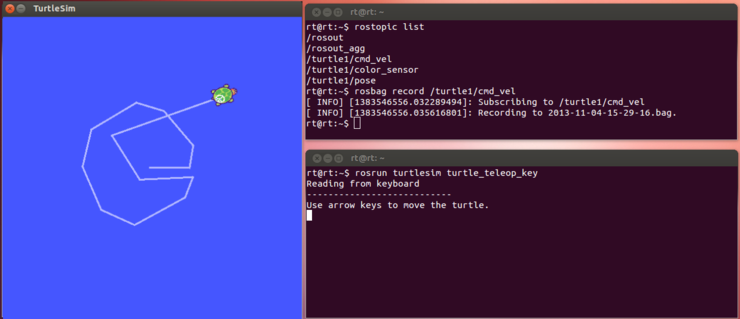
\includegraphics[width=0.8\columnwidth]{pictures/chapter5/rosbag_record.png}
\caption{rosbag record 예제}
\end{figure}

\begin{lstlisting}[language=ROS]
$ rosbag record -a
[ INFO] [1383547478.578148917]: Recording to 2013-11-04-15-44-38.bag.
[ INFO] [1383547479.577915716]: Subscribing to /turtle1/color_sensor
[ INFO] [1383547479.578655855]: Subscribing to /rosout
[ INFO] [1383547479.579363447]: Subscribing to /rosout_agg
[ INFO] [1383547479.579924366]: Subscribing to /turtle1/cmd_vel
[ INFO] [1383547479.580483400]: Subscribing to /turtle1/pose
\end{lstlisting}

\noindent
특정 토픽이 아닌 모든 토픽을 기록하고 싶다면 위와 같이 옵션에 "-a" 를 붙여주면 모든 토픽이 동시에 기록된다.

\vspace{\baselineskip}
\noindent
\stepcounter{num}\circled{\thenum} rosbag info [bag파일이름] : 배그파일의 정보를 확인한다

\begin{lstlisting}[language=ROS]
$ rosbag info 2013-11-04-15-29-16.bag 
path:        2013-11-04-15-29-16.bag
version:     2.0
duration:    16.9s
start:       Nov 04 2013 15:29:19.83 (1383546559.83)
end:         Nov 04 2013 15:29:36.74 (1383546576.74)
size:        23.1 KB
messages:    173
compression: none [1/1 chunks]
types:       geometry_msgs/Twist [9f195f881246fdfa2798d1d3eebca84a]
topics:      /turtle1/cmd_vel   173 msgs    : geometry_msgs/Twist
\end{lstlisting}

\noindent
배그파일의 정보를 확인할 수 있다. 위의 예제에서는 "/turtle1/cmd\_vel" 토픽을 기록하였으며, 총 173개의 메시지가 기록되었다. 사용된 메시지 형태는 "geometry\_msgs/Twist" 이며, 그이외에도 경로, bag 버전, 시간 등의 정보를 확인 할 수 있다.

\vspace{\baselineskip}
\noindent
\stepcounter{num}\circled{\thenum} rosbag play [bag파일이름] : 지정한 배그파일을 재생한다

\begin{lstlisting}[language=ROS]
$ rosbag play 2013-11-04-15-29-16.bag 
[ INFO] [1383548100.180862433]: Opening 2013-11-04-15-29-16.bag

Waiting 0.2 seconds after advertising topics... done.

Hit space to toggle paused, or 's' to step.
[RUNNING]  Bag Time: 1383546576.681423   Duration: 16.855905 / 16.918187     
Done.
\end{lstlisting}

\noindent
기록해둔 "2013-11-04-15-29-16.bag" 를 재생하는 명령어이다. 아래의 그림처럼 원본과 재생시의 데이터가 같음을 확인할 수 있다.

\begin{figure}[h]
\centering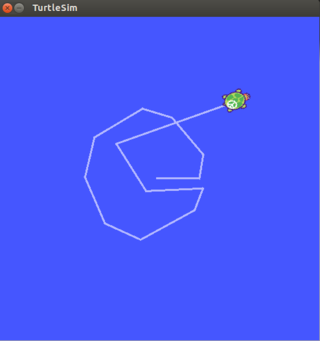
\includegraphics[width=0.4\columnwidth]{pictures/chapter5/rosbag_play1.png}
\centering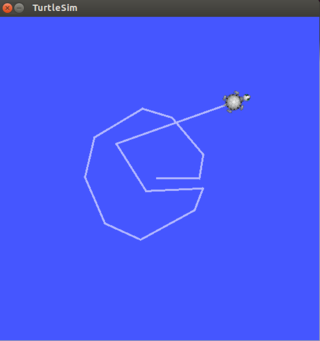
\includegraphics[width=0.4\columnwidth]{pictures/chapter5/rosbag_play2.png}
\caption{rosbag play 예제}
\end{figure}

\vspace{\baselineskip}
\noindent
\stepcounter{num}\circled{\thenum} rosbag compress [bag파일이름] : 지정한 배그파일을 압축한다

\begin{lstlisting}[language=ROS]
$ rosbag compress 2013-11-04-15-29-16.bag 
 2013-11-04-15-29-16.bag                     100%             16.4 KB 00:00  
\end{lstlisting}

\noindent
짧은 시간의 배그파일은 경우에는 그다지 용량이 크지 않아 문제 없지만, 장시간의 데이터를 기록할시에는 저장공간을 많이 차지한다. 위 압축 명령은 이럴때 사용하는 명령어로 압축해놓으면 매우 적은 저장 공간을 차지하게 된다. 위의 예제에서는 아래와 같이 1/3로 축소되었다. 그리고, 압축전 원본 파일은 orig라는 이름이 추가되어 별도로 저장된다.

\vspace{\baselineskip}
\noindent
/home/rt/2013-11-04-15-29-16.bag 8.6kB\\
/home/rt/2013-11-04-15-29-16.orig.bag 23.7kB

\vspace{\baselineskip}
\noindent
\stepcounter{num}\circled{\thenum} rosbag decompress [bag파일이름] : 지정한 배그파일을 압축해제한다

\begin{lstlisting}[language=ROS]
$ rosbag decompress 2013-11-04-15-29-16.bag 
2013-11-04-15-29-16.bag                     100%             16.3 KB 00:00  
\end{lstlisting}

\noindent
압축해제시에는 위의 명령어를 이용하면 된다. 압축전 상태로 원상 복귀된다.


% rosbag filter [입력bag파일] [출력bag파일] [옵션] : 지정된 내용을 제거한 새로운 bag 파일을 생성한다
% rosbag reindex [bag파일이름] : 인덱스를 재색인한다
% rosbag check [bag파일이름] : 지정한 배그파일이 현재 시스템에서 재생 가능한지 확인한다
% rosbag fix [입력bag파일] [출력bag파일] [옵션] : 버전이 다른 재생 불가능 bag파일을 재생가능하게 수정한다

%-------------------------------------------------------------------------------
% -*- root: main.tex -*-
%-------------------------------------------------------------------------------
\chapterimage{chapter_head_6.pdf} 

%-------------------------------------------------------------------------------
\chapter{ROS 도구}

%-------------------------------------------------------------------------------
\section{ROS 도구 (RViz)}\index{ROS 도구 (RViz)}

ROS는 "로봇 운영체제 강좌 : ROS 명령어" 에서 설명한 커맨드형 명령어 이외에도 ROS 활용에 필요한 다양한 도구들이 존재한다. 이는 커맨드형 명령어와 상호보완하는 형태로 ROS 유저들에게는 필수적으로 알아둬야 할 부분이다.

ROS 도구로는 ROS 유저들이 개인적으로 공개한 툴까지 포함하여 상당히 많은 수가 있는데 그 중에서 이번 강좌에서는 1) 3차원 시각화를 돕는 RViz\footnote{ROS wiki, RViz, http://wiki.ros.org/rviz}\footnote{ROS wiki, RViz User Guide, http://wiki.ros.org/rviz/UserGuide}, 2) 데이터 로깅 툴인 rqt\_bag\footnote{ROS wiki, RQT Bag, http://wiki.ros.org/rqt\_bag}, 3) 데이터 플롯 툴인 rqt\_plot\footnote{ROS wiki, RQT Plot, http://wiki.ros.org/rqt\_plot}. 4) 노드간의 관계 및 메시지를 확인 가능한 rqt\_graph\footnote{ROS wiki, RQT Graph, http://wiki.ros.org/rqt\_graph} , 5) GUI 통합 툴인 rqt\footnote{ROS wiki, RQT, http://wiki.ros.org/rqt} 을 알아볼 것이다. 있다. 이들 툴들은 ros와의 직접적인 처리를 행하는 것은 아니지만 ROS를 이용한 프로그래밍에 매우 유용한 보조툴이다. 

특히, ROS Fuerte 버전부터는 RViz는 rqt 라는 이름으로 rqt\_bag, rqt\_plot, rqt\_graph 등과 함께 36가지 플러그인이 통폐합되어 종합 GUI 툴로써 사용 가능해졌다. 그뿐만 아니라 rqt는 QT로 개발되어 있기 때문에 유저들이 자유롭게 플러그인을 개발하여 추가할 수도 있어서 매우 편리하다. 이번 강좌에서는 아래의 내용에 대해서 알아보도록 하자.

\begin{itemize}[leftmargin=*]
\item RViz : 3D visualization tool / 3차원 시각화 툴
\item rqt\_bag : Logging and Visualization Sensor Data, rosbag gui tool / 메시지 기록 GUI 유틸리티
\item rqt\_plot : Data Plot Tool / 2차원 데이터 플롯 툴 
\item rqt\_graph : 노드 및 메시지간의 상관 관계를 그래프로 나타내는 툴
\item rqt : QT 기반의 ROS GUI 개발 툴
\end{itemize}

%-------------------------------------------------------------------------------
\subsection{RViz 개요 및 활용}\index{RViz 개요 및 활용}

RViz는 ROS의 3차원 시각화 툴이다. ROS 네트워크상의 데이터를 3차원으로 표시하는 것이 주요 목적으로 센서 데이터를 시각화하여 확인할 수 있다. 

예를들어, 레이저 레인지 파인더(LRF: Laser Range Finder)의 센서로부터의 장애물과의 거리값, Kinect 및 Xtion과 같은 3차원 거리 센서의 포인트 클라우드 데이터 (PCD: Point Cloud Data), 카메라로부터 취득한 컬러 이미지 값 등을 실시간으로 표시할 수 있다. 

또한, 사용자가 지정한 폴리곤을 이용하여 각종 표시를 지원하고 있다. 특히, Interactive Markers 를 이용하여 사용자 노드로부터의 명령 및 데이터를 수신하여 상호호환적인 움직을 나타낼 수도 있다. 더불어, XML로 URDF(Unified Robot Description Format) 을 작성하여 로봇을 3차원 모델로 표현하고, 각각의 모델은 자유도에 따라 이동 및 구동 가능하도록 할 수 있어서 시뮬레이션 및 실시간 제어에 확인용으로 사용가능하다.

그 이외에 필자가 작성한 패키지중 RViz를 이용하여 표시가능한것을 아래에 링크하였다. 참고하길 바란다.

\begin{figure}[h]
\centering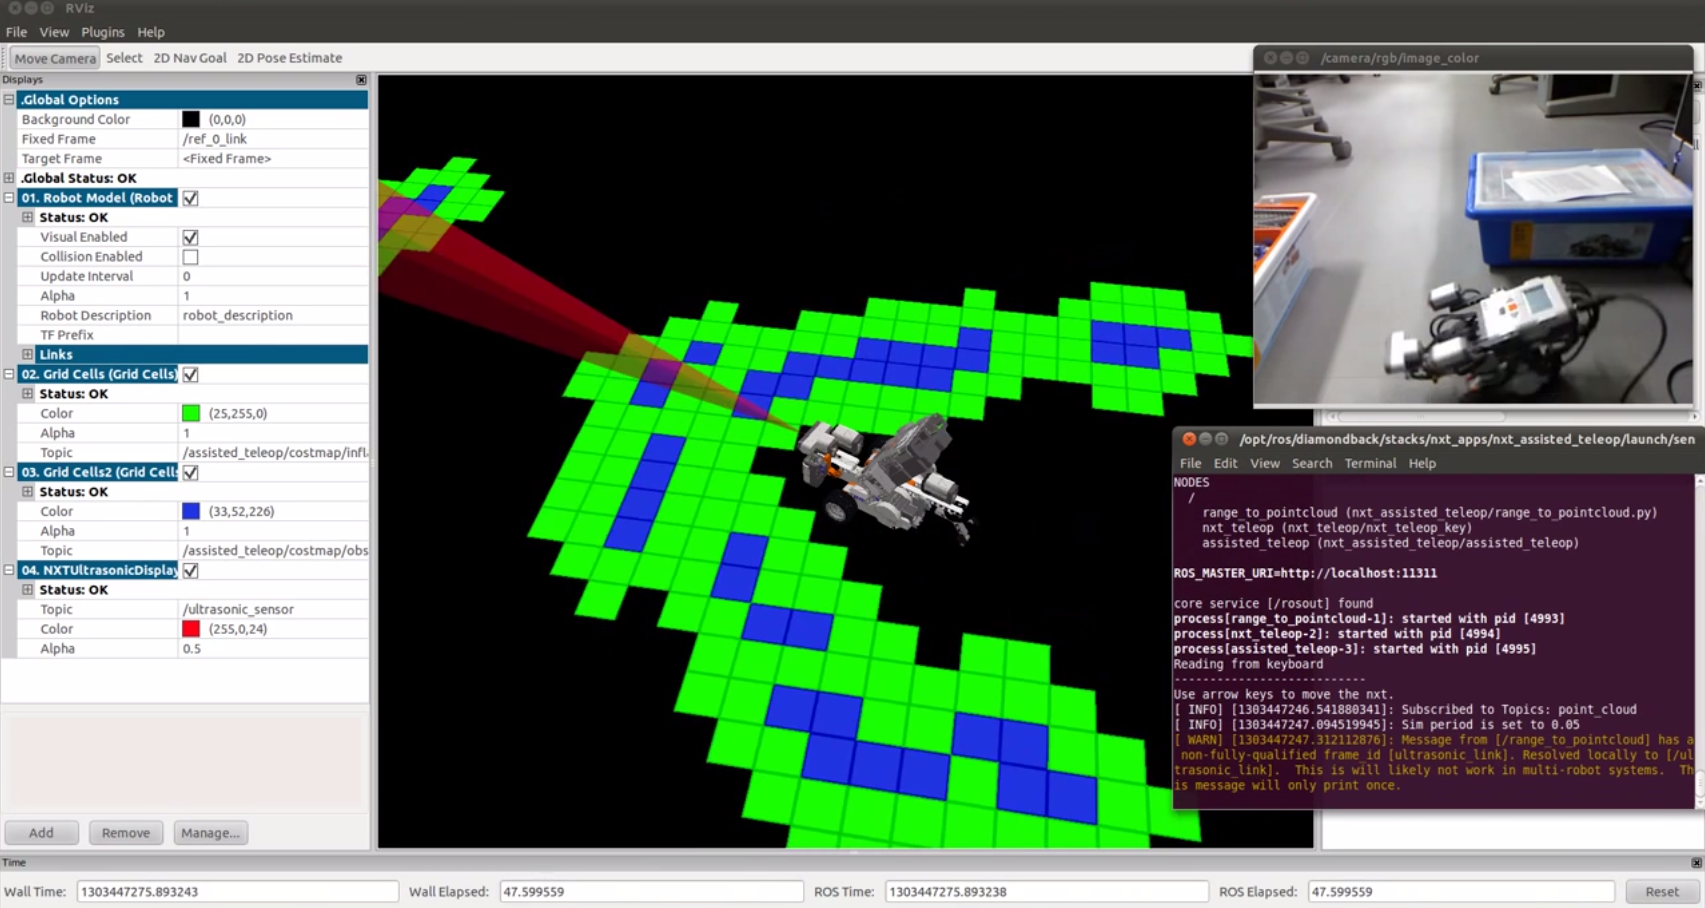
\includegraphics[width=0.7\columnwidth]{pictures/chapter6/rviz_example1.png}
\caption{RViz의 사용예1) 레고를 이용한 모바일 로봇과 초음파 센서를 이용하여 간단한 맵작성}
\end{figure}

\begin{figure}[h]
\centering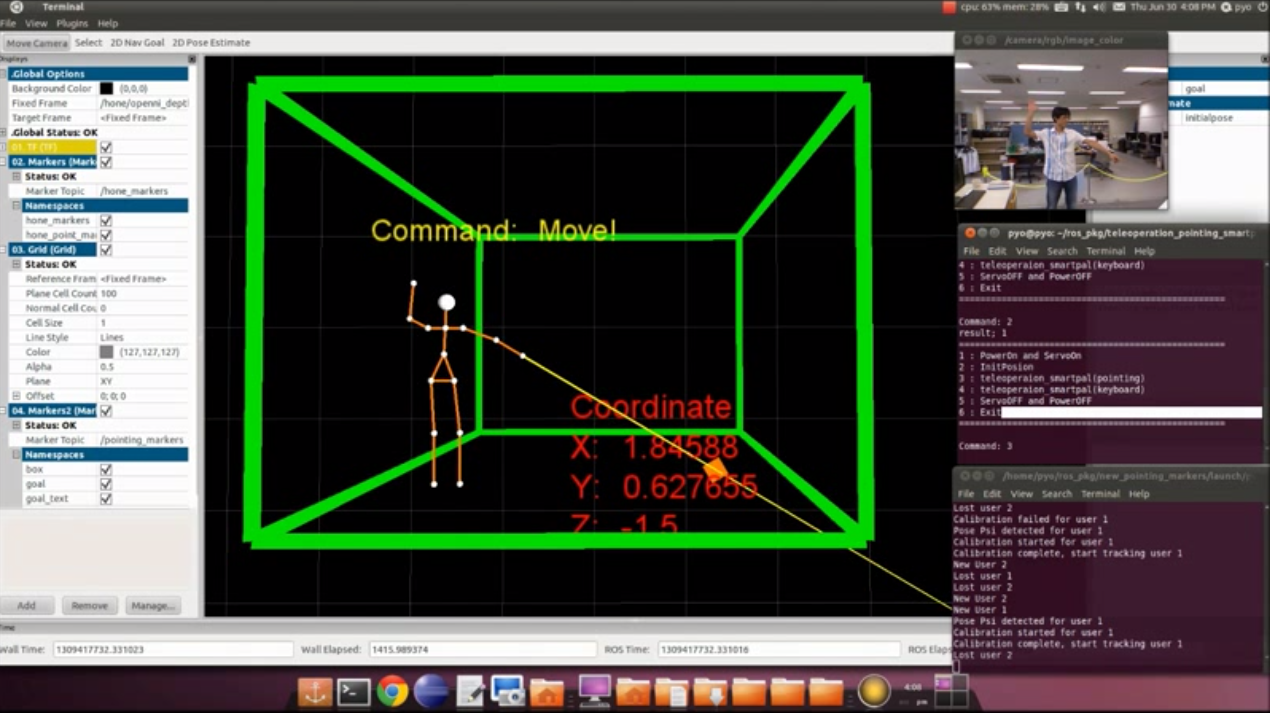
\includegraphics[width=0.7\columnwidth]{pictures/chapter6/rviz_example2.png}
\caption{RViz의 사용예2) 키넥트로부터 사람의 골격을 취득하고 로봇을 제어하는 모습}
\end{figure}

%-------------------------------------------------------------------------------
\subsection{RViz 설치 및 실행}\index{RViz 설치 및 실행}

ROS 설치시에 기본 설치라고도 부를 수 있는 "Desktop-Full Install" 를 설치하게되면 RViz는 기본적으로 설치되어 있다. 만약에 "Desktop-Full Install" 으로 설치하지 않았거나, RViz 가 설치되어 있지 않을 경우에는 아래의 명령어로 설치할 수있다.

\begin{lstlisting}[language=bash]
sudo apt-get install ros-indigo-rviz
\end{lstlisting}

\noindent
RViz 의 실행 명령어는 아래와 같다. (단, roscore 가 실행되어 있어야 한다.)

\begin{lstlisting}[language=bash]
rosrun rviz rviz
\end{lstlisting}

%-------------------------------------------------------------------------------
\subsection{RViz 화면 구성}\index{RViz 화면 구성}

\begin{figure}[h]
\centering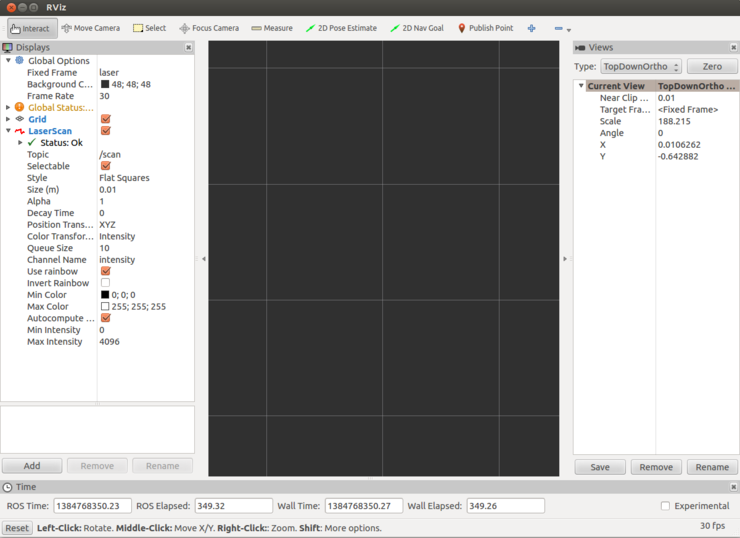
\includegraphics[width=0.8\columnwidth]{pictures/chapter6/rviz.png}
\caption{RViz 화면 구성}
\end{figure}

\begin{enumerate}[leftmargin=*, label=\arabic{*})]
\item 3D 뷰 (3D view)
: 위 화면의 가운데의 검정색 부분을 가르킨다. 각종 데이타를 3차원으로 볼 수 있는 메인 화면이다.

\item 디스플레이(Displays) 
: 왼쪽에 있는 디스플레이 화면은 각종 토픽으로부터 사용자가 원하는 데이타의 뷰를 선택하는 화면이다.

\item 메뉴 (Menu)
: 메뉴는 상단에 놓여져 있다. 현재의 뷰 상태를 저장하거나 읽어오는 명령, 각종 패널의 뷰 옵션을 체크할 수 있다.

\item 툴 (Tools)
: 대부분 네비게이션에 필요한 툴들이 놓여져 있다. 상세한 설명은 네비게이션을 다룰때 설명하도록 하겠다.

\item 뷰 (Views)
: 3D 뷰의 시점을 변경한다.

\item 시간 (Time)
: 현재 시간과 ROS Time 을 실시간으로 보여준다.
\end{enumerate}

%-------------------------------------------------------------------------------
% \subsection{사용 방법}\index{사용 방법}

%-------------------------------------------------------------------------------
\subsection{데이터 표시의 예}\index{데이터 표시의 예}

\begin{figure}[h]
\centering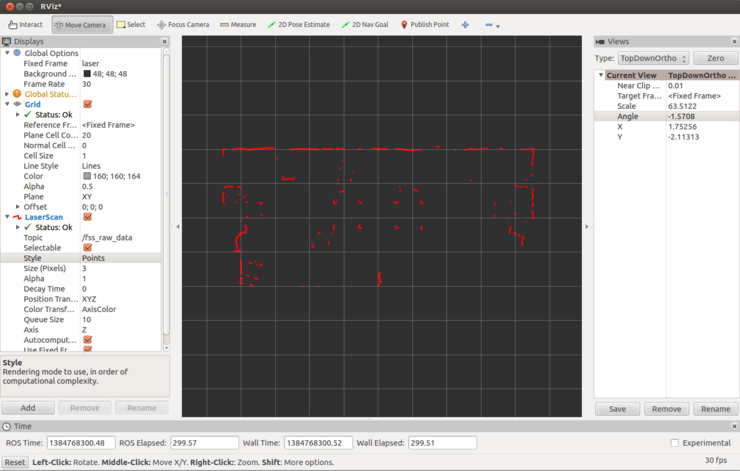
\includegraphics[width=0.7\columnwidth]{pictures/chapter6/rviz_example3.png}
\caption{RViz 사용예3) LRF를 이용한 거리측정}
\end{figure}

\begin{figure}[h]
\centering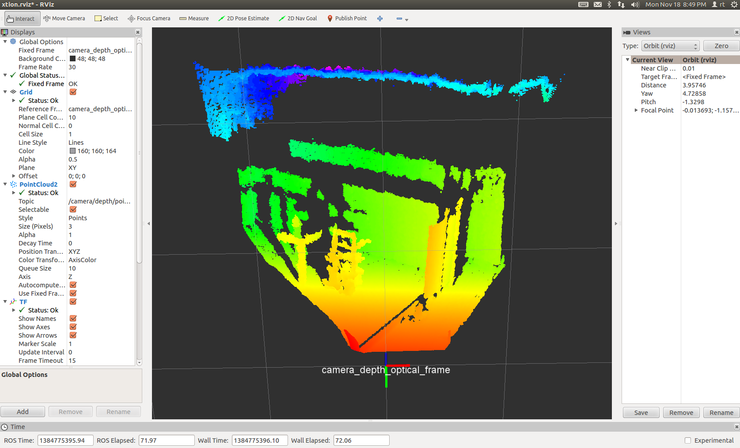
\includegraphics[width=0.7\columnwidth]{pictures/chapter6/rviz_example4.png}
\caption{RViz 사용예4) Xtion 센서로부터 취득한 3차원 거리 값}
\end{figure}

\begin{figure}[h]
\centering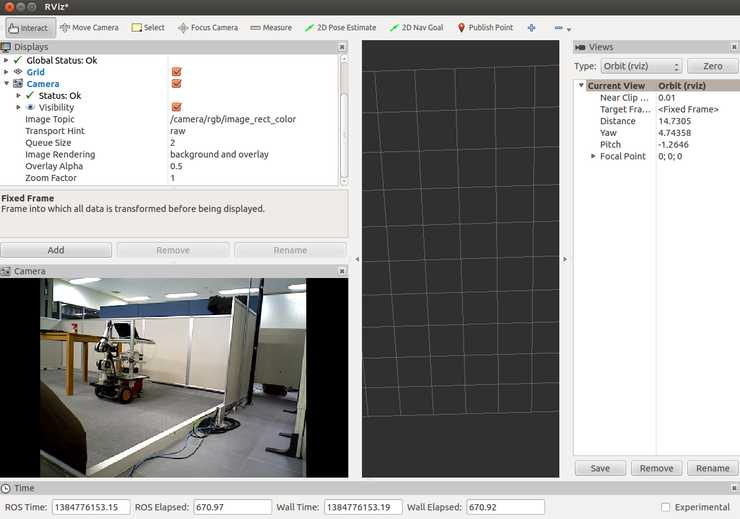
\includegraphics[width=0.7\columnwidth]{pictures/chapter6/rviz_example5.png}
\caption{RViz 사용예5) Xtion 센서에 장착된 카메라를 이용한 이미지 데이터 취득}
\end{figure}

%-------------------------------------------------------------------------------
\section{ROS 도구 (rqt) }\index{ROS 도구 (rqt) }

%-------------------------------------------------------------------------------
\subsection{rqt 개요}\index{rqt 개요}

ROS Fuerte 버전부터는 rqt 라는 이름으로 기존의 rxbag, rxplot, rxgraph 등이 통폐합되어 rqt\_bag, rqt\_plot, rqt\_graph 등을 플러그인으로 하는 종합 GUI 툴로써 사용 가능해졌다. 더불어, rviz 또한 rqt의 플러그인으로 편입되면서 rqt 는 ROS에서 빼놓을 수 없는 중요한 GUI 툴이 되었다. 그뿐만 아니라 rqt는 QT로 개발되어 있기 때문에 유저들이 자유롭게 플러그인을 개발하여 추가할 수도 있어서 매우 편리하다. 이번 강좌에서는 rqt의 대표적인 플러그인인 rqt\_bag, rqt\_plot, rqt\_graph 등 에 대해서 알아보도록 하겠다.

참고로, 그 이외에도 rqt\_action, rqt\_gui, rqt\_plot, rqt\_runtime\_monitorrqt\_bag, rqt\_gui\_cpp, rqt\_pose\_view, rqt\_rvizrqt\_bag\_plugins, rqt\_gui\_py, rqt\_publisher, rqt\_service\_callerrqt\_capabilities, rqt\_image\_view, rqt\_py\_common, rqt\_shellrqt\_console, rqt\_launch, rqt\_py\_console, rqt\_srvrqt\_controller\_manager, rqt\_logger\_level, rqt\_reconfigure, rqt\_tf\_treerqt\_dep, rqt\_moveit, rqt\_robot\_dashboard, rqt\_toprqt\_ez\_publisher, rqt\_msg, rqt\_robot\_monitor, rqt\_topicrqt\_graph, rqt\_nav\_view, rqt\_robot\_steering, rqt\_web 등의 플러그인이 존재한다.\sloppy

%-------------------------------------------------------------------------------
\subsection{rqt 설치}\index{rqt 설치}

ROS 설치시에 기본 설치라고도 부를 수 있는 "Desktop-Full Install" 를 설치하게되면 rqt는 기본적으로 설치되어 있다. 만약에 "Desktop-Full Install" 으로 설치하지 않았거나, rqt 가 설치되어 있지 않을 경우에는 아래의 명령어로 설치할 수있다.

\begin{lstlisting}[language=bash]
sudo apt-get install ros-indigo-rqt ros-indigo-rqt-common-plugins
\end{lstlisting}

추가로, rqt\_graph 에서는 그래프 생성을 위하여 추가적으로 설치해야할 파일이 있다. rqt\_graph 에서는 PyQtGraph, MatPlot, QwtPlot 을 지원하는데 우리는 rqt\_graph 가 추천하는 PyQtGraph 을 사용하도록 하자.

http://www.pyqtgraph.org/downloads/python-pyqtgraph\_0.9.8-1\_all.deb 에서 deb 파일을 받고 클릭하여 설치하도록 하자. 그 뒤 아래와 같이 rqt\_graph를 실행한 후, 프로그램의 오른쪽 상단에 있는 옵션을 의미하는 "기어" 모양의 아이콘을 클릭하면 아래의 첨부 그림과 같이 옵션을 선택할 수 있는데 PyQtGraph 를 선택해주면 된다. PyQtGraph 이외에도 MatPlot, QwtPlot 도 이용 가능하니 원하는 그래프 관련 라이브러리를 이용하면 된다.

\begin{lstlisting}[language=bash]
rqt_graph
\end{lstlisting}

\begin{figure}[h]
\centering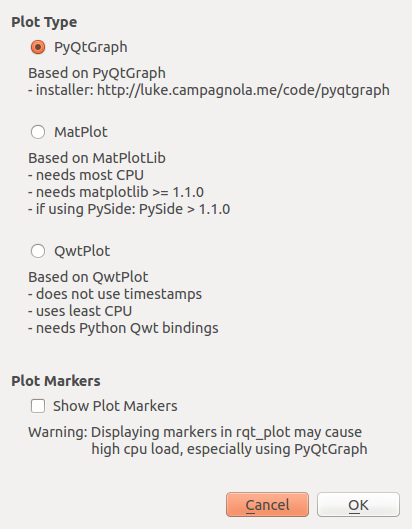
\includegraphics[width=0.5\columnwidth]{pictures/chapter6/rqtplotoption.png}
\caption{rqt\_graph의 설치 옵션}
\end{figure}

%-------------------------------------------------------------------------------
\subsection{rqt 실행 및 각 메뉴 소개}\index{rqt 실행 및 각 메뉴 소개}

실행은 아래와 같다. 단순히 rqt 라고 실행해주면 된다. (정식 실행명령어는 rosrun rqt\_gui rqt\_gui 이다)

\begin{lstlisting}[language=bash]
rqt
\end{lstlisting}

rqt 를 실행해주면 아래와 같이 rqt gui 화면이 나온다.처음 구동하였다면 아무런 표시가 없이 덩그러니 메뉴만 표시된다. 이는 rqt가 직접적으로 수행하는 프로그램인 플러그인이 지정되지 않았기 때문이다. 메뉴를 간단히 설명하자면, File의 경우, 단순히 rqt를 종료하는 서브메뉴만 있다. 플러그인(Plugins) 에는 27가지의 플러그인이 있다. 이를 선택하여 이용하게 된다. 동작(Running) 은 현재 동작중인 플러그인이 표시되어 필요치 않을시에 동작을 중단시킬 수 있는 메뉴이다. 끝으로 시각(Perspectives)은 현재 구동중인 플러그인을 셋트로 다음에도 같은 셋트를 이용하고 싶을때 저장하여 동일한 플러그인들을 실행할때 쓰는 메뉴이다.

\begin{figure}[h]
\centering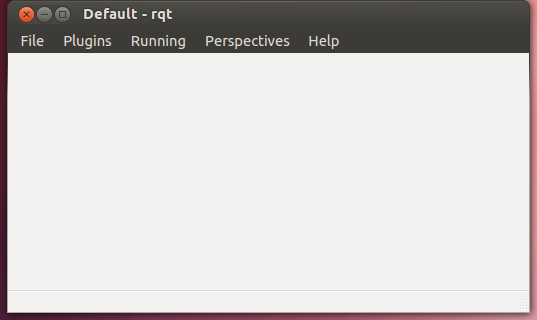
\includegraphics[width=0.6\columnwidth]{pictures/chapter6/rqt.png}
\caption{rqt의 초기 화면}
\end{figure}

%-------------------------------------------------------------------------------
\subsection{rqt 플러그인}\index{rqt 플러그인}

rqt의 상단 메뉴중에서 플러그인(Plugins)\footnote{ROS wiki, Plugins, http://wiki.ros.org/rqt/Plugins}\footnote{ROS wiki, RQT Common Plugins, http://wiki.ros.org/rqt\_common\_plugins}을 선택하면 27가지의 플러그인을 확인할 수 있다. 이 플러그인은 아래의 역할을 담당한다. 대부분 매우 필요한 기능등을 갖춘 rqt 의 기본 플러그인이다. 필요에 의해서 사용자가 개발한 플러그인도 추가 가능하다.

\subsubsection{액션 (Action)}
Action Type Browser | Action 타입의 데이터 구조를 확인하는 플러그인 
\subsubsection{구성 (Configuration)}
Dynamic Reconfigure | 노드들에서 제공하는 설정값 변경을 위한 GUI 설정값 변경 플러그인\\
Launch | roslaunch 의 GUI 플러그인, 로스런치의 이름 및 구성이 생각안날때 매우 유용하다.\\
\subsubsection{내성 (Introspection)}
Node Graph | 구동중인 모든 노드들의 관계도 및 메시지의 흐름을 확인할 수 있는 그래프 뷰 형식의 플러그인\\
Package Graph | 노드의 의존 관계를 표시하는 그래프 뷰 형식의 플러그인\\
Process Monitor | 현재 실행중인 노드들의 CPU사용률, 메모리사용륭, 스레드수 등을 확인 가능하다.\\
\subsubsection{로깅 (Logging)}
Bag | ROS 데이터 로깅 관련 플러그인\\
Console | 노드들에서 발생되는 경고(Warning), 에러(Error) 등의 메시지들을 한 화면에서 확인 가능한 플러그인\\
Logger Level | ROS의 Debug, Info, Warn, Error, Fatal 로거 정보를 선택하여 표시할 수 있는 GUI 툴\\
\subsubsection{다양한 툴 (Miscellaneous Tools)}
Python Console | 파이썬 콘솔 화면 플러그인\\
Shell | 쉘(shell)을 구동하는 플러그인\\
Web | 웹 브라우저를 구동하는 플러그인\\
\subsubsection{로봇 (Robot)}
사용하는 로봇에 따라 계기판(dashboard) 등의 플러그인을 이곳에 추가하면 된다. \\
\subsubsection{로봇툴 (Robot Tools)}
Controller Manager | 컨트롤러 제어에 필요한 플로그인\\
Diagnostic Viewer | 로봇 디바이스 및 에러 확인 플러그인\\
Moveit! Monitor | 로봇 팔 계획에 사용되는 Moveit! 데이터를 확인하는 플러그인\\
Robot Steering | 로봇 조정 GUI 툴, 원격 조정에서 이 GUI 툴을 이용하여 로봇 조종하기에 유용함.\\
Runtime Monitor | 실시간으로 노드들에서 발생되는 에러 및 경고를 확인가능한 플러그인\\
\subsubsection{서비스 (Services)}
Service Caller | 구동중인 서비스 서버에 접속하여 서비스를 요청하는 GUI 플러그인, 서비스 테스트에 유용하다.\\
Service Type Browser | 서비스 타입의 데이터 구조를 확인하는 플러그인\\
\subsubsection{토픽 (Topics)}
Easy Message Publisher | 토픽을 GUI 환경에서 발행가능 한 플러그인\\
Topic Publisher | 토픽을 생성하여 발행가능한 GUI 플러그인, 토픽 테스트에 매우 유용하다.\\
Topic Type Browser | 토픽 타입의 데이터 구조 확인 플러그인, 토픽 타입 확인에 매우 유용하다.\\
Topic Monitor | 현재 사용중인 토픽을 나열, 그 중에서 사용자가 선택한 토픽의 정보를 확인하는 플러그인\\
\subsubsection{시각화 (Visualization)}
Image View | 카메라의 영상 데이터를 확인 가능한 플러그인, 간단한 카메라 데이터 테스트에 유용하다.\\
Navigation Viewer | 로봇 네비게이션의 위치 및 목표지점 확인하는 플러그인\\
Plot | 2차원 데이터 플롯 GUI 플러그인, 2차원 데이터의 도식화에 매우 유용하다.\\
Pose View | 현재 tf의 위치 및 모델의 위치 표시 플러그인\\
RViz | 3차원 시각화 툴인 RViz 플러그인\\
TF Tree | tf 관계를 트리로 나타내는 그래프 뷰 형식의 플러그인\\

\begin{figure}[h]
\centering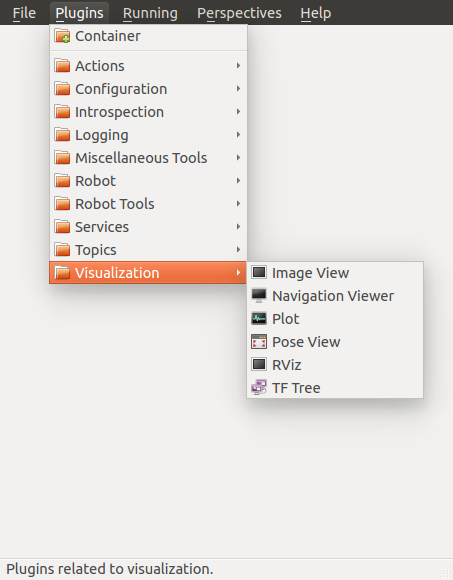
\includegraphics[width=0.8\columnwidth]{pictures/chapter6/rqt_plugin.png}
\caption{rqt 플러그인}
\end{figure}

\vspace{\baselineskip}
\noindent
이 들의 모든 플러그인을 설명하기 어렵고, 이번 강좌에서는 가장 빈번히 사용되는 rqt\_bag, rqt\_graph, rqt\_plot 등 에대해서 알아보도록 하겠다.

%-------------------------------------------------------------------------------
\subsection{rqt\_plot}\index{rqt\_plot}

rqt\_plot 은 2차원 데이터 플롯 툴이다. 플롯이라하면 좌료를 그리다라는 의미이다. 즉, ROS 메시지를 받아서 이를 좌표에 뿌리게 되는 것을 의미한다. 예를들어 turtlesim 노드 pose 메시지의 x 좌표와  y좌표를 좌표에 표기해보도록 하자. 우선, turtlesim 패키지의 turtlesim\_node 을 구동하자.

\begin{lstlisting}[language=ros]
$ rosrun turtlesim turtlesim_node 
\end{lstlisting}

다음으로, rqt\_plot 을 아래의 조건으로 구동하여 좌표를 작성한다. (원래는 rqt 를 구동후에 Plot 플러그인을 불러와서 GUI환경에서 토픽을 설정하면 되야하지만, 현재 버전에서는 이상하게 구동하지 않는다. 그러므로 아래의 명령어로 대채하여 설명한다.)

\begin{lstlisting}[language=ros]
rqt_plot /turtle1/pose/
\end{lstlisting}

다음으로, turtlesim 패키지의 turtle\_teleop\_key 을 구동하여, 화면속의 거북이를 이리저리 움직여보자.

\begin{lstlisting}[language=ros]
$ rosrun turtlesim turtle_teleop_key
\end{lstlisting}

그러면 빨간색 선이 거북이의 x위치가 x 좌표, 파란선이 거북이의 y위치가 y좌표에 표시됨을 확인할 수 있을 것이다. 이와 같이 2차원 데이터의 좌표 표시에 매우 유용한 툴로 지금은 turtlesim 을 이용하였지만, 사용자가 개발한 노드의 2차원 데이터 표시에 매우 유용할 것이다. 특히, 센서값 표시에 적합하다.

\begin{figure}[h]
\centering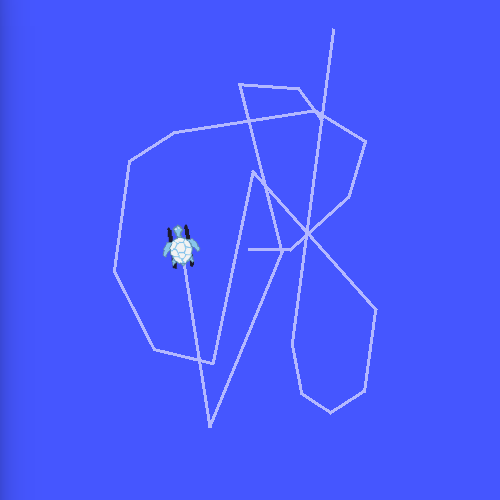
\includegraphics[height=50mm]{pictures/chapter6/turtlesim_rqt_plot1.png}
\centering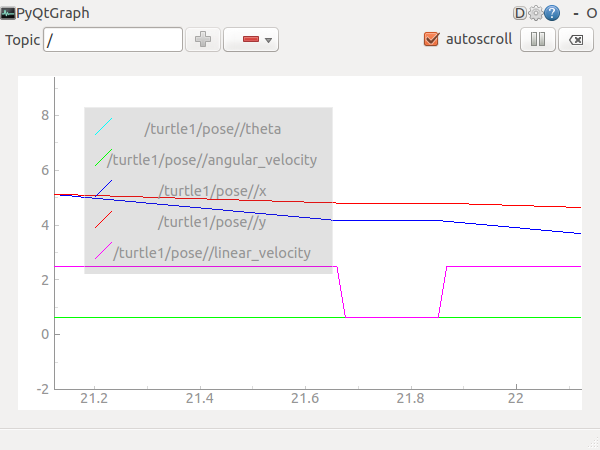
\includegraphics[height=50mm]{pictures/chapter6/turtlesim_rqt_plot2.png}
\caption{rqt\_plot 예제}
\end{figure}

%-------------------------------------------------------------------------------
\subsection{rqt\_bag}\index{rqt\_bag}

메시지 기록을 시각화한 GUI 툴이다. "로봇 운영체제 강좌 : ROS 정보 명령어 (rosbag)" 에서 다룬 내용을 시각화하면 편집 가능한 툴로 이미지 값등과 함께 편집할 때 매우 유용한 툴이다.

이를 테스트하기 위해서 위헤서 다룬 rqt\_graph 및 Image View 에서 다룬 turtlesim 및 uvc camera 관련의 노드들을 전부 실행해 주자. 그 뒤, 아래의 명령어로 카메라의 "/image\_raw" 와 터틀시뮬레이션의 "/turtle1/cmd\_vel" 값을 bag 파일로 생성하자.

\begin{lstlisting}[language=ros]
$ rosbag record /image_raw /turtle1/cmd_vel
\end{lstlisting}

그 후, 아래의 명령어로 rqt를 구동 후, 플러그인(Plugins) 메뉴에서 Bag를 선택한다. 그 뒤 왼쪽 상단의 폴더 모양(Load Bag)의 아이콘을 선택하여 방금전에 기록해둔 *.bag 파일을 불러오도록 하자. 그러면 아래의 화면처럼 영상 및 cmd\_vel 값을 확인할 수 있다. 또한, 이를 확대, 재생, 시간별 데이터 수 등을 확인할 수 있으며, 오른쪽 마우스를 누르면 Publish 라는 옵션이 있는데 이를 통해 메시지를 다시 발행할 수도 있다.

\begin{lstlisting}[language=ros]
$ rqt
\end{lstlisting}

\begin{figure}[h]
\centering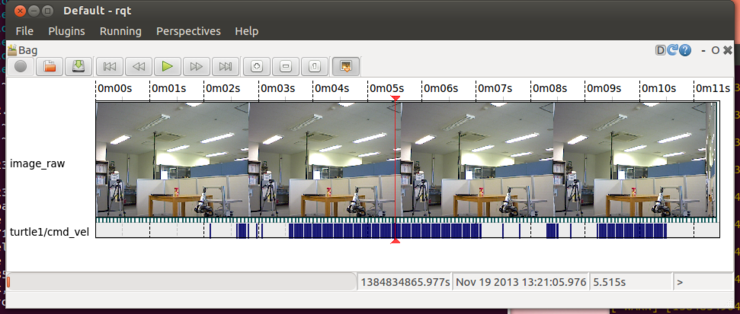
\includegraphics[width=0.9\columnwidth]{pictures/chapter6/rqt_bag.png}
\caption{rqtbag 예제}
\end{figure}

%-------------------------------------------------------------------------------
\subsection{rqt\_graph}\index{rqt\_graph}

현재 구동중인 노드 및 ROS 네트워크상에 전송되고 있는 메시지간의 상관 관계를 그래프로 나타내주는 툴이다. 현재 ROS 네트워크의 상황을 파악하는데에 매우 유용하다.

사용방법은 매우 간단한다. 아래의 명령어로 rqt를 구동후, 플러그인(Plugins) 메뉴에서 ROS Graph를 선택하면 그것으로 끝이다. 현재, 카메라 및 터틀봇시뮬레이션을 구동하셨을때의 노드 및 메시지의 상황은 아래 그림처럼 나타난다.

\begin{lstlisting}[language=ros]
$ rqt
\end{lstlisting}

\begin{figure}[h]
\centering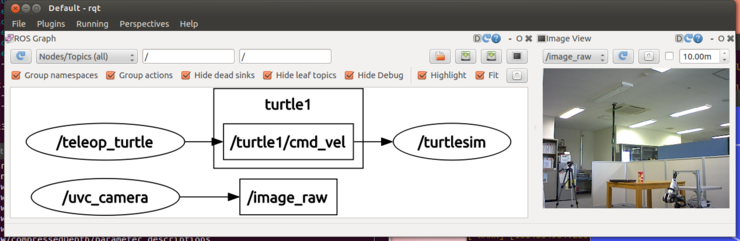
\includegraphics[width=0.9\columnwidth]{pictures/chapter6/rqt_graph.png}
\caption{rqt\_graph 예제}
\end{figure}

%-------------------------------------------------------------------------------
\subsection{Image View}\index{Image View}

카메라의 이미지 데이터를 표시하는 플러그인이다. 이미지 처리 프로세스는 아니지만, 단순히 영상을 확인하는 용도로는 매우 간단하기에 유용하다.

일반 USB CAM의 경우, UVC을 지원하기에 ROS의 "uvc\_camera"\footnote{ROS wiki, UVC Camera, http://wiki.ros.org/uvc\_camera} 패키지를 이용하면 된다. 우선, 아래의 명령어로 "uvc\_camera" 패키지를 설치하도록 하자.

\begin{lstlisting}[language=ROS]
$ sudo apt-get install ros-indigo-uvc-camera 
\end{lstlisting}

USB CAM을 컴퓨터의 USB에 연결하고, 아래의 명령어로 uvc\_camera 패키지의 uvc\_camera\_node 노드를 구동하자.

\begin{lstlisting}[language=ros]
$ rosrun uvc_camera uvc_camera_node
\end{lstlisting}

그 후, 아래의 명령어로 rqt를 구동후, 플러그인(Plugins) 메뉴에서 이미지 뷰(Image View)를 선택한다. 그 뒤 왼쪽 상단의 메시지 선택란을 "/image\_raw"를 선택하면 아래의 화면처럼 영상을 확인할 수 있다. 

\begin{lstlisting}[language=ros]
$ rqt
\end{lstlisting}

이상으로 rqt 를 대략적인 개요, 설치, 사용 방법에 대해서 설명하였다. 이 강좌를 통해서 모든 플러그인의 설명을 하는 것을 불가능했지만 위에서 설명한 몇가지 예를 기반으로 직접 사용해보기를 추천한다. ROS 노드와 같은 직접적으로 로봇 및 센서 처리에 관련한 내용은 아니지만, 이와 같은 작업들을 수행하는데 있어서 데이터를 저장, 보존, 수정, 현황파악 등에 도움이 되는 보조툴로서 사용가능하다. 













%-------------------------------------------------------------------------------
% -*- root: main.tex -*-
%-------------------------------------------------------------------------------
\chapterimage{chapter_head_7.pdf} 

%-------------------------------------------------------------------------------
\chapter{ROS 기본 프로그래밍}
\label{cha:RosPrograming}

%-------------------------------------------------------------------------------
\section{메시지, 토픽, 서비스, 매개변수}\index{메시지, 토픽, 서비스, 매개변수}

%-------------------------------------------------------------------------------
\subsection{ROS 메시지 통신}\index{ROS 메시지 통신}

이전 챕터 내용들이 ROS 개론을 설명하였다면 이번 부터가 본격적인 ROS 프로그래밍이라고 볼 수 있다. 이전 내용에서 제일 많이 나온 단어라고 치면 "메시지, 토픽, 서비스, 매개변수" 가 가장 빈번히 언급되었다. 그도 그럴것이, 메시지, 토픽, 서비스, 매개변수는 ROS 에서 가장 핵심 부분이라고 할 수 있다. 각기 목적에 따라 분화된 최소 실행 단위인 노드들은 메시지 통신을 통해 노드간의 입/출력 데이터를 주고 받는 처리를 하고 있다.

\begin{definition*}[메시지(message,msg)]
노드는 메시지를 통해 노드간의 데이터를 주고받게 된다. 메시지는 integer, floating point, boolean 와 같은 변수형태이다. 또한, 메시지안에 메시지를 품고 있는 간단한 데이터 구조 및 메시지들의 배열과 같은 구조도 사용할 수 있다. 

메세지를 이용한 통신방법으로는 TCPROS, UDPROS 방식등이 있으며, 단방향 메시지 송/수신 방식의 토픽과 양방향 메시지 요청/응답 방식의 서비스를 이용하고 있다.
\end{definition*}

메시지 통신을 하나의 그림으로 설명하면 아래와 같다고 볼 수 있다. 작은 목적 단위로 세분화된 실제 처리 프로그램인 노드는 다른 노드와의 데이터 송수신에 메시지 통신 방법을 이용하고 있다. 이 메시지 통신에는 크게 토픽과 서비스로 나뉘고 큰 틀에서는 매개변수 또한 메시지 통신이라고 볼 수있다. 이 세가지 메시지 통신방식인 토픽, 서비스, 매개변수를 이번 강좌에서 소개하고 각각의 특징을 ROS 프로그램 작성전에 미리 익혀두고자 한다. 그 후, 이어지는 강좌들에서 실전을 통해 자세히 다룰 예정이다.

\begin{figure}[h]
\centering\includegraphics[width=0.5\columnwidth]{pictures/chapter7/msgtrans1.png}
\caption{메시지 통신 상관 관계}
\end{figure}

%-------------------------------------------------------------------------------
\subsection{토픽 (topic)}\index{토픽 (topic)}

\begin{center} 
토픽(topic)은 \textbf{이야깃거리}이다.\\ 
\end{center}

발행자 노드가 하나의 이야깃거리에서 대해서 토픽이라는 이름으로 마스터에 등록한 후, 이야깃거리에 대한 이야기를 메시지 형태로 발행한다. 이 이야깃거리를 수신 받기를 원하는 구독자 노드는 마스터에 등록된 토픽의 이름에 해당되는 발행자 노드의 정보를 받는다. 이 정보를 기반으로 구독자 노드는 발행자 노드와 직접적으로 연결하여 메시지를 송/수신 받게 된다. \\

이를 나타낸 그림이 아래와 같다. 단방향 통신이기에 센서가 취득한 정보를 단순히 전달하는 용도로 많이 사용되는 메시지 통신 방식이다.

\begin{figure}[h]
\centering\includegraphics[width=0.7\columnwidth]{pictures/chapter7/msgtrans2.jpg}
\caption{토픽}
\end{figure}

%-------------------------------------------------------------------------------
\subsection{서비스(service)}\index{서비스(service)}

발행과 구독 개념의 토픽 통신 방식은 비동기 방식이라 필요에 따라서 주어진 데이터를 전송하고 받기에 매우 훌륭한 방법이다. 또한, 한번의 접속으로 지속적인 메시지를 송/수신하기 때문에 지속적으로 메시지를 발송해야하는 센서 데이터에 적합하여 많이 사용되고 있다. 

하지만, 경우에 따라서는 요청과 응답이 함께 사용되는 동기 방식의 메시지 교환 방식도 필요하다. 이에 따라, ROS에서는 서비스라는 이름으로 메시지 동기 방식을 제공하고 있다. 

서비스는 요청이 있을 경우에 응답을 하는 서비스 서버와 요청을 하고 응답을 받는 서비스 클라이언트로 나뉘어 있다. 서비스는 토픽과는 달리 1회성 메시지 통신이다. 서비스의 요청과 응답이 완료되면 연결된 두 노드의 접속은 끊기게 된다. 

이러한 서비스는 로봇에게 특정의 일을 수행하는 요청시에 명령어로써 많이 사용된다. 혹은, 특정 조건에 의해 이벤트를 발생해야할 노드에 사용되는 경우가 많다. 1회성 메시지 이기에 네트워크에 부하가 적다는 이유로 토픽을 대체하는 수단으로도 사용되는 등 매우 유용한 통신 수단이다.

\begin{figure}[h]
\centering\includegraphics[width=0.7\columnwidth]{pictures/chapter7/msgtrans3.png}
\caption{서비스}
\end{figure}

%-------------------------------------------------------------------------------
\subsection{매개변수(parameter)}\index{매개변수(parameter)}

노드에서 사용되는 매개변수를 말한다. 흔히, 윈도우즈 프로그램에서 *.ini 설정파일과 같다고 생각하면 된다. 디폴트로 설정 값들이 지정되어 있고, 필요에 의해서 외부에서 이 매개변수를 읽기, 쓰기가 가능하다. 특히, 상황에 맞추어 이 매개변수를 외부에서 쓰기기능을 이용하여 설정값을 실시간으로 바꿀수 있기에 매우 유용한 방법이다. 이는 엄밀히 따지면, 메시지 통신이라고 볼 수 없지만, 필자는 메시지를 이용한다는 점에서 메시지 통신의 범위에 속한다고 본다. 사용 예를 들자면 접속하는 USB포트 및 카메라 캘리브레이션 값, 속도 및 명령어들의 최대/최저 값 등의 설정 등을 꼽을 수 있다.

\begin{figure}[h]
\centering\includegraphics[width=0.6\columnwidth]{pictures/chapter7/msgtrans4.png}
\caption{매개변수}
\end{figure}

%-------------------------------------------------------------------------------
\section{메시지 발행자 노드와 구독자 노드 작성 및 실행}\index{메시지 발행자 노드와 구독자 노드 작성 및 실행}

%-------------------------------------------------------------------------------
\subsection{목적}

ROS 메시지 통신에서 사용되는 발행자(Publisher) 와 구독자(Subscriber) 라는 용어는 쉽게 우리말로 따지면 송신과 수신역할을 담당하게 된다. ROS에서는 송신측을 Publisher, 수신측을 Subscriber 라고 부르고 있다. 이 강좌에서는 간단한 메시지 파일을 작성해보고, 발행자(Publisher) 노드 와 구독자(Subscriber) 노드를 작성 및 실행하는 것을 목적으로 한다.

%-------------------------------------------------------------------------------
\subsection{패키지 생성}

아래의 명령어는 "oroca\_ros\_tutorials" 라는 패키지를 생성하는 명령어이다. 이 패키지는 의존하는 패키지로 "std\_msgs"와 "roscpp"를 옵션으로 달아주었다. ROS의 표준 메시지 패키지인 std\_msgs 와 ROS에서 c/c++을 사용하기 위하여 클라이언트라이브러인 roscpp를 사용하겠다는 것으로 패키지 생성에 앞어서 미리 설치해야한다는 의미이다. 이러한 의존하는 패키지의 설정은 패키지 생성할 때 지정할 수도 있지만, 생성 후 package.xml 에서 직접 입력하여도 된다.

\begin{lstlisting}[language=ROS]
$ cd ~/catkin_ws/src
$ catkin_create_pkg oroca_ros_tutorials std_msgs roscpp
\end{lstlisting}

위와 같이 패키지를 생성하였으면 "\textasciitilde/catkin\_ws/src"에 "oroca\_ros\_tutorials" 라는 패키지 폴더 및 ROS 패키지가 갖추어야할 기본 내부 폴더 및 CMakeLists.txt 와 package.xml가 생성된다. 다음은 아래와 같이 ls 명령어를 입력하여 내용을 보던가 윈도우의 탐색기와 같은 역할을 하는 GUI기반의 Nautilus를 이용하여 패키지 내부를 살펴보도록 하자.

\begin{lstlisting}[language=ROS]
$ ls
include       %*.......... 인클루드 폴더*)
src           %*.......... 소스코드 폴더*)
CMakeLists.txt%*.......... 빌드 설정 파일*)
\end{lstlisting}

%-------------------------------------------------------------------------------
\subsection{패키지 설정 파일 (package.xml) 수정}

ROS의 필수 설정 파일 중 하나인 package.xml 은 패키지 정보를 담은 XML 파일로써 패키지의 이름, 저작자, 라이선스, 의존성 패키지 등을 기술하고 있다. 아래의 명령어로 gedit 툴을 이용하여 파일을 열고 현재의 노드에 맞도록 수정해보자.

\begin{lstlisting}[language=ROS]
$ gedit package.xml 
\end{lstlisting}

아래의 코드는 package.xml 를 이번 노드에 맞도록 수정한 내용이다. 내용중에 필자의 개인 정보가 포함되어 있으니, 이를 자신에 맞게 수정해주길 바란다. 각 옵션의 세부 설명은 섹션~\ref{sec:RosBuildSystem}~\nameref{sec:RosBuildSystem}(pp.\pageref{sec:RosBuildSystem})를 참고하길 바란다.

\begin{lstlisting}[language=XML]
<?xml version="1.0"?>
<package>
  <name>oroca_ros_tutorials</name>
  <version>0.1.0</version>
  <description>The oroca_ros_tutorials package</description>

  <maintainer email="passionvirus@gmail.com">Yoonseok Pyo</maintainer>
  <url type="website">http://oroca.org</url>
  <url type="repository">https://github.com/oroca/oroca_ros_tutorials.git</url>
  <author email="passionvirus@gmail.com">Yoonseok Pyo</author>

  <license>MIT</license>

  <buildtool_depend>catkin</buildtool_depend>

  <build_depend>roscpp</build_depend>
  <build_depend>std_msgs</build_depend>
  <build_depend>message_generation</build_depend>

  <run_depend>roscpp</run_depend>
  <run_depend>std_msgs</run_depend>
  <run_depend>message_runtime</run_depend>

  <export>
  </export>
</package>
\end{lstlisting}

%-------------------------------------------------------------------------------
\subsection{빌드 설정 파일 (CMakeLists.txt) 수정}

ROS의 빌드 시스템인 캐킨(cakin)은 기본적으로 CMake를 이용하고 있어서 패키지 폴더에 CMakeLists.txt 라는 파일에 빌드 환경을 기술하고 있다. 이는 실행 파일 생성, 의존성 패키지 우선 빌드, 링크 생성 등을 설정하게 되어 있다.

\begin{lstlisting}[language=ROS]
$ gedit CMakeLists.txt 
\end{lstlisting}

아래의 코드는 CMakeLists.txt 를 이번 노드에 맞도록 수정한 내용이다.

\begin{lstlisting}[language=make]
cmake_minimum_required(VERSION 2.8.3)
project(oroca_ros_tutorials)

## Find catkin and any catkin packages
find_package(catkin REQUIRED COMPONENTS roscpp std_msgs message_generation)

## Declare ROS messages and services
add_message_files(FILES msgTutorial.msg)

## Generate added messages and services
generate_messages(DEPENDENCIES std_msgs)

## Declare a catkin package
catkin_package(
  #INCLUDE_DIRS include
  LIBRARIES oroca_ros_tutorials
  CATKIN_DEPENDS roscpp std_msgs
  DEPENDS system_lib
)

## Build node
include_directories(include ${catkin_INCLUDE_DIRS})

add_executable(ros_tutorial_msg_publisher src/ros_tutorial_msg_publisher.cpp)
target_link_libraries(ros_tutorial_msg_publisher ${catkin_LIBRARIES})
add_dependencies(ros_tutorial_msg_publisher oroca_ros_tutorials_generate_messages_cpp)

add_executable(ros_tutorial_msg_subscriber src/ros_tutorial_msg_subscriber.cpp)
target_link_libraries(ros_tutorial_msg_subscriber ${catkin_LIBRARIES})
add_dependencies(ros_tutorial_msg_subscriber oroca_ros_tutorials_generate_messages_cpp)
\end{lstlisting}

%-------------------------------------------------------------------------------
\subsection{메시지 파일 작성}

CMakeLists.txt 에 라는 파일에 "add\_message\_files(FILES msgTutorial.msg)" 라는 옵션을 넣었다. 이는 이번 노드에서 사용할 메시지인 msgTutorial.msg 를 빌드할때 포함하라는 이야기이다. 현재, msgTutorial.msg 는 생성하지 않았기에 아래와 같은 순서로 생성해주도록 하자.

\begin{lstlisting}[language=ROS]
$ cd ~/catkin_ws/src/oroca_ros_tutorials/     %*(패키지 폴더로 이동한다.)*)
$ mkdir msg               %*(패키지에 msg 라는 메시지 폴더를 신규 작성한다.)*)
$ cd msg                  %*(작성한 msg 폴더로 이동)*)
$ gedit msgTutorial.msg   %*(msgTutorial.msg 파일 신규 작성 및 내용 수정)*)
\end{lstlisting}

\noindent
내용으로는 아래와 같이 int32 메시지 형식에 data라는 이름의 메시지를 만들어주자.

\begin{lstlisting}[language=ROS]
int32 data
\end{lstlisting}

%-------------------------------------------------------------------------------
\subsection{발행자 노드 작성}

\begin{lstlisting}[language=make]
add_executable(ros_tutorial_msg_publisher src/ros_tutorial_msg_publisher.cpp)
\end{lstlisting}

CMakeLists.txt 에 위와 같은 실행 파일을 생성하는 옵션을 주었다. 즉, "ros\_tutorial\_msg\_publisher.cpp"라는 파일을 빌드하여 "ros\_tutorial\_msg\_publisher"라는 실행 파일을 만들라는 이야기이다. 아래의 순서대로 발행자 노드 기능을 수행하는 "ros\_tutorial\_msg\_publisher.cpp" 소스를 작성해 보자. 

\begin{lstlisting}[language=ROS]
$ cd ~/catkin_ws/src/oroca_ros_tutorials/ %*(패키지 폴더로 이동한다.)*)
$ cd src                                  %*(노드의 소스코드 폴더인 src 폴더로 이동)*)
$ gedit ros_tutorial_msg_publisher.cpp    %*(소스 파일 신규 작성 및 내용 수정)*)
\end{lstlisting}

\begin{lstlisting}[language=C++]
#include "ros/ros.h"                         //%* ROS 기본 헤더파일*)
#include "oroca_ros_tutorials/msgTutorial.h" //%* msgTutorial 메시지 파일헤더*)

int main(int argc, char **argv)              //%* 노드 메인 함수*)
{
  ros::init(argc, argv, "ros_tutorial_msg_publisher");  //%* 노드명 초기화*)
  ros::NodeHandle nh;                                   //%* 노드 핸들 선언*)

  //%* 발행자 선언, oroca\_ros\_tutorials 패키지의 msgTutorial 메시지 파일을 이용한*)
  //%* 발행자 ros\_tutorial\_pub 를 작성한다. 토픽명은 "ros\_tutorial\_msg" 이며,*)
  //%* 발행자 큐(queue) 사이즈를 100개로 설정한다는 것이다*)
  ros::Publisher ros_tutorial_pub = nh.advertise<oroca_ros_tutorials::msgTutorial>("ros_tutorial_msg", 100);

  //%* 루프 주기를 설정한다. "10" 이라는 것은 10Hz를 말하는 것으로 0.1초 간격으로 반복된다*)
  ros::Rate loop_rate(10); 

  int count = 0;    //%* 메시지에 사용될 변수 선언*)

  while (ros::ok())
  {
    oroca_ros_tutorials::msgTutorial msg; //%* msgTutorial 형식으로 msg 메시지를 선언*)
    msg.data = count;                 //%* count 변수를 이용하여 메시지 값을 정한다*)

    ROS_INFO("send msg = %d", count); //%* ROS\_INFO 함수를 이용하여 count 변수 표시*)

    ros_tutorial_pub.publish(msg);    //%* 메시지를 발행한다. 약 0.1초 간격으로 발행된다*)

    loop_rate.sleep();                //%* 위에서 정한 루프 주기에 따라 슬립에 들어간다*)

    ++count;                          //%* count 변수 1씩 증가*)
  }

  return 0;
}
\end{lstlisting}

%-------------------------------------------------------------------------------
\subsection{구독자 노드 작성}

\begin{lstlisting}[language=make]
add_executable(ros_tutorial_msg_subscriber src/ros_tutorial_msg_subscriber.cpp)
\end{lstlisting}

CMakeLists.txt 에 위와 같은 실행 파일을 생성하는 옵션을 주었다. 즉, "ros\_tutorial\_msg\_subscriber.cpp"라는 파일을 빌드하여 "ros\_tutorial\_msg\_subscriber"라는 실행 파일을 만들라는 이야기이다. 아래의 순서대로 구독자 노드 기능을 수행하는 "ros\_tutorial\_msg\_subscriber.cpp" 소스를 작성해 보자. 

\begin{lstlisting}[language=ROS]
$ cd ~/catkin_ws/src/oroca_ros_tutorials/ %*(패키지 폴더로 이동한다.)*)
$ cd src                                  %*(노드의 소스코드 폴더인 src 폴더로 이동)*)
$ gedit ros_tutorial_msg_subscriber.cpp   %*(소스 파일 신규 작성 및 내용 수정)*)
\end{lstlisting}

\begin{lstlisting}[language=C++]
#include "ros/ros.h"                         //%* ROS 기본 헤더파일*) 
#include "oroca_ros_tutorials/msgTutorial.h" //%* msgTutorial 메시지 파일 헤더*)

//%* 메시지 콜백함수로써, 밑에서 설정한 ros\_tutorial\_sub 구독자에 해당되는 메시지를*)
//%* 수신하였을때 동작하는 함수이다*)
//%* 입력 메시지로는 oroca\_ros\_tutorial 패키지의 msgTutorial 메시지를 받도록 되어있다 *)
void msgCallback(const oroca_ros_tutorials::msgTutorial::ConstPtr& msg)
{
  ROS_INFO("recieve msg: %d", msg->data);   //%* 수신된 메시지를 표시하는 함수*)
}

int main(int argc, char **argv)                         //%* 노드 메인 함수*)
{
  ros::init(argc, argv, "ros_tutorial_msg_subscriber"); //%* 노드명 초기화*)

  ros::NodeHandle nh;                                   //%* 노드 핸들 선언*)

  //%* 구독자 선언, oroca\_ros\_tutorials 패키지의 msgTutorial 메시지 파일을 이용한*)
  //%* 구독자 ros\_tutorial\_sub 를 작성한다. 토픽명은 "ros\_tutorial\_msg" 이며,*)
  //%* 구독자 큐(queue) 사이즈를 10개로 설정한다는 것이다*)
  ros::Subscriber ros_tutorial_sub = nh.subscribe("ros_tutorial_msg", 10, msgCallback);

  //%* 콜백함수 호출을 위한 함수로써, 메시지가 수신되기를 대기, 수신되었을 경우 콜백함수를 실행한다*)
  ros::spin();

  return 0;
}
\end{lstlisting}

%-------------------------------------------------------------------------------
\subsection{ROS 노드 빌드}

\begin{lstlisting}[language=ROS]
$ cd ~/catkin_ws  %*(catkin 폴더로 이동)*)
$ catkin_make     %*(catkin 빌드 실행)*)
\end{lstlisting}

위의 명령어로 oroca\_ros\_tutorials 패키지의 메지시 파일, 발행자 노드, 구독자 노드가 빌드되었다. 
oroca\_ros\_tutorials 패키지의 소스는 \textasciitilde/catkin\_ws/src/oroca\_ros\_tutorials/src 에 존재하고,oroca\_ros\_tutorials 패키지의 메시지 파일은 \textasciitilde/catkin\_ws/src/oroca\_ros\_tutorials/msg 에 존재한다.

이를 기반으로 빌드된 결과물은 ~/catkin\_ws 의 /build 및 /devel 에 각각 생성된다.
/build 에는 캐킨 빌드에서 사용된 설정 내용이 저장되며, /devel/lib/oroca\_ros\_tutorials 에는 실행 파일이, /devel/include/oroca\_ros\_tutorials 에는 메시지 파일로부터 자동 생성된 메시지 헤더파일이 저장된다. 각 생성 결과물이 궁금하다면 이 경로에 생성된 결과물을 확인해 보자.

%-------------------------------------------------------------------------------
\subsection{발행자 실행}

※ 주의! 노드 실행에 앞서서 roscore를 실행해주는 것을 잊지 말자!

\begin{lstlisting}[language=ROS]
$ rosrun oroca_ros_tutorials ros_tutorial_msg_publisher
\end{lstlisting}

ROS 노드 실행 명령어인 rosrun 을 이용하여, oroca\_ros\_tutorials 패키지의 ros\_tutorial\_msg\_publisher 노드를 구동하라는 명령어이다. 이를 실행하게 되면 아래와 같은 출력 화면을 볼 수 있다. 내부에 선언된 count 값이 표시되고 있으며, ROS 메시지로 발부되고 있다. 

\begin{figure}[h]
\centering\includegraphics[width=0.8\columnwidth]{pictures/chapter7/rosrun_ros_tutorial_msg_publisher.png}
\caption{ros\_tutorial\_msg\_publisher 노드 실행시의 화면}
\end{figure}

이전에 익힌 rostopic 명령어를 이용하여 현재 ROS 네트워크에서 사용중인 토픽의 목록을 확인해보고, 위에서 실행한 발행자 노드에서 발행중인 메시지를 확인해보도록 하자.

\vspace{\baselineskip}
\begin{lstlisting}[language=ROS]
$ rostopic list
/ros_tutorial_msg
/rosout
/rosout_agg
$ rostopic echo /ros_tutorial_msg
\end{lstlisting}

rostopic list 라는 옵션을 붙인 명령어로 ros\_tutorial\_msg 토픽이 있음을 확인하였다. rostopic echo /ros\_tutorial\_msg 이라는 명령어로 ros\_tutorial\_msg 토픽의 메시지를 확인해보자. 아래와 같이 실시간으로 발행되는 메시지를 확인할 수 있을 것이다.

\begin{figure}[h]
\centering\includegraphics[width=0.8\columnwidth]{pictures/chapter7/rostopic_echo.png}
\caption{ros\_tutorial\_msg 토픽의 수신된 내역}
\end{figure}

\newpage
%-------------------------------------------------------------------------------
\subsection{구독자 실행}

\begin{lstlisting}[language=ROS]
$ rosrun oroca_ros_tutorials ros_tutorial_msg_subscriber 
\end{lstlisting}

ROS 노드 실행 명령어인 rosrun 을 이용하여, oroca\_ros\_tutorials 패키지의 ros\_tutorial\_msg\_subscriber  노드를 구동하라는 명령어이다. 이를 실행하게 되면 아래와 같은 출력 화면을 볼 수 있다. 발행자에서 발행된 ros\_tutorial\_msg 토픽의 메시지를 수신받아 값이 표시되고 있다.

\begin{figure}[h]
\centering\includegraphics[width=0.8\columnwidth]{pictures/chapter7/rosrun_ros_tutorial_msg_subscriber.png}
\caption{ros\_tutorial\_msg\_subscriber 노드 실행시의 화면}
\end{figure}

\newpage
%-------------------------------------------------------------------------------
\subsection{실행된 노드들의 통신 상태 확인}

\begin{lstlisting}[language=ROS]
$ rqt_graph
\end{lstlisting}

\begin{lstlisting}[language=ROS]
$ rqt
\end{lstlisting}

위 두 명령어 중 하나를 사용하여 rqt 를 실행 후, 플러그인(plugins)에서 ROS Graph 를 선택하면 아래의 그림처럼 현재 ROS 에서 구동중인 노드 및 메시지를 확인할 수 있다. 현재 ROS 네트워크상에는, 구독자 노드 (ros\_tutorial\_msg\_publisher) 에서 발행한 토픽 (ros\_tutorial\_msg) 이 발행중이고 이를 구독자 노드 (ros\_tutorial\_msg\_subscriber) 에서 수신하고 있음을 확인할 수 있다.

\begin{figure}[h]
\centering\includegraphics[width=0.7\columnwidth]{pictures/chapter7/rqt_graph_oroca_ros_tutorials.png}
\caption{rqt\_graph를 통해서 본 두 노드의 관계도}
\end{figure}

%-------------------------------------------------------------------------------
\section{서비스 서버 노드와 클라이언트 노드 작성 및 실행}\index{서비스 서버 노드와 클라이언트 노드 작성 및 실행}

%-------------------------------------------------------------------------------
\subsection{서비스의 목적}

서비스는 요청이 있을 경우에 응답을 하는 서비스 서버와 요청을 하고 응답을 받는 서비스 클라이언트로 나뉘어 있다. 서비스는 토픽과는 달리 1회성 메시지 통신이다. 서비스의 요청과 응답이 완료되면 연결된 두 노드의 접속은 끊기게 된다.이러한 서비스는 로봇에게 특정의 일을 수행하는 요청시에 명령어로써 많이 사용된다. 혹은, 특정 조건에 의해 이벤트를 발생해야할 노드에 사용되는 경우가 많다. 1회성 메시지 이기에 네트워크에 부하가 적다는 이유로 토픽을 대체하는 수단으로도 사용되는 등 매우 유용한 통신 수단이다.

이 강좌에서는 간단한 서비스 파일 작성해보고 서비스 서버(server) 노드 와 서비스 클라이언트(client) 노드를 작성 및 실행하는 것을 목적으로 한다.

%-------------------------------------------------------------------------------
\subsection{패키지 생성}

이전 강좌에서 oroca\_ros\_tutorials 라는 패키지를 생성하는 설명을 하였다. 위 강좌를 참조하기 바라고, 위 강좌에서 이미 패키지를 생성한 것으로 보고 패키지 생성은 건너 뛰도록 하자.

%-------------------------------------------------------------------------------
\subsection{패키지 설정 파일 (package.xml) 수정}

이번 강좌에서는 패키지 정보를 담은 package.xml 를 수정할 부분이 없다.

%-------------------------------------------------------------------------------
\subsection{빌드 설정 파일 (CMakeLists.txt) 수정}

ROS의 빌드 시스템인 캐킨(cakin)은 기본적으로 CMake를 이용하고 있어서 패키지 폴더에 CMakeLists.txt 라는 파일에 빌드 환경을 기술하고 있다. 이는 실행 파일 생성, 의존성 패키지 우선 빌드, 링크 생성 등을 설정하게 되어 있다.

\begin{lstlisting}[language=ROS]
$ gedit CMakeLists.txt 
\end{lstlisting}

아래의 코드는 CMakeLists.txt 를 이번 노드에 맞도록 수정한 내용이다. 이전 메시지 발행자 노드와 구독자 노드 작성에 서비스 파일을 새로 추가하고, 서비스 서버 노드와 클라이언트 노드에 대한 내용을 추가하였다. 각 옵션의 세부 설명은 섹션~\ref{sec:RosBuildSystem}~\nameref{sec:RosBuildSystem}(pp.\pageref{sec:RosBuildSystem})를 참고하길 바란다.

\begin{lstlisting}[language=make]
cmake_minimum_required(VERSION 2.8.3)
project(oroca_ros_tutorials)

## Find catkin and any catkin packages
find_package(catkin REQUIRED COMPONENTS roscpp std_msgs message_generation)

## Declare ROS messages and services
add_message_files(FILES msgTutorial.msg)
add_service_files(FILES srvTutorial.srv)

## Generate added messages and services
generate_messages(DEPENDENCIES std_msgs)

## Declare a catkin package
catkin_package(
  INCLUDE_DIRS include
  LIBRARIES oroca_ros_tutorials
  CATKIN_DEPENDS roscpp std_msgs
  DEPENDS system_lib
)

## Build node
include_directories(include ${catkin_INCLUDE_DIRS})

add_executable(ros_tutorial_msg_publisher src/ros_tutorial_msg_publisher.cpp)
target_link_libraries(ros_tutorial_msg_publisher ${catkin_LIBRARIES})
add_dependencies(ros_tutorial_msg_publisher oroca_ros_tutorials_generate_messages_cpp)

add_executable(ros_tutorial_msg_subscriber src/ros_tutorial_msg_subscriber.cpp)
target_link_libraries(ros_tutorial_msg_subscriber ${catkin_LIBRARIES})
add_dependencies(ros_tutorial_msg_subscriber oroca_ros_tutorials_generate_messages_cpp)

add_executable(ros_tutorial_srv_server src/ros_tutorial_srv_server.cpp)
target_link_libraries(ros_tutorial_srv_server ${catkin_LIBRARIES})
add_dependencies(ros_tutorial_srv_server oroca_ros_tutorials_generate_messages_cpp)

add_executable(ros_tutorial_srv_client src/ros_tutorial_srv_client.cpp)
target_link_libraries(ros_tutorial_srv_client ${catkin_LIBRARIES})
add_dependencies(ros_tutorial_srv_client oroca_ros_tutorials_generate_messages_cpp)
\end{lstlisting}

%-------------------------------------------------------------------------------
\subsection{서비스 파일 작성}

CMakeLists.txt 에 라는 파일에 "add\_service\_files(FILES srvTutorial.srv)" 라는 옵션을 넣었다. 이는 이번 노드에서 사용할 서비스인 srvTutorial.srv 를 빌드할 때 포함하라는 이야기이다. 현재, srvTutorial.srv 는 생성하지 않았기에 아래와 같은 순서로 생성해주도록 하자.

\begin{lstlisting}[language=ROS]
$ roscd oroca_ros_tutorials %*(패키지 폴더로 이동한다.*)
$ mkdir srv                 %*(패키지에 srv 라는 서비스 폴더를 신규 작성한다.*)
$ cd srv                    %*(작성한 srv 폴더로 이동*)
$ gedit srvTutorial.srv     %*(srvTutorial.srv 파일 신규 작성 및 내용 수정*)
\end{lstlisting}

\noindent
내용으로는 아래와 같이 int64 형식의 a, b라는 서비스 요청(request)과, sum 라는 이라는 서비스 응답(response)을 만들어주자. "---" 는 요청과 응답을 구분시켜주는 구분자이다.

\begin{lstlisting}[language=ROS]
int64 a
int64 b
---
int64 result
\end{lstlisting}

%-------------------------------------------------------------------------------
\subsection{서비스 서버 노드 작성}

\begin{lstlisting}[language=make]
add_executable(ros_tutorial_srv_server src/ros_tutorial_srv_server.cpp)
\end{lstlisting}

CMakeLists.txt 에 위와 같은 실행 파일을 생성하는 옵션을 주었다. 즉, "ros\_tutorial\_srv\_server.cpp"라는 파일을 빌드하여 "ros\_tutorial\_srv\_server"라는 실행 파일을 만들라는 이야기이다. 아래의 순서대로 서비스 서버 노드 기능을 수행하는 "ros\_tutorial\_srv\_server.cpp" 소스를 작성해 보자. 

\begin{lstlisting}[language=ROS]
$ roscd oroca_ros_tutorials         %*(패키지 폴더로 이동한다.*)
$ cd src                            %*(노드의 소스코드 폴더인 src 폴더로 이동*)
$ gedit ros_tutorial_srv_server.cpp %*(소스 파일 신규 작성 및 내용 수정*)
\end{lstlisting}

\begin{lstlisting}[language=C++]
#include "ros/ros.h"                         //%* ROS 기본 헤더파일*)
#include "oroca_ros_tutorials/srvTutorial.h" //%* srvTutorial 서비스 파일 헤더*)

//%* 서비스 요청이 있을 경우, 아래의 처리를 수행한다*)
//%* 서비스 요청은 res, 서비스 응답은 req로 설정하였다*)
bool calculation(oroca_ros_tutorials::srvTutorial::Request  &req,
         oroca_ros_tutorials::srvTutorial::Response &res)
{
  //%* 서비스 요청시 받은 a와 b 값을 더하여 서비스 응답값에 저장한다*)
  res.result = req.a + req.b;  

  //%* 서비스 요청에 사용된 a, b값의 표시 및 서비스 응답에 해당되는 result 값을 출력한다*)
  ROS_INFO("request: x=%ld, y=%ld", (long int)req.a, (long int)req.b);
  ROS_INFO("sending back response: [%ld]", (long int)res.result);

  return true;
}

int main(int argc, char **argv)                     //%* 노드 메인 함수*)
{
  ros::init(argc, argv, "ros_tutorial_srv_server"); //%* 노드명 초기화*)
  ros::NodeHandle nh;                               //%* 노드 핸들 선언*)

  //%* 서비스 서버 선언, oroca\_ros\_tutorials 패키지의 srvTutorial 서비스 파일을 이용한*)
  //%* 서비스 서버 ros\_tutorial\_service\_server 를 작성한다. 서비스명은 "ros\_tutorial\_srv" 이며,*)
  //%* 서비스 요청이 있을경우, calculation 라는 함수를 실행하라는 설정이다*)
  ros::ServiceServer ros_tutorial_service_server = nh.advertiseService("ros_tutorial_srv", calculation);

  ROS_INFO("ready srv server!");

  ros::spin();  //%* 서비스 요청을 대기한다*)

  return 0;
}
\end{lstlisting}

%-------------------------------------------------------------------------------
\subsection{서비스 클라이언트 노드 작성}

\begin{lstlisting}[language=make]
add_executable(ros_tutorial_srv_client src/ros_tutorial_srv_client.cpp)
\end{lstlisting}

CMakeLists.txt 에 위와 같은 실행 파일을 생성하는 옵션을 주었다. 즉, "ros\_tutorial\_srv\_client.cpp"라는 파일을 빌드하여 "ros\_tutorial\_srv\_client"라는 실행 파일을 만들라는 이야기이다. 아래의 순서대로 서비스 클라이언트 노드 기능을 수행하는 "ros\_tutorial\_srv\_client.cpp" 소스를 작성해 보자. 

\begin{lstlisting}[language=ROS]
$ cd ~/catkin_ws/src/oroca_ros_tutorials/ %*(패키지 폴더로 이동한다.)*)
$ cd src                                  %*(노드의 소스코드 폴더인 src 폴더로 이동)*)
$ gedit ros_tutorial_srv_client.cpp       %*(소스 파일 신규 작성 및 내용 수정)*)
\end{lstlisting}

\begin{lstlisting}[language=C++]
//%* ROS 기본 헤더파일*)
#include "ros/ros.h"
//%* srvTutorial 서비스 파일 헤더*)
#include "oroca_ros_tutorials/srvTutorial.h"
//%* atoll 함수 사용을 위한 라이브러리*)
#include <cstdlib>

//%* 노드 메인 함수*)
int main(int argc, char **argv)
{
  //%* 노드명 초기화*)
  ros::init(argc, argv, "ros_tutorial_srv_client");

  //%* 입력값 오류 처리*)
  if (argc != 3)                                    
  {
    ROS_INFO("cmd : rosrun ros_tutorial ros_tutorial_service_client arg0 arg1");
    ROS_INFO("arg0: double number, arg1: double number");
    return 1;
  }

  //%* ROS 시스템과 통신을 위한 노드 핸들 선언*)
  ros::NodeHandle nh;

  //%* 서비스 클라이언트 선언, oroca\_ros\_tutorials 패키지의 srvTutorial 서비스 파일을 이용한*)
  //%* 서비스 클라이언트 ros\_tutorial\_service\_client 를 작성한다.*)
  //%* 서비스명은 "ros\_tutorial\_srv" 이다*)
  ros::ServiceClient ros_tutorial_service_client = nh.serviceClient<oroca_ros_tutorials::srvTutorial>("ros_tutorial_srv");

  //%* srv 라는 이름으로 srvTutorial 서비스 파일을 이용하는 서비스 파일을 선언한다*)
  oroca_ros_tutorials::srvTutorial srv;

  //%* 서비스 요청 값으로 노드가 실행될 때 입력으로 사용된 매개변수를 각각의 a, b에 저장한다*)
  srv.request.a = atoll(argv[1]);
  srv.request.b = atoll(argv[2]);

  //%* 서비스를 요청하고, 요청이 받아들여 졌을 경우, 응답값을 표시한다*)
  if (ros_tutorial_service_client.call(srv))
  {
    ROS_INFO("send srv, srv.Request.a and b: %ld, %ld", (long int)srv.request.a, (long int)srv.request.b);
    ROS_INFO("recieve srv, srv.Response.result: %ld", (long int)srv.response.result);
  }
  else
  {
    ROS_ERROR("Failed to call service ros_tutorial_srv");
    return 1;
  }

  return 0;
}
\end{lstlisting}

%-------------------------------------------------------------------------------
\subsection{ROS 노드 빌드}

\begin{lstlisting}[language=ROS]
$ cd ~/catkin_ws && catkin_make %*(catkin 폴더로 이동 후 catkin 빌드 실행)*)
\end{lstlisting}

위의 명령어로 oroca\_ros\_tutorials 패키지의 서비스 파일, 서비스 서버 노드 및 클라이언트 노드가 빌드되었다. oroca\_ros\_tutorials 패키지의 소스는 \textasciitilde/catkin\_ws/src/oroca\_ros\_tutorials/src 에 존재하고, oroca\_ros\_tutorials 패키지의 서비스 파일은 \textasciitilde/catkin\_ws/src/oroca\_ros\_tutorials/srv 에 존재한다.

이를 기반으로 빌드된 결과물은 \textasciitilde/catkin\_ws/build 및 \textasciitilde/catkin\_ws/devel 에 각각 생성된다. \textasciitilde/catkin\_ws/build 에는 캐킨 빌드에서 사용된 설정 내용이 저장되며, \textasciitilde/catkin\_ws/devel/lib/oroca\_ros\_tutorials 에는 실행 파일이, \textasciitilde/catkin\_ws/devel/include/oroca\_ros\_tutorials 에는 메시지 파일로부터 자동 생성된 서비스 헤더파일이 저장된다. 각 생성 결과물이 궁금하다면 이 경로에 생성된 결과물을 확인해 보자.

%-------------------------------------------------------------------------------
\subsection{서비스 서버 실행}

※ 주의! 노드 실행에 앞서서 roscore를 실행해주는 것을 잊지 말자!

\begin{lstlisting}[language=ROS]
$ rosrun oroca_ros_tutorials ros_tutorial_srv_server 
[ INFO] [1385278089.933322980]: ready srv server!
\end{lstlisting}

위에서 작성해본 서비스 서버는 서비스 요청이 있기전까지 아무런 처리를 하지않고 기다리도록 프로그래밍 하였다. 그러므로 위 명령어를 실행하면 서비스 서버는 서비스 요청 대기를 하게 된다.

%-------------------------------------------------------------------------------
\subsection{서비스 클라이언트 실행}

\begin{lstlisting}[language=ROS]
$ rosrun oroca_ros_tutorials ros_tutorial_srv_client 2 3
[ INFO] [1385278213.278198846]: send srv, srv.Request.a and b: 2, 3
[ INFO] [1385278213.278348033]: recieve srv, srv.Response.result: 5
\end{lstlisting}

위와 같이 서비스 클라이언트를 실행하면서 입력해준 실행 매개변수에 2와 3을 서비스 요청 값으로 전송하도록 프로그램밍 하였다. 그 결과, 2와 3은 각각 서비스 요청의 a, b 값으로 서비스 요청을 하게되고, 그 결과값으로 그 둘의 합인 5를 전송받았다. 이 강좌에서는 단순하게 실행 매개변수로 이를 이용하였으나, 실제 활용에 있어서는 명령어로 대체해도 되고, 계산되어야할 값, 트리거용 변수 등을 서비스 요청 값으로 사용할 수도 있다.

\begin{figure}[h]
\centering\includegraphics[width=\columnwidth]{pictures/chapter7/rqt_graph_oroca_ros_tutorials.png}
\caption{왼쪽: 서비스 서버 / 오른쪽: 서비스 클라이언트}
\end{figure}

※ 참고로, 서비스는 토픽과는 달리, 1회성이기에 ROS Graph 등에서 확인할 수 없다.

%-------------------------------------------------------------------------------
\subsection{서비스 콜 명령어 사용하는 방법 (rosservice call)}

서비스를 요청하는 방법으로는 위 9번 처럼 서비스 클라이언트 노드를 실행하는 방법도 있지만 "rosservice call" 이라는 명령어 및 rqt의 ServiceCaller 를 이용하는 방법이 있다. 그 중 우선, "rosservice call" 를 사용하는 방법에 대해서 알아보자.

\begin{lstlisting}[language=ROS]
$ rosservice call /ros_tutorial_srv 3 4
result: 7
\end{lstlisting}

위 처럼 "rosservice call" 명령어 뒤에 "/ros\_tutorial\_srv" 처럼 해당하는 서비스명을 적어주고 그 뒤를 이어 서비스 요청에 필요한 매개변수를 적어주면 된다. 위 예제에서는 아래와 같이 요청으로 int64 형태의 a 와 b 를 설정해 두었기때문에 매개변수로 "3"과 "4"를 입력해주었다. 이에 대한 서비스 응답의 결과값은 int64 형태의 sum이 7 이라고 돌아왔음을 확인 할 수 있다.  

\begin{lstlisting}[language=ROS]
int64 a
int64 b
---
int64 result
\end{lstlisting}

%-------------------------------------------------------------------------------
\subsection{GUI 툴인 ServiceCaller 를 사용하는 방법 (RQT ServiceCaller)}

마직막으로 gui 형태의 인터페이스를 이용한 rqt의 ServiceCaller 를 이용하는 방법이 있다. 우선, ROS의 GUI 툴인 rqt를 실행하자. 명령어는 아래와 같다.

\begin{lstlisting}[language=ROS]
$ rqt
\end{lstlisting}

그 뒤, 프로그램의 위 메뉴 중에 플러그인(Plugins)에서 ServiceCaller 를 선택하면 아래와 같은 화면이 나온다. 여기서 상단의 Service 에서 서비스명을 선택해주면 Request 에 서비스요청에 필요한 정보가 보인다. 서비스 요청을 해주기 위해서는 각 요청 정보의 Expressin에 정보를 기입해주면 된다. 필자는 a 란에 10, b란에 5를 입력하였다. 그 뒤, 오른쪽 상단의 녹색 전화기 모양의 Call 아이콘을 클릭해주면 서비스 요청이 실행되고, 화면 하단에 Response 란에 서비스 응답에 대한 결과가 표시된다. 위 10번에서 설명한 rosservice call 은 터미널에서 바로 실행이라는 장점이 있지만 리눅스 및 ROS 명령어 사용에 익숙하지 않은 사람에게는 ServiceCaller 를 추천한다.

\begin{figure}[h]
\centering\includegraphics[width=0.7\columnwidth]{pictures/chapter7/rqt_service_caller.png}
\caption{ServiceCaller rqt플러그인을 통한 서비스 요청}
\end{figure}

관련 소스는 https://github.com/oroca/oroca\_ros\_tutorials 에서 확인해 볼 수 있다. 바로 적용해 보고 싶은 경우는 아래와 같이 catkin\_ws/src 에서 아래의 명령어를 실행해주면 된다.

\begin{lstlisting}[language=ROS]
$ cd ~/catkin_ws/src      %*(catkin/src 폴더로 이동*)
$ git clone https://github.com/oroca/oroca_ros_tutorials.git
$ cd ~/catkin_ws          %*(catkin 폴더로 이동*)
$ catkin_make             %*(catkin 빌드 실행*)
\end{lstlisting}

\newpage
%-------------------------------------------------------------------------------
\section{매개변수 사용법}\index{매개변수 사용법}

%-------------------------------------------------------------------------------
\subsection{매개변수(parameter)}

\begin{definition*}[매개변수(parameter)]\label{def:RosParameter}
노드에서 사용되는 매개변수를 말한다. 흔히, 윈도우즈 프로그램에서 *.ini 설정파일과 같다고 생각하면 된다. 디폴트로 설정 값들이 지정되어 있고, 필요에 의해서 외부에서 이 매개변수를 읽기, 쓰기가 가능하다. 특히, 상황에 맞추어 이 매개변수를 외부에서 쓰기기능을 이용하여 설정값을 실시간으로 바꿀수 있기에 매우 유용한 방법이다. 예를들어 접속하는 USB포트 및 카메라 캘리브레이션 값, 속도 및 명령어들의 최대/최저 값 등의 설정등을 지정할 수 있다.
\end{definition*}

위의 매개변수는 강좌에서 여러번 언급되었으나 이번 강좌에서 처음으로 실습까지 다룰 것이다. 매개변수 개념과 관련된 좀 더 자세한 내용에 대해서 아래의 링크의 강좌를 참조하도록 하자. 특히, rosparam 명령어는 아래의 강좌를 통해서 이해했다는 전제하에 강좌를 진행하도록 하겠다.

%-------------------------------------------------------------------------------
\subsection{매개변수를 활용한 노드 작성}

이번에서 이전 서비스 서버 노드와 클라이언트 노드에서 다룬 ros\_tutorial\_srv\_server.cpp 의 소스를 수정하여 서비스 요청으로 입력된 a 와 b 를 단순히 덧셈하는 것이 아니라, 사칙연산을 할 수있도록 매개변수를 활용해 볼 것이다. 아래의 순서대로 이전 강좌에서 작성해둔 ros\_tutorial\_srv\_server.cpp 소스를 수정하도록 하자.

\begin{lstlisting}[language=ROS]
$ roscd oroca_ros_tutorials         %*(패키지 폴더로 이동한다.*)
$ cd src                            %*(노드의 소스코드 폴더인 src 폴더로 이동*)
$ gedit ros_tutorial_srv_server.cpp %*(소스 파일 신규 작성 및 내용 수정*)
\end{lstlisting}

\begin{lstlisting}[language=C++]
#include "ros/ros.h"                         //%* ROS 기본 헤더파일*)
#include "oroca_ros_tutorials/srvTutorial.h" //%* srvTutorial 서비스 파일 헤더*)
 
#define PLUS           1    //%* 덧셈*)
#define MINUS          2    //%* 빼기*)
#define MULTIPLICATION 3    //%* 곱하기*)
#define DIVISION       4    //%* 나누기*)
 
int g_operator = PLUS;
 
//%* 서비스 요청이 있을 경우, 아래의 처리를 수행한다*)
//%* 서비스 요청은 res, 서비스 응답은 req로 설정하였다*)
bool calculation(oroca_ros_tutorials::srvTutorial::Request  &req,
                 oroca_ros_tutorials::srvTutorial::Response &res)
{
  //%* 서비스 요청시 받은 a와 b 값을 파라미터값에 따라 연산자를 달리한다.*)
  //%* 계산한 후 서비스 응답값에 저장한다*)
  switch(g_operator){
    case PLUS:
         res.result = req.a + req.b; break;
    case MINUS:
         res.result = req.a - req.b; break;
    case MULTIPLICATION:
         res.result = req.a * req.b; break;  
    case DIVISION:
         if(req.b == 0){
           res.result = 0; break;
         }  
         else{
           res.result = req.a / req.b; break;  
         }
    default:
         res.result = req.a + req.b; break;
  }
 
  //%* 서비스 요청에 사용된 a, b값의 표시 및 서비스 응답에 해당되는 result 값을 출력한다*)
  ROS_INFO("request: x=%ld, y=%ld", (long int)req.a, (long int)req.b);
  ROS_INFO("sending back response: [%ld]", (long int)res.result);
 
  return true;
}
 
int main(int argc, char **argv)                     //%* 노드 메인 함수*)
{
  ros::init(argc, argv, "ros_tutorial_srv_server"); //%* 노드명 초기화*)
 
  ros::NodeHandle nh;                       //%* 노드 핸들 선언*)
 
  nh.setParam("calculation_method", PLUS);  //%* 매개변수 초기설정*)
 
  //%* 서비스 서버 선언, oroca\_ros\_tutorials 패키지의 srvTutorial 서비스 파일을 이용한*)
  //%* 서비스 서버 ros\_tutorial\_service\_server 를 작성한다. 서비스명은 "ros\_tutorial\_srv" 이며,*)
  //%* 서비스 요청이 있을경우, calculation 라는 함수를 실행하라는 설정이다*)
  ros::ServiceServer ros_tutorial_service_server =
    nh.advertiseService("ros_tutorial_srv", calculation);
 
  ROS_INFO("ready srv server!");
   
  ros::Rate r(10); //%* 10 hz*)
 
  while (1)
  {
    //%* 연산자를 매개변수로부터 받은 값으로 변경한다*)
    nh.getParam("calculation_method", g_operator);  
    ros::spinOnce();  //%* 콜백함수 처리루틴*)
    r.sleep();        //%* 루틴 반복을 위한 sleep 처리*)
  }
 
  return 0;
}
\end{lstlisting}

\noindent
대부분은 이전 강좌에서 다룬 내용과 비슷하다. 이 중에서 매개변수 활용을 위해 추가된 부분에 대해서 알아보도록 하자. 특히, 49줄과 62줄에서 다룬 "setParam", "getParam" 가 매개변수 사용에서 제일 중요하다. 하지만, 매우 간단한 사용법이기때문에 함수 사용만 봐도 충분히 이해가 될 것이다.

%-------------------------------------------------------------------------------
\subsection{매개변수 설정}\index{매개변수 설정}

아래의 소스는 "calculation\_method" 라는 이름의 매개변수를 PLUS 라는 값으로 설정한다는 것이다. PLUS 는 위 소스에서 1 이므로 "calculation\_method" 매개변수는 1이 되고, 위 소스에서 서비스 요청으로 받은 값을 덧셈하여 서비스 응답을 하게 된다.

\begin{lstlisting}[language=C++]
nh.setParam("calculation_method", PLUS);
\end{lstlisting}

\noindent
참로고 매개변수는 integers, floats, boolean, string, dictionaries, list 등으로 설정할 수 있다. 간단히 예를 들자면, 1 은 integer, 1.0은 floats, internetofthings은 string, true는 boolean, [1,2,3]은 integers 의 list, {a: b, c: d}은 dictionary이다. 

%-------------------------------------------------------------------------------
\subsection{매개변수 읽기}\index{매개변수 읽기}

아래의 소스는 "calculation\_method" 라는 이름의 매개변수를 불러와서 g\_operator 의 값으로 설정한다는 것이다. 이에 따라서 위 소스에서의 g\_operator 는 매 0.1초마다 매개변수의 값을 확인하여 서비스 요청으로 받은 값을 사칙연사중 어떤 계산을 하여 처리할 지 결정하게 된다.

\begin{lstlisting}[language=C++]
nh.getParam("calculation_method", g_operator);
\end{lstlisting}

%-------------------------------------------------------------------------------
\subsection{노드 빌드 및 실행}\index{노드 빌드 및 실행}

\begin{lstlisting}[language=ROS]
$ cd ~/catkin_ws && catkin_make
\end{lstlisting}

\noindent
위의 명령어로 oroca\_ros\_tutorials 패키지의 서비스 서버 노드가 빌드되었다. 

\begin{lstlisting}[language=ROS]
$ rosrun oroca_ros_tutorials ros_tutorial_srv_server 
[ INFO] [1385278089.933322980]: ready srv server!
\end{lstlisting}

\noindent
위 명령어를 실행하면 서비스 서버는 서비스 요청 대기를 하게 된다.

%-------------------------------------------------------------------------------
\subsection{매개변수 리스트 보기}\index{매개변수 리스트 보기}

\begin{lstlisting}[language=ROS]
$ rosparam list
/calculation_method
/rosdistro
/roslaunch/uris/host_192_168_4_185__60432
/rosversion
/run_id
\end{lstlisting}

\noindent
"rosparam list" 명령어로 현재 ROS 네트워크에 사용된 매개변수의 목록을 확인할 수 있다. 위에 출력된 목록중 "/calculation\_method" 가 우리가 사용한 매개변수이다.

%-------------------------------------------------------------------------------
\subsection{매개변수 사용예}\index{매개변수 사용예}

아래의 명령어 대로 매개변수를 설정해보고, 매번 같은 서비스 요청을 하여 서비스 처리가 달라짐을 확인해보자.

\vspace{\baselineskip}
\begin{lstlisting}[language=ROS]
$ rosservice call /ros_tutorial_srv 10 5
result: 15
$ rosparam set /calculation_method 2
$ rosservice call /ros_tutorial_srv 10 5
result: 5
$ rosparam set /calculation_method 3
$ rosservice call /ros_tutorial_srv 10 5
result: 50
$ rosparam set /calculation_method 4
$ rosservice call /ros_tutorial_srv 10 5
result: 2 
\end{lstlisting}

"rosparam set" 명령어로 "calculation\_method" 매개변수를 바꿀 수 있다. 바뀐 매개변수로 매번 같은 입력인 "rosservice call /ros\_tutorial\_srv 10 5"을 했음에도 불구하고 결과값이 각가 다른것을 확인할 수 있다.  이처럼 ROS에서 매개변수는 노드 외부로부터 노드의 흐름 및 설정, 처리 등을을 바꿀 수 있다. 매우 유용한 기능이기에 지금 당장 쓰지 않더라도 꼭 알아두도록 하자.


%-------------------------------------------------------------------------------
\section{ROS런치 사용법}\index{ROS런치 사용법}
\label{sec:HowToUseTheRoslaunch}

%-------------------------------------------------------------------------------
\subsection{ROS런치}\index{ROS런치}

\begin{definition}[roslaunch]
rosrun이 하나의 노드를 실행하는 명령어라면 ROS런치(roslaunch\footnote{ROS Wiki roslaunch, http://wiki.ros.org/roslaunch})는 복 수개의 노드를 실행하는 개념이다. 이 명령어를 통해 정해진 단일 혹은 복수의 노드를 실행시킬 수 있다. 

그 이외의 기능으로 실행시에 패키지의 매개변수를 변경, 노드 명의 변경, 노드 네임 스페이스 설정, ROS\_ROOT 및 ROS\_PACKAGE\_PATH 설정, 이름 변경, 환경 변수 변경 등의 실행시 변경할 수 있는 많은 옵션들을 갖춘 노드 실행에 특화된 ROS 명령어이다. 

ROS런치는 "*.launch" 라는 ROS런치파일을 사용하여 실행 노드에 대한 설정을 해주는데 이는 XML 기반으로 되어 있으며, 태그별 옵션을 제공하고 있다. 실행 명령어로는 "roslaunch 패키지명 ROS런치파일" 이다.
\end{definition}

%-------------------------------------------------------------------------------
\subsection{ROS런치의 활용}\index{ROS런치의 활용}

ROS런치의 활용으로 이전 메시지 발행자 노드와 구독자 노드에서 작성한 ros\_tutorial\_msg\_publisher 와  ros\_tutorial\_msg\_subscriber 를 이름을 바꾸어서 실행해보자. 그냥 이름을 바꾸어 의미가 없으니, 발신자 노드와 구독자 노드를 각각 두 개씩 구동하여 서로간에 별도로 메시지 통신을 해보도록 하겠다.

우선, *.launch 파일을 작성하자. ROS런치 파일은 *.launch 이라는 파일명을 가지고 있으며, 노드 폴더에 ROS런치를 저장할 launch 라는 폴더를 생성해줘야 한다. 아래의 명령어대로 폴더를 생성하고 새롭게 union.launch 이라는 파일으로 ROS런치 파일을 생성해보자.

\vspace{\baselineskip}
\begin{lstlisting}[language=ROS]
$ cd ~/catkin_ws/src/oroca_ros_tutorials
$ mkdir launch
$ cd launch
$ gedit union.launch
\end{lstlisting}

\noindent
내용으로는 아래의 내용대로 작성해주도록 하자.

\begin{lstlisting}[language=XML]
<launch>
  <node pkg="oroca_ros_tutorials" type="ros_tutorial_msg_publisher"   name="msg_publisher1"/>
  <node pkg="oroca_ros_tutorials" type="ros_tutorial_msg_subscriber"  name="msg_subscriber1"/>

  <node pkg="oroca_ros_tutorials" type="ros_tutorial_msg_publisher"  name="msg_publisher2"/>
  <node pkg="oroca_ros_tutorials" type="ros_tutorial_msg_subscriber"  name="msg_subscriber2"/>
</launch>
\end{lstlisting}

\begin{description}
\item[\textless launch\textgreater] 는 ROS런치 태그로써 이 태그안에는 ROS런치에 필요한 태그들이 기술된다.
\item[\textless node\textgreater] 는 ROS런치로 실행할 노드를 기술하게 된다. 옵션으로는 pkg, type, name 이 있다. pkg는 패키지의 이름, type는 실제 실행할 노드의 이름, name은 type를 실행하되 실행할때 붙여지는 이름이다.  
\end{description}

ROS런치파일의 작성을 마쳤으면 아래와 같이 ROS런치를 실행해주자.

\begin{lstlisting}[language=ROS]
$ roslaunch oroca_ros_tutorials union.launch
\end{lstlisting}

\noindent
실행 후, 결과가 어떻게 되었을까? 우선 아래와 같이 "rosnode list" 명령어로 현재 실행중인 노드를 살펴보자. 결과적으로  ros\_tutorial\_msg\_publisher 노드가 msg\_publisher1 및 msg\_publisher2 로 이름이 바뀌어 두 개의 노드가 실행되었으며, ros\_tutorial\_msg\_subscriber 노드도  msg\_subscriber1 및 msg\_subscriber2 로 이름이 바뀌어 실행되었다.  

\vspace{\baselineskip}
\begin{lstlisting}[language=ROS]
$ rosnode list
/msg_publisher1
/msg_publisher2
/msg_subscriber1
/msg_subscriber2
/rosout
\end{lstlisting}

문제는,"발신자 노드와 구독자 노드를 각각 두 개씩 구동하여 서로간에 별도로 메시지 통신" 하게한다는 첫 의도와는 다르게 rqt\_graph 를 통해 보면 서로간의 메시지를 모두 구독하고 있다는 것이다. 이는 단순히 실행되는 노드의 이름만을 변경해 주었을뿐 사용되는 메시지의 이름을 바꿔주지 않았기 때문이다. 이 문제를 다른 ROS런치 태그를 사용하여 해결해보자.

\begin{figure}[h]
\centering\includegraphics[width=0.9\columnwidth]{pictures/chapter7/rqt_graph_oroca_ros_tutorials_union1.png}
\caption{roslaunch를 이용하여 복수개의 노드를 실행하였을 때의 모습}
\end{figure}

\begin{lstlisting}[language=ROS]
$ rqt_graph
\end{lstlisting}

\noindent
미리 만들어둔 union.launch 을 수정해보자.

\begin{lstlisting}[language=ROS]
$ cd ~/catkin_ws/src/oroca_ros_tutorials/launch
$ gedit union.launch
\end{lstlisting}

\noindent
내용으로는 아래의 내용대로 작성해주도록 하자.

\begin{lstlisting}[language=XML]
<launch>

  <group ns="ns1">
    <node pkg="oroca_ros_tutorials" type="ros_tutorial_msg_publisher"   name="msg_publisher"/>
    <node pkg="oroca_ros_tutorials" type="ros_tutorial_msg_subscriber"  name="msg_subscriber"/>
  </group>

  <group ns="ns2">
    <node pkg="oroca_ros_tutorials" type="ros_tutorial_msg_publisher"  name="msg_publisher"/>
    <node pkg="oroca_ros_tutorials" type="ros_tutorial_msg_subscriber"  name="msg_subscriber"/>
  </group>

</launch>
\end{lstlisting}

\noindent
\textbf{\textless group\textgreater} 는 지정된 노드를 그룹으로 묶어주는 태그이다. 옵션으로는 ns 가 있다. 이는 네임스페이스(namespace)로써 그룹의 이름을 지칭하며, 그룹에 속한 노드의 이름 및 메시지 등도 모두 ns로 지정한 이름에 포함되게 된다.


다시 한번, rqt\_graph 로 노드간의 연결 및 메시지 송수신 상태를 확인해보자. 이번에는 우리가 처음에 의도한 "발신자 노드와 구독자 노드를 각각 두 개씩 구동하여 서로간에 별도로 메시지 통신" 가 성공적으로 이루어졌음을 확인할 수 있다.

\vspace{\baselineskip}
\begin{lstlisting}[language=ROS]
$ rqt_graph
\end{lstlisting}

\begin{figure}[h]
\centering\includegraphics[width=0.9\columnwidth]{pictures/chapter7/rqt_graph_oroca_ros_tutorials_union2.png}
\caption{네임스페이스를 이용하였을 때의 메시지 통신}
\end{figure}

%-------------------------------------------------------------------------------
\subsection{ROS런치에 사용되는 태그}

ROS런치는 ROS런치 파일에서 XML\footnote{ROS Wiki roslaunch XML,  http://wiki.ros.org/roslaunch/XML}을 어떻게 작성하냐에 따라 다양한 응용이 가능할 것이다. 현재 ROS런치에서 사용되는 태그들은 아래와 같다. 많이 사용되는 태그는 위에서 설명했고 그 이외에 필요한 부분에 대해서는 직접 찾아가보며 익혀보도록 하자. 각 태그에 링크로 설명 페이지의 주소를 걸어두었으니 필요한 태그의 공식 설명을 참조해보길 바란다.

\vspace{\baselineskip}
\begin{description}
\item[\textless launch\textgreater] ROS런치 구문의 시작과 끝을 가르킨다.
\item[\textless node\textgreater] 노드 실행에 대한 태그이다. 패키지, 노드명, 실행명을 변경할 수 있다.
\item[\textless machine\textgreater] 노드를 실행하는 PC의 이름, address,  ros-root,  ros-package-path 등을 설정할 수 있다.
\item[\textless include\textgreater] 다른 패키지 및 같은 패키지에 속해있는 다른 ROS런치를 불러와 하나의 파일처럼 실행 시킬 수 있다.
\item[\textless remap\textgreater] 토픽 이름 등의 노드에서 사용중인 ROS변수의 이름을 변경할 수 있다. 
\item[\textless env\textgreater] 환경 변수를 변경한다.
\item[\textless param\textgreater] ROS 매개변수를 변경한다
\item[\textless rosparam\textgreater] ROS런치에서 rosparam 의 명령어를 이용하는 태그이다.
\item[\textless group\textgreater] 실행되는 노드를 그룹화할때 사용되는 태그이다.
\item[\textless test\textgreater] 노드를 테스트할 때 사용되는 태그로 \textless node\textgreater 와 비슷하지만 테스트에 사용되는 옵션들이 추가되어 있다.
\item[\textless arg\textgreater] ROS런치에서 사용되는 변수를 정의할 수 있고, ROS런치에서 변수처럼 재사용되어 주소 및 대체 이름등에 사용된다.
\end{description}

%-------------------------------------------------------------------------------
% -*- root: main.tex -*-
%-------------------------------------------------------------------------------
\chapterimage{chapter_head_8.pdf} 

%-------------------------------------------------------------------------------
\chapter{ROS 패키지 이용 방법}

%-------------------------------------------------------------------------------
\section{로봇 패키지}\index{로봇 패키지}

%-------------------------------------------------------------------------------
\subsection{로봇 패키지}\index{로봇 패키지}

ROS에서는 중요한 하드웨어로 로봇과 센서를 꼽고있다. 이들의 로봇과 센서는 각각 패키지 형태로 제공되고 있다. 일부는 윌로우게러지 및 유진로봇, 알데바란과 같은 로봇 기업이 제공하는 경우도 있지만, 대부분은  로봇 공학 전공의 대학 연구실, 개인 개발자들이 자체 개발한 ROS 패키지\footnote{ROS Wiki Robot, http://wiki.ros.org/Robots}를 제공하고 있다. 

로봇 패키지의 대표작이라고 한다면 단연 PR2와 터틀봇을 꼽을 수 있다. 

그 중, PR2는 ROS 개발을 담당했던 윌로우 게러지에서 연구용으로 개발한 모바일 베이스의 휴머노이드형 로봇이다. 지금도 다른 로봇들의 핵심적인 패키지는 PR2 패키지로부터 파생된 것을 많이 사용하고 있을 정도로 대표적 로봇 패키지이다. 

그리고 또 다른 대표적인 로봇은 터틀봇이다. 터틀봇은 PR2가 범용적이고 성능면에서 뛰어나지만 가격면에서 ROS의 활성화를 이룰수 없다는 판단하에 ROS 의 활성화를 목적으로 한 개발용 모바일 로봇이다. 처음에는 iRobot 사의 청소로봇 룸바를 모바일 베이스로 채택했었고, 이어서 터틀봇2에서는 우리나라의 유진로봇사의 아이클레보를 개량한 거북이(KOBUKI) 를 모바일 베이스로 채택하여 지금까지 많이 사용되고 있다.

\begin{figure}[h]
\centering\includegraphics[height=55mm]{pictures/chapter8/PR2.png}
\centering\includegraphics[height=55mm]{pictures/chapter8/turtlebot2.png}
\caption{좌측:PR2(http://www.willowgarage.com]), 우측:Turtlebot2(http://turtlebot.com)}
\end{figure}

\vspace{\baselineskip}
\noindent
이 대표적인 두 가지의 로봇 이외에도 120여 종류의 로봇이 소스를 제공하고 있다.  이는 오픈소스로 ROS 패키지 소스가 공개된 로봇들의 숫자이고, 로봇 관련 회사, 연구소, 대학, 개인 들이 사용하고 있는 로봇들의 수까지 합친다면 더 많을 것이라고 생각된다.

\begin{figure}[h]
\centering\includegraphics[width=\columnwidth]{pictures/chapter8/robots.png}
\caption{ROS가 도입한 로봇들 (http://wiki.ros.org/Robots)}
\end{figure}

로봇의 종류로는 아래와 같이 거의 모든 종류의 로봇 분류에서 사용되는 로봇들이 등록되어 있다.

\begin{itemize}
\item 매니퓰레이터 (Manipulator)
\item 모바일 로봇 (Mobile robot)
\item 자동 주행 자동차 (Autonomous car)
\item 휴머노이드 (Humanoid)
\item 무인 항공기 (UAV: Unmanned Aerial Vehicle)
\item 무인 잠수함 (UUV: Unmanned Undersea Vehicle)
\item 무인 표면 주행차 (UWV: Unmanned Surface Vehicle) 
\end{itemize}

공개된 로봇 패키지는 \url{http://wiki.ros.org/Robots} 에서 확인해 볼 수 있다.

%-------------------------------------------------------------------------------
\subsection{로봇패키지 사용 방법}\index{로봇패키지 사용 방법}

만약, 사용하고자 하는 로봇 패키지가 ROS 공식 패키지라면 설치 방법은 매우 간단하다. 우선, 자신이 사용하고자 하는 로봇 패키지가 공개 되었는지 ROS wiki robot (http://wiki.ros.org/Robots ) 에서 확인하거나 아래의 명령어로 전체의 ROS 패키지로부터 찾아 볼 수 있다.

\begin{lstlisting}[language=bash]
$ apt-cache search ros-indigo
\end{lstlisting}

필자는 위 명령어보다 리눅스의 GUI 패키지 매니저 프로그램인 synaptic 을 구동하여  "ros-indigo" 으로 검색해볼 것을 추천하고 싶다. 사용하고자 하는 로봇 패키지가 공식 패키지라면 제일 간단하다. 아래의 그 예를 몇개 알아보기로 하곘다.

\textbf{(예제1) PR2\footnote{ROS Wiki PR2, http://wiki.ros.org/Robots/PR2}}
PR2 경우는 아래의 명령어로 일괄 설치된다.
\begin{lstlisting}[language=bash]
$ sudo apt-get install ros-indigo-pr2-desktop
\end{lstlisting}

\textbf{(예제2) 터틀봇2\footnote{ROS Wiki Turtlebot, http://wiki.ros.org/Robots/TurtleBot}}
터틀봇2의 경우는 아래와 같으며, 설치관련 wiki 페이지를 보고 몇가지 설정해주면된다.
\begin{lstlisting}[language=bash]
$ sudo apt-get install ros-indigo-turtlebot ros-indigo-turtlebot-apps ros-indigo-turtlebot-viz ros-indigo-turtlebot-simulator ros-indigo-kobuki-ftdi
\end{lstlisting}

\textbf{(예제3) Nao\footnote{ROS Wiki NAO, http://wiki.ros.org/nao/Installation}}
Nao의 경우는 아래와 같으며, 설치관련 wiki 페이지를 보고 몇가지 설정해주면된다.
\begin{lstlisting}[language=bash]
$ sudo apt-get install ros-indigo-nao-robot ros-indigo-nao-pose ros-indigo-nao-msgs ros-indigo-nao-driver ros-indigo-nao-description ros-indigo-nao-bringup ros-indigo-humanoid-nav-msg
\end{lstlisting}

만약에 해당 로봇 패키지가 공식적으로 제공되지 않더라도 로봇 패키지 위키에는 설치 방법등을 따로 설명해주고 있다. 예를들어 모바일 로봇으로 유명한 파이오니어(Pioneer)\footnote{ROS Wiki ROSARIA, http://wiki.ros.org/ROSARIA}의 경우, 아래와 같이 캐킨 빌드 시스템의 사용자 소스 폴더로 이동한 후, 위키에 적혀진 소스 리포지토리로부터 최신의 로봇 패키지를 다운로드 받으면 된다. 

\begin{lstlisting}[language=bash]
$ cd ~/catkin_ws/src %*(캐킨 빌드 시스템의 사용자 소스 폴더로 이동)*)
$ hg clone http://code.google.com/p/amor-ros-pkg/ %*(위키에 적혀져 있는 소스 리포지토리로부터 소스 다운로드)*)
\end{lstlisting}

이와 같이, 공개된 로봇 패키지는 ROS 공식 패키지를 설치하던가, 위키 패키지에 적혀진 설치 방법에 따라, 공개 소스 리포지토리로부터 다운로드 후, 빌드 과정을 거치고 사용하면된다. 패키지안의 각 노드들의 사용설명은 해당 로봇 패키지의 설명을 따르기 바란다.

로봇 패키지는 기본적으로 로봇 구동 드라이브 노드, 장착된 센서 데이터의 취득 및 활용 노드, 원격 조정 노드, 관절형인 경우에는 역기구학 구동 노드, 모바일 로봇의 경우는 네비게이션 노드 등이 포함되어 있다. 

필자가 진행하는 로봇 운영체제 강좌에서는 이들 모두를 소개할 수는 없겠지만 하나의 예로 거북이(KOBUKI) 로봇 패키지 사용방법에 대해 추후에 강좌를 진행할 예정이다.

%-------------------------------------------------------------------------------
\section{센서 패키지}\index{센서 패키지}

%-------------------------------------------------------------------------------
\subsection{센서}\index{센서}

로봇하면 떼어놓을 수 없는 것이 센서이다. 필자 또한 로봇관련 연구를 하고는 있다고 하지만, 주된 연구는 로봇에게 환경 정보를 전달하기 위하여 임베디드 센서를 환경측에 설치하고, 수 많은 환경 정보중에서 의미있는 환경 정보만을 추출 하여 인터넷을 경우하여 로봇이 필요로 할때 제공해주는 연구를 진행중이다. 

이러한 환경 정보로는 로봇의 위치, 장애물의 위치, 사람의 위치, 가구의 위치 등의 움직이는 사물에 대한 위치 정보도 있고, 방, 건물의 2차원, 3차원 지도 정보, 온/습/조도 정보, 날씨정보, 방안의 물건의 위치 및 물건 인식, 사람의 행동(제스쳐), 음성, 로봇 및 사물의 관성 정보, 토크정보, 진동, 가스, 소리, On/Off, 풍향 및 풍속, 사용 전류량, RFID 인식 등 정말로 다양하고 이러한 정보는 로봇이 작업을 수행하는데 사용된다.

이처럼, 로봇은 구동용 바퀴나 로봇 암을 달아 움직임을 만들었다고 로봇이 아니다. 여기서 그친다면 단순히 움직이는 기계를 만들어낸것에 불과하다고 볼 수 있다. 로봇은 로봇의 주변 환경을 인식하고 의미있는 정보만을 추출하여 사고 판단을 할 수 있을때 비로서 로봇이라고 볼 수 있다. 

이러한 환경 정보를 취득하기 위한 센서의 종류는 매우 많다. 그 중 로봇이 사용하는 대표적인 센서에는 거리 센서를 들 수 있다. LRF(Laser Range Finders) 및 적외선 거리센서가 가장 일반적이고, 최근에는 3D Sensors 인 키넥트, Xtion 등이 거리센서로서 많이 사용되고 있다. 그 이외에도 유저 인식, 물체 인식 등에 사용되는 컬러 카메라, 위치 추정에 쓰이는 관성센서, 음성인식에 사용되는 마이크폰, 토크 제어에 사용되는 토크센서 등 센싱해야 하는 정보에 대응하는 다양한 센서들이 존재한다.

아래의 그림은 ROS를 이용한것은 아니지만 필자의 연구실을 LRF 센서로 계측한 예제이다. ROS의 2D range finders 계열의 LRF 및 3D Sensors 를 이용하면 아래와 같은 결과물도 만들어 낼 수 있다.

\begin{figure}[h]
\centering\includegraphics[width=\columnwidth]{pictures/chapter8/lrf360.png}
\caption{레이저 레인지 파인더로 만들어낸 3차원 지도}
\end{figure}

문제는 사용해야하는 센서는 정말 많다는 것이다. 단순히, 마이크로 프로세서에서 ADC로 값을 받을 수 있는 센서는 한계가 있다. 그 중 LRF, 3D Sensors, 카메라 등은 데이터 량이 많고, 처리에 상당한 스펙이 필요하기에 마이크로 프로세서로는 무리이고, PC를 이용하게 된다. 이에 따라 드라이버도 필요하고 OpenNI, OpenCV 등 포인트 처리, 영상 처리 등에 필요한 라이브러리도 필요하다.

ROS 는 위에서 언급한 센서들의 드라이버, 라이브러리 사용 가능한 환경 등을 제공해주고 있다. 현재 모든 센서를 제공하는 것은 아니지만 점점 센서관련 패키지는 늘어나고 있고, 사용법이 같은 센서 예를들어 I2C, UART 등을 사용한 센서들은 사용방법도 통일화되고 있다. 센서 제조회사들도 적극적으로 ROS 센서 패키지를 지원하고 있어서 향후 나온 센서들의 ROS 지원에도 가속화가 되지 않을까 싶다.

\begin{figure}[h]
\centering\includegraphics[width=0.8\columnwidth]{pictures/chapter8/sensors.png}
\caption{ROS에서 사용 가능한 센서의 예}
\end{figure}

%-------------------------------------------------------------------------------
\subsection{센서 패지키}\index{센서 패지키}

ROS 센서 위키 페이지\footnote{ROS Wiki, Sensors, http://wiki.ros.org/Sensors}에는 여러 센서 패키지를 공개되어 있다. 센서를 각 분류별로 1D range finders, 2D range finders, 3D Sensors, Pose Estimation (GPS+IMU), Cameras, Sensor Interfaces, Audio / Speech Recognition, Enviromental, Force/Torque/Touch Sensors, Motion Capture, Power Supply, RFID 등으로 구분되어 각 분류에 속하는 센서들을 소개하고 있다. 센서 패키지 자세한 사용법은 \url{http://wiki.ros.org/Sensors} 를 참조하면 좋을 듯 싶다.

\noindent
특히, 필자가 중요하게 생각하는 패키지는 다음과 같다.

\begin{itemize}[leftmargin=*]
\item 1D range finders : 저가의 로봇을 만들떄 사용할만한 적외선 방식의 직선 거리 센서
\item 2D range finders : LRF 센서로써 네비게이션에 많이 사용되는 센서들을 모아 두었다.
\item 3D Sensors : 프라임센서 기반의 kinect, asus 뿐만 아니라 다양한 3차원 계측에 필요한 센서를 모아 두었다.
\item Audio/Speech Recognition : 현재 음성인식 관련 부분은 매우 적지만, 지속적으로 추가될 것으로 보인다.
\item Cameras : 물체인식, 얼굴인식, 문자판독 등에 많이 사용되는 카메라의 드라이버, 각종 응용 노드들을 모아두었다.
\item Sensor Interfaces : USB 및 웹프로토콜을 지원하는 센서는 매우 적다. 아직까지도 많은 센서들은 마이크로프로세서에서 쉽게 취득 가능한 센서가 많다. 이러한 센서의 경우, 마이크로프로세서의 UART 및 미니PC 계열에서 ROS와의 연결을 지원한다. 이러한 인터페이스를 소개하고 있다.
 \item 각자 프로젝트에 맞는 센서들을 찾아서 자신의 프로젝트에 적용해 보도록 하자. 만약, 드라이버가 지원되지 않는다면 직접 구현해야 하는데 이는 나중에 관련 강좌를 구성해 보겠다.
\end{itemize}

%-------------------------------------------------------------------------------
\subsection{센서 패키지를 이용한 예제}\index{센서 패키지를 이용한 예제}

일반 USB CAM의 경우, UVC을 지원하기에 ROS의 "uvc\_camera" 패키지\footnote{ROS Wiki, UVC Camera, http://wiki.ros.org/uvc\_camera}를 이용하면 된다. 우선, 아래의 명령어로 "uvc\_camera" 패키지를 설치하도록 하자.

\begin{lstlisting}[language=bash]
sudo apt-get install ros-indigo-uvc-camera 
\end{lstlisting}

USB CAM을 컴퓨터의 USB에 연결하고, 아래의 명령어로 uvc\_camera 패키지의 uvc\_camera\_node 노드를 구동하자.

\begin{lstlisting}[language=bash]
rosrun uvc_camera uvc_camera_node
\end{lstlisting}

그 후, 아래의 명령어로 rqt를 구동후, 플러그인(Plugins) 메뉴에서 이미지 뷰(Image View)를 선택한다. 그 뒤 왼쪽 상단의 메시지 선택란을 "/image\_raw"를 선택하면 아래의 화면처럼 영상을 확인할 수 있다. 

\begin{lstlisting}[language=bash]
rqt
\end{lstlisting}

영상처리는 "/image\_raw" 의 토픽정보를 메시지로 받고 OpenCV 라이브러리를 보면서 각자 목적에 맞게 영상처리하는 노드를 별도로 작성하면 된다. 좀 더 자세한 활용 방법에 대해서는 "로봇 운영체제 강좌 [영상처리]"편에서 좀 더 자세히 다루도록 하겠다.

%-------------------------------------------------------------------------------
\subsection{공개 패키지 사용법}

%-------------------------------------------------------------------------------
\subsection{공개된 ROS 패키지 사용하기}\index{공개된 ROS 패키지 사용하기}

ROS 에 공개된 패키지가 얼마나 될까? 정확히는 몰라도 수천개는 될 것이다. 개발자가 ROS wiki 에 공개한 것과 wiki 에는 공개하지 않았지만 github 등에 공개한것까지 합치면 5000개는 족히 될 것이라고 추측된다. 그럼, 실제로 개발자가 ROS wiki 에 공개한 패키지를 알아보도록 하자.

우선, http://www.ros.org/browse/list.php 으로 가보도록 하자. 그러면 수많은 패키지 리스트가 보일 것이다. 그 중에서 아래 그림처럼 ROS의 최신 버전인 hydro 를 선택하고 밑의 packages 를 선택해주자. 그러면 아래 패키지 리스트가 끝도 보이지 않게 나열 되는 것을 볼 수 있다. 이 패키지가 ROS Hydro 버전으로 공개된 패키지이다. 대략 계산해보니  870여개가 된다. 이전 버전인 Groovy 의 경우는 1920여개, 가장 널리 쓰였던 Fuerte는 무려 2720여개의 공개된 패키지를 확인해 볼 수 있다. 참고로 각 버전간에 동일한 패키지가 있는 것은 업그레이드 되어도 노드도 함께 업데이트 되어서 이다.

그리고, ROS는 버전이 달라도 어느정도 호환성이 있기때문에 위의 공개된 패키지를 맘껏 이용가능하다.그렇다면 우리는 어떻게 이 패키지들을 사용할 수 있을까? 앞으로 이에 대해서 알아보도록 하자.

\begin{figure}[h]
\centering\includegraphics[width=0.9\columnwidth]{pictures/chapter8/openpkg1.png}
\caption{ROS 패키지 목록}
\end{figure}

%-------------------------------------------------------------------------------
\subsection{패키지 검색}\index{패키지 검색}

우리는 이 강좌에서 공개된 패키지를 사용해보는 것이였다. 뭔가 하나의 예제를 골라야하기 때문에 필자는 USB 카메라를 이용하여 얼굴 인식을 해보려고 한다. OpenCV를 이용하여 직접 만들어도 되곘지만 기존것이 있다면 가져다 쓰면 자신의 주력해야할 일에 집중할 수 있어서 더 좋지 않나 싶다.

그럼, 얼굴 인식과 관련된 용어로 검색해보자. 필자는 "face detect" 로 검색을 해보았다.

\begin{figure}[h]
\centering\includegraphics[width=0.9\columnwidth]{pictures/chapter8/openpkg2.png}
\caption{패키지 검색 방법}
\end{figure}

검색어가 적절하다면 위와 같이 관련 패키지가 상당히 검색된다.  우선, 가장 상단부의 pi\_face\_tracker 와 face\_detector 패키지가 가장 근접해 본다. 자세한 패키지 내역을 알기위해 각 wiki 페이지를 읽어보기 바란다. 필자는 처음에 face\_dector (http://wiki.ros.org/face\_detector) 를 선택했으나 패키지 설명 부분에서 kinect 및 Xtion과 같은 RGBD 카메라가 필요하다는 것을 확인하였고, 본래 목적인 USB 카메라로 사용할 수 없는 패키지이기에 단념했다.

그 뒤, pi\_face\_tracker 를 검색해보니 매우 쓸만해 보였고 이 패키지를 사용하기로 결정했다. 안되면 다른 패키지를 찾으면 그만이거나 이 패키지를 참고삼아 제작하면 그만이다. 단, 주의할 것은 catkin 인지 rosbuild 인지 알아두는것이 좋고, 누가 제작하였는지, 오픈소스 라이선스는 어떤것을 채택하고 있는지 꼭 유심히 체크해봐야 한다.

\begin{figure}[h]
\centering\includegraphics[width=0.9\columnwidth]{pictures/chapter8/openpkg3.png}
\caption{패키지 정보}
\end{figure}

그리고 난 후, 패키지의 오픈소스 저장소 주소, 패키지 의존관계 등을 필히 숙지한다. 패키지를 설치하기 전에 의존하는 패키지는 우선적으로 설치를 해줘야만 해당 패키지를 사용할 수 있다. 그럼 다음 챕터에서 직접 설치해보자.

%-------------------------------------------------------------------------------
\subsection{패키지 설치}\index{패키지 설치}

\begin{figure}[h]
\centering\includegraphics[width=0.9\columnwidth]{pictures/chapter8/openpkg4.jpg}
\caption{패키지 설치}
\end{figure}

우선, 제일 먼저 wiki 페이지에서 설치관련 정보를 확인하자. 위 설치 과정에서는 uvc\_cam 와 pi\_vision 두 가지 패키지를 설치하도록 되어 있는데 자세히 보니 현재 hydro 에서 채택하고 있는 catkin 빌드 시스템이 아닌 rosbuild 빌드 시스템의 빌드 명령어인 rosmake 가 사용되고 있음을 확인할 수 있다. 가끔씩 이렇게 이전 빌드 시스템을 사용하고 있는 오래된 패키지가 있다. 하지만 그렇다고 해서 설치 불가능 한것이 아니라 hydro 에서는 catkin 과 rosbuild 를 모두 사용할 수 있기 때문에 문제가 없다.

예제대로 설치해주도록 하자. 참고로 git clone 명령어는 다음의 주소의 저장소의 소스코드를 전부 다운로드 하라는 명령어이며, rosdep install uvc\_cam 은 uvc\_cam 패키지의 의존선 패키지를 미리 설치하라는 명령어이다. 그리고 마지막으로 rosmake uvc\_cam 는 uvc\_cam 를 빌드하여 실행 파일을 생성하라는 명령어이다.

\begin{lstlisting}[language=ROS]
$ git clone https://github.com/ericperko/uvc_cam.git
$ rosdep install uvc_cam
$ rosmake uvc_cam
\end{lstlisting}

그 다음, 아래의 pi\_vision 패키지를 설치해보도록 하자. 실제로 해본 사람은 알겠지만 중간에 빌드가 멈추고 에러가 발생하는데 rosbridge 가 없다고 나온다.  이는 "sudo apt-get install ros-hydro-rosbridge-server" 명령어로 설치해주면 끝날 것이라고 생각되지만 pi\_vision 는 rosbridge 의 1.0 을 요구하고 있어서 현재의 hydro 및 groovy 에서는 rosbridge 2.0 만 제공하고 있어서 설치가 불가능하다. pi\_vision 버전이 상당히 오래된것으로 생각된다.

\begin{lstlisting}[language=ROS]
$ svn co http://pi-robot-ros-pkg.googlecode.com/svn/trunk/pi_vision
$ rosmake pi_vision
\end{lstlisting}

다만, pi\_vision 은 roscpp가 아닌 python 으로 작성되었기 때문에 패키지의 srv 및 msg 만 빌드하여 생성해주면 이용 가능하다.  아래의 명령어로 메시지 및 서비스만 빌드하자.

\begin{lstlisting}[language=ROS]
$ roscd pi_face_tracker
$ make
\end{lstlisting}

이로써 얼굴 인식에 필요한 모든 패키지를 설치하였다. 만약에 그 이외에 의존 패키지로 문제가 된다면 위에서 설명하였던 패키지의 의존 패키지인 cv\_bridge, image\_transport, opencv2, openni\_camera, ros2opencv, roscpp, rospy, sensor\_msgs, std\_msgs, uvc\_cam 가 설치 되어있는지 체크해봐야 할 것이다.

%-------------------------------------------------------------------------------
\subsection{패지키의 노드 실행}\index{패지키의 노드 실행}

\begin{figure}[h]
\centering\includegraphics[width=0.9\columnwidth]{pictures/chapter8/openpkg5.jpg}
\caption{패지키의 노드 실행}
\end{figure}

일단, 위와 같이 패키지의 실행 방법을 확인하자. 그리 어려움은 없고 roslaunch 로 실행 가능하다. 그럼 우선, roscore 를 구동하고, 참고로 roscore는 앞으로 부터는 항상 구동해두는 습관을 가지도록 하자. 다음 부터는 별도로 설명하지 않겠다. 그 뒤, 별도의 다른 터미널 창을 열어 아래의 명령어로 카메라 드라이버를 구동하자.

\begin{lstlisting}[language=ROS]
$ roslaunch ros2opencv uvc_cam.launch
\end{lstlisting}

이번에는 다른 터미널 창을 다시 열어서 아래의 명령어로 얼굴 인식 노드를 구동하자.

\begin{lstlisting}[language=ROS]
$ roslaunch pi_face_tracker face_tracker_uvc_cam.launch
\end{lstlisting}

지금까지 문제가 없었다면 아래 영상과 같이 얼굴의 몇가지 특징점을 찾아 얼굴 인식이 되는 결과를 확인할 수 있다. 아 그리고 참고로 터미널 창에서 "rostopic echo /roi" 라고 명령하면 현재 얼굴의 좌표점이 출력된다. 나중에 이 패키지를 이용하여 자신만의 패키지를 작성할 때 이 좌표를 받아 응용 노드를 작성할 수도 있다.

\begin{figure}[h]
\centering\includegraphics[width=0.5\columnwidth]{pictures/chapter8/openpkg6.png}
\caption{pi\_face\_tracker 실행 결과}
\end{figure}

ROS 에 공개된 패키지는 ROS가 널리 사용되기 시작하면서 급격히 증가하고 있다. 그 중 우리가 필요할 때 찾아쓰는 방법만 알아두면 미리 고민하고 노력해준 이들로 인하여 나의 작업은 한 단계를 넘어서서 내가 진정 집중해야할 부분에 시간을 쏟을 수 있게 된다. 이게 바로 ROS 의 기본 이념이다. 지식이 점점 쌓여져 더 상위단계로 접근하게 하여 로봇틱스의 발전을 가져오는 것! 나중에 이 로봇 운영체제 강좌가 끝날 무렵에는 이런 ROS 생태계를 위하여 자신의 소스를 공개하고 ROS wiki 에 등록하는 방법을 다루기로 하자.
















%----------------------------------------------------------------------------------------
% BIBLIOGRAPHY
%----------------------------------------------------------------------------------------

\chapter*{Bibliography}
\addcontentsline{toc}{chapter}{\textcolor{ocre}{Bibliography}}
\section*{Books}
\addcontentsline{toc}{section}{Books}
\printbibliography[heading=bibempty,type=book]
\section*{Articles}
\addcontentsline{toc}{section}{Articles}
\printbibliography[heading=bibempty,type=article]

%----------------------------------------------------------------------------------------
% INDEX
%----------------------------------------------------------------------------------------

\cleardoublepage
\phantomsection
\setlength{\columnsep}{0.75cm}
\addcontentsline{toc}{chapter}{\textcolor{ocre}{Index}}
\printindex

%----------------------------------------------------------------------------------------
\end{document}

